%%%%%%%%%%%%%%%%%%%%%%%%%%%%%%%%%%%%%%%%%%%%%%%%%%%%%%%%%%%%%%%
%% OXFORD THESIS TEMPLATE

% Use this template to produce a standard thesis that meets the Oxford University requirements for DPhil submission
%
% Originally by Keith A. Gillow (gillow@maths.ox.ac.uk), 1997
% Modified by Sam Evans (sam@samuelevansresearch.org), 2007
% Modified by John McManigle (john@oxfordechoes.com), 2015
% Modified by Anna James-Bott, 2020-2021
%
% This version Copyright (c) 2015-2017 John McManigle
%
% Broad permissions are granted to use, modify, and distribute this software
% as specified in the MIT License included in this distribution's LICENSE file.
%

% I've (John) tried to comment this file extensively, so read through it to see how to use the various options.  Remember
% that in LaTeX, any line starting with a % is NOT executed.  Several places below, you have a choice of which line to use
% out of multiple options (eg draft vs final, for PDF vs for binding, etc.)  When you pick one, add a % to the beginning of
% the lines you don't want.


%%%%% CHOOSE PAGE LAYOUT
% The most common choices should be below.  You can also do other things, like replacing "a4paper" with "letterpaper", etc.

% This one will format for two-sided binding (ie left and right pages have mirror margins; blank pages inserted where needed):
%\documentclass[a4paper,twoside]{ociamthesis}
% This one will format for one-sided binding (ie left margin > right margin; no extra blank pages):
%\documentclass[a4paper]{ociamthesis}
% This one will format for PDF output (ie equal margins, no extra blank pages):
\documentclass[a4paper,nobind, table,xcdraw]{ociamthesis}



%%%%% SELECT YOUR DRAFT OPTIONS
% Three options going on here; use in any combination.  But remember to turn the first two off before
% generating a PDF to send to the printer!

% This adds a "DRAFT" footer to every normal page.  (The first page of each chapter is not a "normal" page.)
\fancyfoot[C]{\emph{DRAFT Printed on \today}}

% This highlights (in blue) corrections marked with (for words) \mccorrect{blah} or (for whole
% paragraphs) \begin{mccorrection} . . . \end{mccorrection}.  This can be useful for sending a PDF of
% your corrected thesis to your examiners for review.  Turn it off, and the blue disappears.
\correctionstrue


%%%%% BIBLIOGRAPHY SETUP
% Note that your bibliography will require some tweaking depending on your department, preferred format, etc.
% The options included below are just very basic "sciencey" and "humanitiesey" options to get started.
% If you've not used LaTeX before, I recommend reading a little about biblatex/biber and getting started with it.
% If you're already a LaTeX pro and are used to natbib or something, modify as necessary.
% Either way, you'll have to choose and configure an appropriate bibliography format...

% The science-type option: numerical in-text citation with references in order of appearance.
\usepackage[style=numeric-comp, sorting=none, backend=biber, doi=false, isbn=false]{biblatex}
\newcommand*{\bibtitle}{References}

% The humanities-type option: author-year in-text citation with an alphabetical works cited.
%\usepackage[style=authoryear, sorting=nyt, backend=biber, maxcitenames=2, useprefix, doi=false, isbn=false]{biblatex}
%\newcommand*{\bibtitle}{Works Cited}

% This makes the bibliography left-aligned (not 'justified') and slightly smaller font.
\renewcommand*{\bibfont}{\raggedright\small}

% Change this to the name of your .bib file (usually exported from a citation manager like Zotero or EndNote).
% \addbibresource{references.bib} % Overall bib file
\addbibresource{references/bib_introduction.bib}
\addbibresource{references/bib_ch2.bib}
\addbibresource{references/bib_methods.bib}
\addbibresource{references/bib_pipelines.bib}
\addbibresource{references/bib_results.bib}



%\printbibliography[heading=bibintoc,title={\bibtitle}]}

% Uncomment this if you want equation numbers per section (2.3.12), instead of per chapter (2.18):
%\numberwithin{equation}{subsection}



%%%%% THESIS / TITLE PAGE INFORMATION
% Everybody needs to complete the following:
\title{Using a multi-omics approach to understand the drivers of proteasome inhibitor resistance in multiple myeloma, and using epigenetic inhibitors to identify mechanisms of reversing the resistance}
\author{Anna James-Bott}
\college{St Hilda's College}
\department{Nuffield Department of Orthopaedics,\\
Rheumatology and Musculoskeletal Sciences}



% Uncomment the following line if your degree also includes exams (eg most masters):
%\renewcommand{\submittedtext}{Submitted in partial completion of the}
% Your full degree name.  (But remember that DPhils aren't "in" anything.  They're just DPhils.)
\degree{Doctor of Philosophy}
% Term and year of submission, or date if your board requires (eg most masters)
\degreedate{Trinity 2021}


%%%%% YOUR OWN PERSONAL MACROS
% This is a good place to dump your own LaTeX macros as they come up.

% To make text superscripts shortcuts
	\renewcommand{\th}{\textsuperscript{th}} % ex: I won 4\th place
	\newcommand{\nd}{\textsuperscript{nd}}
	\renewcommand{\st}{\textsuperscript{st}}
	\newcommand{\rd}{\textsuperscript{rd}}

% Must be placed before `minitoc` is loaded!
\newcommand{\minitocpath}{%
  minitocdump/% Change the name of the directory.
}

%\DeclareUnicodeCharacter{0301}{*************************************}

%%%%% THE ACTUAL DOCUMENT STARTS HERE
\begin{document}



%%%%% CHOOSE YOUR LINE SPACING HERE
% This is the official option.  Use it for your submission copy and library copy:
\setlength{\textbaselineskip}{22pt plus2pt}
% This is closer spacing (about 1.5-spaced) that you might prefer for your personal copies:
%\setlength{\textbaselineskip}{18pt plus2pt minus1pt}

% You can set the spacing here for the roman-numbered pages (acknowledgements, table of contents, etc.)
\setlength{\frontmatterbaselineskip}{17pt plus1pt minus1pt}

% Leave this line alone; it gets things started for the real document.
\setlength{\baselineskip}{\textbaselineskip}


%%%%% CHOOSE YOUR SECTION NUMBERING DEPTH HERE
% You have two choices.  First, how far down are sections numbered?  (Below that, they're named but
% don't get numbers.)  Second, what level of section appears in the table of contents?  These don't have
% to match: you can have numbered sections that don't show up in the ToC, or unnumbered sections that
% do.  Throughout, 0 = chapter; 1 = section; 2 = subsection; 3 = subsubsection, 4 = paragraph...

% The level that gets a number:
\setcounter{secnumdepth}{2}
% The level that shows up in the ToC:
\setcounter{tocdepth}{2}


%%%%% ABSTRACT SEPARATE
% This is used to create the separate, one-page abstract that you are required to hand into the Exam
% Schools.  You can comment it out to generate a PDF for printing or whatnot.
%\begin{abstractseparate}
%	%Standardised robust wet-lab and computational single-cell workflows will be established to characterise drug-resistant MM cells

Multiple myeloma (MM) is an incurable cancer of plasma cells, with an average five-year survival rate of approximately 50\%.
Over the last two decades application of now standard MM therapeutics, namely proteasome inhibitors (PI) and immunomodulatory imide drugs (IMiD), have almost doubled median survival time of MM patients.
However, most patients relapse and become resistant to drugs they previously have been treated with.
Acquired anti-cancer drug resistance remains one of the biggest barriers in the treatment of myeloma.
Therefore, identifying novel therapeutics effective against MM, which are capable of overcoming drug resistance is of the utmost importance.
Recently the prolyl-tRNA synthetase inhibitor, Halofuginone, has been shown to be effective against cancer, including one study demonstrating effectiveness against MM\@.





% old shit rip
%Recently, epigenetic mechanisms have been implicated in both the onset of MM and in the development of drug resistance.
%This thesis aims to investigate the changes that drive proteasome inhibitor drug resistance and to identify epigenetic compounds capable of reversing the resistance phenotype, and characterise their mechanism of action.
%The model MM cell line, AMO-1 was used in this work.
%Following an epigenetic compound library screen and bulk RNA-seq, a dual TRIM24/BRPF inhibitor (TRIM24i) was selected to be investigated further as it was shown to kill carfilzomib-resistant AMO-1 cells (aCFZ) in the presence of carfilzomib but had little effect on PI-sensitive (WT) AMO-1 cells, demonstrating that it is capable of re-sensitizing carfilzomib-resistant AMO-1 cells to carfilzomib.
%Transcriptomic, epigenomic and proteomic changes were studied using an array of `omic' techniques, including bulk and single-cell RNA-Seq, phosphoproteomics, ubiquitinomics, total proteomics, CyTOF and ChIP-Seq (PROBABLY will at some point).

 % Create an abstract.tex file in the 'text' folder for your abstract.
%\end{abstractseparate}


% JEM: Pages are roman numbered from here, though page numbers are invisible until ToC.  This is in
% keeping with most typesetting conventions.
\begin{romanpages}

% Title page is created here
\maketitle

%%%%% DEDICATION -- If you'd like one, un-comment the following.
%\begin{dedication}
%This thesis is dedicated to\\
%someone\\
%for some special reason\\
%\end{dedication}

%%%%% ACKNOWLEDGEMENTS -- Nothing to do here except comment out if you don't want it.
\begin{acknowledgements}
 	\subsection*{Personal}

This is where you thank your advisor, colleagues, and family and friends.

Lorem ipsum dolor sit amet, consectetur adipiscing elit. Vestibulum feugiat et est at accumsan. Praesent sed elit mattis, congue mi sed, porta ipsum. In non ullamcorper lacus. Quisque volutpat tempus ligula ac ultricies. Nam sed erat feugiat, elementum dolor sed, elementum neque. Aliquam eu iaculis est, a sollicitudin augue. Cras id lorem vel purus posuere tempor. Proin tincidunt, sapien non dictum aliquam, ex odio ornare mauris, ultrices viverra nisi magna in lacus. Fusce aliquet molestie massa, ut fringilla purus rutrum consectetur. Nam non nunc tincidunt, rutrum dui sit amet, ornare nunc. Donec cursus tortor vel odio molestie dignissim. Vivamus id mi erat. Duis porttitor diam tempor rutrum porttitor. Lorem ipsum dolor sit amet, consectetur adipiscing elit. Sed condimentum venenatis consectetur. Lorem ipsum dolor sit amet, consectetur adipiscing elit.

Aenean sit amet lectus nec tellus viverra ultrices vitae commodo nunc. Mauris at maximus arcu. Aliquam varius congue orci et ultrices. In non ipsum vel est scelerisque efficitur in at augue. Nullam rhoncus orci velit. Duis ultricies accumsan feugiat. Etiam consectetur ornare velit et eleifend.

Suspendisse sed enim lacinia, pharetra neque ac, ultricies urna. Phasellus sit amet cursus purus. Quisque non odio libero. Etiam iaculis odio a ex volutpat, eget pulvinar augue mollis. Mauris nibh lorem, mollis quis semper quis, consequat nec metus. Etiam dolor mi, cursus a ipsum aliquam, eleifend venenatis ipsum. Maecenas tempus, nibh eget scelerisque feugiat, leo nibh lobortis diam, id laoreet purus dolor eu mauris. Pellentesque habitant morbi tristique senectus et netus et malesuada fames ac turpis egestas. Nulla eget tortor eu arcu sagittis euismod fermentum id neque. In sit amet justo ligula. Donec rutrum ex a aliquet egestas.

\subsection*{Institutional}

If you want to separate out your thanks for funding and institutional support, I don't think there's any rule against it.  Of course, you could also just remove the subsections and do one big traditional acknowledgement section.

Lorem ipsum dolor sit amet, consectetur adipiscing elit. Ut luctus tempor ex at pretium. Sed varius, mauris at dapibus lobortis, elit purus tempor neque, facilisis sollicitudin felis nunc a urna. Morbi mattis ante non augue blandit pulvinar. Quisque nec euismod mauris. Nulla et tellus eu nibh auctor malesuada quis imperdiet quam. Sed eget tincidunt velit. Cras molestie sem ipsum, at faucibus quam mattis vel. Quisque vel placerat orci, id tempor urna. Vivamus mollis, neque in aliquam consequat, dui sem volutpat lorem, sit amet tempor ipsum felis eget ante. Integer lacinia nulla vitae felis vulputate, at tincidunt ligula maximus. Aenean venenatis dolor ante, euismod ultrices nibh mollis ac. Ut malesuada aliquam urna, ac interdum magna malesuada posuere.
\end{acknowledgements}

%%%%% ABSTRACT -- Nothing to do here except comment out if you don't want it.
\begin{abstract}
	%Standardised robust wet-lab and computational single-cell workflows will be established to characterise drug-resistant MM cells

Multiple myeloma (MM) is an incurable cancer of plasma cells, with an average five-year survival rate of approximately 50\%.
Over the last two decades application of now standard MM therapeutics, namely proteasome inhibitors (PI) and immunomodulatory imide drugs (IMiD), have almost doubled median survival time of MM patients.
However, most patients relapse and become resistant to drugs they previously have been treated with.
Acquired anti-cancer drug resistance remains one of the biggest barriers in the treatment of myeloma.
Therefore, identifying novel therapeutics effective against MM, which are capable of overcoming drug resistance is of the utmost importance.
Recently the prolyl-tRNA synthetase inhibitor, Halofuginone, has been shown to be effective against cancer, including one study demonstrating effectiveness against MM\@.





% old shit rip
%Recently, epigenetic mechanisms have been implicated in both the onset of MM and in the development of drug resistance.
%This thesis aims to investigate the changes that drive proteasome inhibitor drug resistance and to identify epigenetic compounds capable of reversing the resistance phenotype, and characterise their mechanism of action.
%The model MM cell line, AMO-1 was used in this work.
%Following an epigenetic compound library screen and bulk RNA-seq, a dual TRIM24/BRPF inhibitor (TRIM24i) was selected to be investigated further as it was shown to kill carfilzomib-resistant AMO-1 cells (aCFZ) in the presence of carfilzomib but had little effect on PI-sensitive (WT) AMO-1 cells, demonstrating that it is capable of re-sensitizing carfilzomib-resistant AMO-1 cells to carfilzomib.
%Transcriptomic, epigenomic and proteomic changes were studied using an array of `omic' techniques, including bulk and single-cell RNA-Seq, phosphoproteomics, ubiquitinomics, total proteomics, CyTOF and ChIP-Seq (PROBABLY will at some point).


\end{abstract}

%%%%% MINI TABLES
% This lays the groundwork for per-chapter, mini tables of contents.  Comment the following line
% (and remove \minitoc from the chapter files) if you don't want this.  Un-comment either of the
% next two lines if you want a per-chapter list of figures or tables.
%\dominitoc % include a mini table of contents
%\dominilof  % include a mini list of figures
%\dominilot  % include a mini list of tables

% This aligns the bottom of the text of each page.  It generally makes things look better.
\flushbottom

% This is where the whole-document ToC appears:
\tableofcontents

\listoffigures
	\mtcaddchapter
% \mtcaddchapter is needed when adding a non-chapter (but chapter-like) entity to avoid confusing minitoc

% Uncomment to generate a list of tables:
\listoftables
	\mtcaddchapter

%%%%% LIST OF ABBREVIATIONS
% This example includes a list of abbreviations.  Look at text/abbreviations.tex to see how that file is
% formatted.  The template can handle any kind of list though, so this might be a good place for a
% glossary, etc.
% First parameter can be changed eg to "Glossary" or something.
% Second parameter is the max length of bold terms.
\begin{mclistof}{List of Abbreviations}{3.2cm}

\item[MM] Multiple Myeloma

\item[BM] Bone marrow

\item[MGUS] Monoclonal gammopathy of unknown significance

\item[SMM] Smoldering multiple myeloma

\item[PI] Proteasome inhibitor

\item[IMiDs] Immunomodulatory imide drugs

\item[ER] Endoplasmic reticulum

\item[UPS] Ubiquitin proteasome system

\item[UPR] Unfolded protein response

\item[DNA] Deoxyribonucleic acid

\item[RNA] Ribonucleic acid

\item[NGS] Next generation sequencing

\item[WGS] Whole genome sequencing

\item[RNA-Seq] Ribonucleic acid sequencing

\item[scRNA-Seq] Single cell RNA-Seq

\item[dscRNA-Seq] Droplet-based scRNA-Seq

\item[CB] Cellular barcode

\item[UMI] Unique molecular identifier

\item[LC-MS/MS] Liquid chromatography with tandem mass spectrometry

\item[PCA] Principle component analysis

\item[DMSO] Dimethyl sulfoxide

\item[UMAP] Uniform Manifold Approximation and Projection

\item[tSNE] t-distributed Stochastic Neighbor Embedding

\end{mclistof} 


% The Roman pages, like the Roman Empire, must come to its inevitable close.
\end{romanpages}


%%%%% CHAPTERS
% Add or remove any chapters you'd like here, by file name (excluding '.tex'):
\flushbottom
\chapter{\label{ch:1-intro}Introduction} 

%\minitoc

\section{Overview}
...

% 1
\section{The adaptive immune system}
Humans are exposed to millions of potential pathogens every day and therefore require defences to be able to protect themselves against infection.
These defences can be innate or adaptive.
An example of an innate defence is the skin acting as a physical barrier between the outside world and the body.
Another example of an innate defence is non-specific engulfing (phagocytosis) of foreign pathogens by macrophages (a type of white blood cell).
Innate responses are relied upon as the first line of defence, however sometimes a more sophisticated, specialised response is required- called the adaptive immune response. (REF-mol biology of the cell).

Adaptive immune responses are specific to the pathogen that induced the response and are dependent on B cells and T cells, two major classes of lymphocytes (a class of white blood cell).
Two classes of adaptive immune responses exist: antibody responses, co-ordinated by B cells, and cell mediated immune responses, co-ordinated by T cells.
T-cell-mediated immune responses recognise foreign antigens (antibody generators;
substances capable of eliciting an immune response by stimulating B or T cell activation) on the surface of cells and can either kill the pathogen-infected cells or stimulate B cells or phagocytes to help eliminate the pathogen.
In antibody responses, B cells and plasma cells secrete antibodies, also known as immunoglobulins.
Immunoglobulins are large Y-shaped proteins, which recognise and bind to the specific foreign antigen on the pathogen which stimulated their production.
Binding of immunoglobulins to antigens renders the virus or microbial toxin inactive as it blocks their ability to bind to host cells.
Additionally, antibody binding makes it easier for phagocytic cells to ingest the pathogen.
%%%%%%


%2
\subsection{Plasma cells}
%3
\subsubsection{Plasma cell development}
Stem cells are precursor cells which can give rise to at least one type of differentiated (mature) cell, with the capability of indefinite self-renewal.
Hematopoietic stem cells (HSC) are stem cells that give rise to all the cells of the hematopoietic system.
Two predominant cell populations are produced by HSCs: the common myeloid progenitor (CMP) and the common lymphocyte progenitor (CLP).
CMP differentiation produces erythrocytes (red blood cells), mast cells, monocytes, macrophages, neutrophils, eosinophils, basophils and myeloid dendritic cells.
CLP differentiation results in B cells, T cells, natural killer (NK) cells and lymphoid dendritic cells.

%% Immune cell figure
\begin{figure}
\centering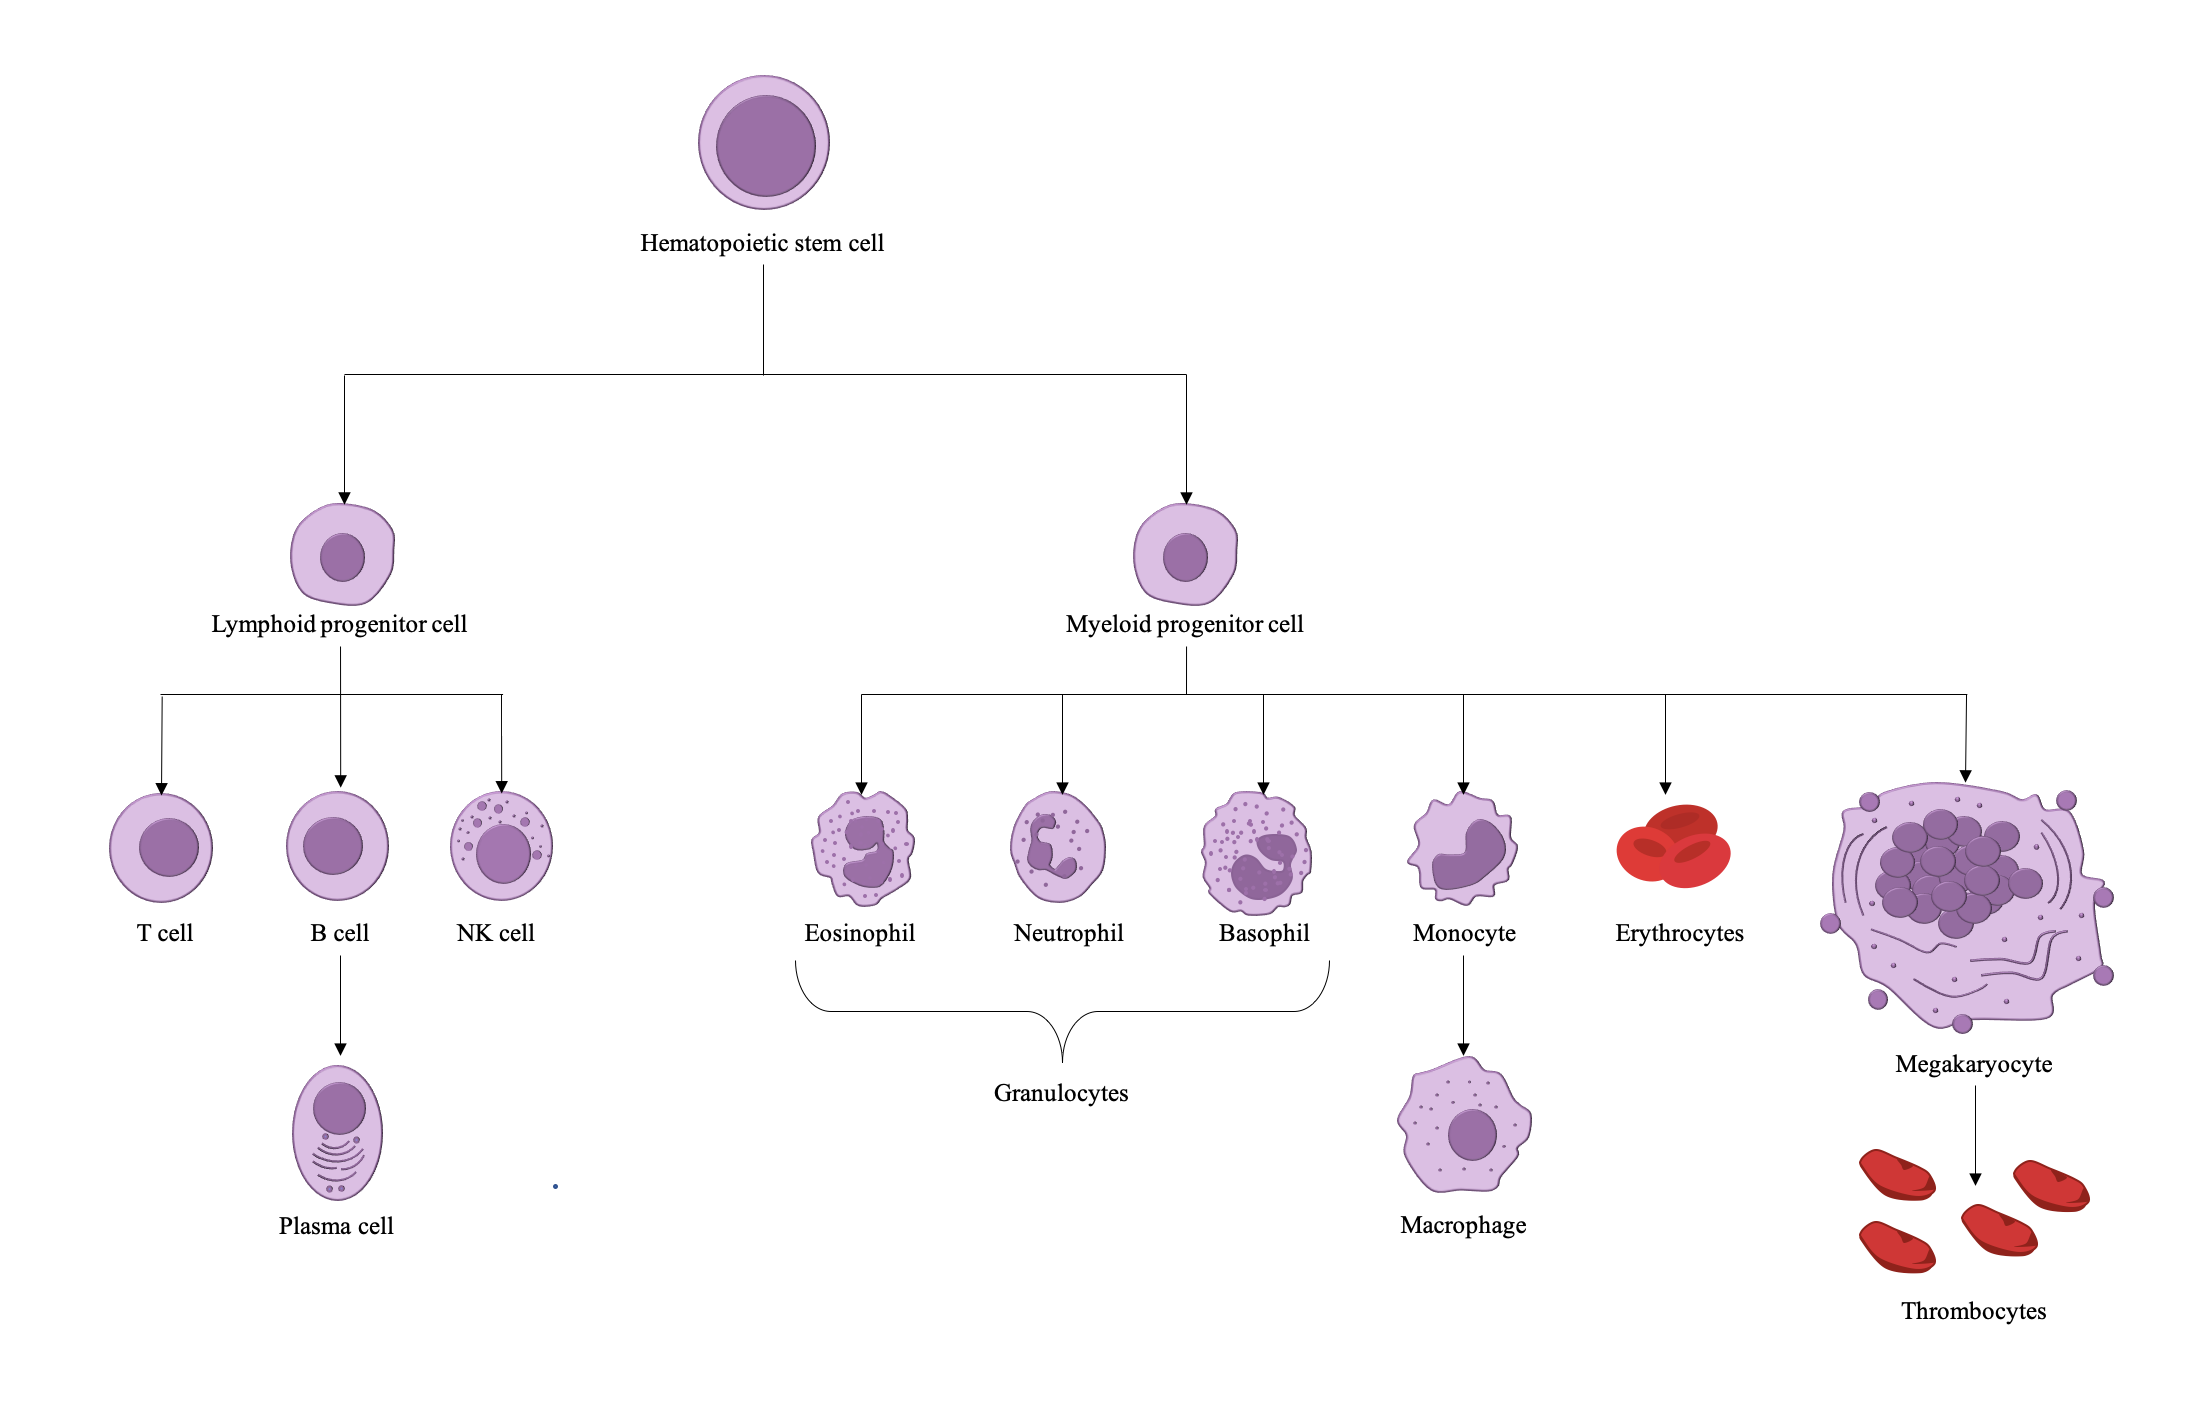
\includegraphics[width=0.7\textwidth]{figures/Introduction/immune_cells.png}
\caption[Hematopoietic system cell differentiation]{Hematopoietic stem cell (HSC) cell differentiation. HSCs divide into myeloid or lymphoid progenitor cells. Dendritic cells and a number of precursor states have been ommitted. }
\label{fig:HSC_differentiation}\end{figure}
%%

Most B cells die in the bone marrow soon after developing, however some will develop in the bone marrow, where initial stages of maturation occur and then migrate to secondary lymphoid organs, such as the spleen.
Within secondary lymphoid organs, numerous critical decisions on B cell fate are made, involving complex transcriptional networks, cell interactions, gene rearrangements, and mutations\cite{roth2014tracking, jourdan2011characterization}.
Upon antigenic-stimulation, naive B cells differentiate into memory B cells or plasma cells.
Terminally differentiated plasma cells are the final effectors of the B cell lineage, each dedicated to secreting large amounts of a single type of antibody.
Plasma cells have an extensive rough endoplasmic reticulum (ER), and have numerous genes involved in immunoglobulin secretion upregulated, including \textit{XBP-1} and \textit{CHOP}\cite{shapiro2004plasma}, to enable the production of copious amounts of antibody.
Plasma cells appear to consist of two distinct categories: short-lived plasma cells, which have life-spans of several months and are located in extrafollicular locales such as in medullary chords of lymph nodes or the red pulp of the spleen, and long-lived plasma cells, which have life-spans of decades and are mainly found in the bone marrow\cite{bortnick2013and, andraud2012living}.



%1
\section{Multiple myeloma}\label{sec:MM}
%2
\subsection{Multiple myeloma cells}
Multiple myeloma is a malignancy of terminally differentiated plasma cells.
It is characterised by aberrant proliferation of clonal, long-lived plasma cells in the bone marrow\cite{anderson2011pathogenesis}.
The large accumulation of MM cells in the bone marrow, crowd out healthy cells.
Under normal conditions, plasma cells produce antibodies that fight infection as part of the adaptive immune system.
However malignant plasma cells (MM cells) produce large amounts of abnormal antibodies that are unable to fight infection, coined `paraproteins' or `M proteins' (Figure \ref{fig:m_spike}).

%% M spike
\begin{figure}
\centering
\includegraphics[width=\textwidth]{figures/Introduction/M_spike.pdf}
\caption[M spike diagram]{Diagram of serum protein electrophoresis (SPEP) for a normal individual and for a multiple myeloma (MM) patient.
Based on their electrical charge, SPEP separates all the proteins in the blood.
A large peak is recorded for albumin (the most abundant protein in the blood), followed by lower levels of the other proteins, grouped into areas labelled $\alpha1$ and $\alpha2$, then a $\beta$ region, and then a $\gamma$ region, which represents where antibodies lie on the graph.
The large quantities of a single type of antibody (M protein) produced by MM cells cause a distinct `M spike' in the antibody protein region of the graph ($\gamma$ region).}
\label{fig:m_spike}
\end{figure}
%%

%2
\subsection{Epidemiology}
Multiple myeloma accounts for 1-2\% of all cancers and has the second highest incidence of hematological malignancies, after non-Hodgkin's lymphoma\cite{international2003criteria}.
MM is rare in individuals under the age of 40, with the average age at time of diagnosis centering around 70\cite{tsang2019multiple, palumbo2011multiple}.
MM is more prevalent in males than females and is around twice as common in black populations than in Caucasian or Asian populations\cite{nhsmyeloma}.
The average incidence rate is approximately 1-6 cases per 100,000 individuals\cite{tsang2019multiple, palumbo2011multiple, teras20162016}, with the highest age-standardised incidence rates in the regions of Australasia, North America, and Western Europe\cite{cowan2018global}.
Five-year survival rate of MM patients is approximately 49\%, whilst approximately a third of MM patients survive ten years or greater\cite{cancerresearchuk, siegel2016cancer}.
%While there have been many successful medicines developed for myeloma, they all suffer from the development of drug resistance.

%2
\subsection{Presentation}
%3
\subsubsection{Precursor states}
All cases of MM are preceded by asymptomatic precursor states, monoclonal gammopathy of unknown significance (MGUS) and smoldering multiple myeloma (SMM).
However, only some patients with SMM or MGUS progress to active MM.

MGUS is a pre-malignant condition where patients have the presence of monoclonal immunoglobulins in their blood or urine, $<$10\% clonal plasma cells in their bone marrow, but lack any myeloma-related end-organ damage\cite{van2018mgus}.
Patients with SMM have between 10 and 60\% clonal plasma cells in their bone marrow, serum monoclonal immunoglobulin of $\ge$3 g/dL, and like MGUS, have no signs of end-organ damage\cite{rajkumar2015smoldering}.
Progression risk of MGUS into symptomatic MM is about 1\% per year, whilst progression risk of SMM to MM is higher, at around 10\% per year for the first 5 years, after which it decreases\cite{korde2011monoclonal, kyle2007clinical}.
%

%3
\subsubsection{Active MM}
There are multiple classifications of active MM.
The International Myeloma Working Group's definition\cite{rajkumar2014international} is as follows:
Greater than 10\% clonal plasma cells located in the bone marrow and one or more myeloma-defining event or biomarker of malignancy.
Myeloma defining events consist of evidence of end-organ damage that can be attributed to the surplus of M protein and clonal plasma cells, namely the CRAB features:
%
% List of myeloma events (CRAB)
\begin{itemize}
  \item Hypercalcemia
    \begin{itemize}
        \item Serum calcium $>$ 1 mg/dL higher than the upper limit of normal, or
        \item Serum calcium $>$ 11 mg/dL
    \end{itemize}
  \item Renal insufficiency
    \begin{itemize}
        \item Creatinine clearance $<$ 40 mL per min, or
        \item Serum creatine $>$ 2 mg/dL
  \end{itemize}
  \item Anemia
    \begin{itemize}
        \item Hemoglobin value of $>$  20 g/L below the lower limit of normal, or
        \item Hemoglobin value $<$ 100 g/L
    \end{itemize}
    \item Bone lesions
      \begin{itemize}
        \item One or more osteolytic lesions on skeletal radiography, CT or PET-CT
        \end{itemize}
\end{itemize}
% End of list
%

Biomarkers of malignancy include greater than or equal to 60\% clonal plasma cells in the bone marrow, an involved:uninvolved serum free light chain ratio greater than or equal to 100, and more than one focal lesion on an MRI study\cite{rajkumar2014international}.

%
It is currently unclear what causes the malignant transformation between precursor states and active MM\@.
However certain factors have been identified as risk factors, including point mutations, a large array of up-regulated transcription factors, and numerous immune events.

\subsection{Treatment of multiple myeloma}\label{subsec:mm_treatment}
Multiple myeloma may be an incurable disease, however it is treatable.
In fact, in the last decade median survival time for newly diagnosed MM patients has almost doubled\cite{kazandjian2016look}.
Novel therapeutic advances have contributed to this improvement (Table \ref{tab:treatment_history}).
Myeloma is usually treated with a combination of drugs, often comprising a corticosteriod, a proteasome inhibitor, and an immunomodulatory drug (IMiD).
A common regimen, approved in the USA, European Union and UK for untreated myeloma is the triplet VRd regimen.
This consists of the proteasome inhibitor bortezomib (brand name Velcade), the IMiD lenalidomide (brand name Revlimid), and the corticosteroid dexamethasone.

% Timeline of treatment options
%% Table for treatment timeline


\begin{table}[h]
\centering
\begin{tabular}{|p{1cm}|p{3cm}|p{8cm}|p{1.3cm}|}
\hline
\textbf{Year} & \textbf{Treatment} & \textbf{Usage} & \textbf{Ref} \\ \hline
1958 & Melphalan & The alkylating agent melphalan was first used in plasma cell myeloma in 1958. & \cite{blokhin1958clinical} \\ \hline
1960s & Corticosteroids & Placebo-controlled double-blind trial of prednisone in multiple myeloma. Combinations of prednisone and melphalan showed an increased survival over melphalan alone. Dexamethasone and prednisone have become a cornerstone in the treatment of multiple myeloma. & \cite{mass1962comparison, alexanian1969treatment} \\ \hline
1980s & Stem-cell transplantations & Numerous successful allogenic and autologous bone marrow transplantations in patients with multiple myeloma &  \cite{mcelwain1983high, osserman1982identical, fefer1986identical, gahrton1987bone}  \\ \hline
2003 & Proteasome inhibitors & Bortezomib, a first-in-class proteasome inhibitor, was first approved by the FDA for use in relapsed and refractory multiple myeloma. In 2008 it was approved for patients with no prior treatment. Carfilzomib was approved in 2012 for advanced MM and later in 2015 for treatment of relapsed MM. The oral proteasome inhibitor, ixazomib, was approved as a combination treatment with lenalidomide and dexamethasone in 2016 for people who have received at least one previous treatment. & \cite{kane2003velcade,richardson2003phase,katsnelson2012next} \\ \hline
2006 & IMiDs & The antitumour activity of thalidomide was demonstrated in 1999, this led to the development of lenalidomide, the first approved immunomodulatory imide drug (IMiD) for use in multiple myeloma. Currently, thalidomide, lenalidomide and pomalidomide are approved for use in multiple myeloma & \cite{singhal1999antitumor,label47revlimid,san2013pomalidomide} \\ \hline
2015 & Monoclonal antibodies & In 2015, daratumumab, an anti-CD38 monoclonal antibody and elotuzumab, an anti-SLAMF7 monoclonal antibody, were approved for MM treatment. & \cite{lokhorst2015targeting,lonial2015elotuzumab} \\ \hline
\end{tabular}
\caption[Timeline of treatment options for multiple myeloma]{Timeline of treatment options for multiple myeloma. Listed by first usage or FDA approval for MM.}
\label{tab:treatment_history}
\end{table}

% https://www.ncbi.nlm.nih.gov/pmc/articles/PMC5282737/
% https://www.ncbi.nlm.nih.gov/pmc/articles/PMC2265446/
% Panobinostat	HDACi
% Liposomal doxorubicin	DNA inter-calator



\subsection{Proteasome inhibitors}
Proteasome inhibitors have contributed greatly to the improved prognosis of MM since their introduction into treatment regimes.
The first-in-class proteasome inhibitor bortezomib (Velcade\textsuperscript{\textregistered}) was approved by the FDA in 2003 as a single-agent for injection of relapsed MM\cite{kane2003velcade}.
Since then it has been approved for use in combination therapies.
Bortezomib in combination with melphalan-prednisone proved to be superior to the previous standard of care for patients ineligible for HDT-ASCT of melphalan-prednisone alone, increasing time until tumour progression\cite{san2008bortezomib}.
The combination of bortezomib, dexamethasone and thalidomide  was also shown to be superior to previous standard of care for patients prior to ASCT\cite{moreau2012proteasome}.
In 2010, bortezomib was approved as a frontline therapy for treatment-naive MM patients.
Since then, two more proteasome inhibitors have been approved, carfilzomib and ixazomib.
Carfilzomib is structurally and mechanistically different to bortezomib and shows activity on bortezomib resistant primary MM cells\cite{moreau2012proteasome}; it is approved for relapsed or refractory MM\@.

\subsubsection{The ubiquitin-proteasome system}
Proteasome inhibitors work by blocking the action of the proteasome in the cell.
Misfolded proteins can be harmful to a cell, so the combined activity of molecular chaperones, which aid in protein folding, and the ubiquitin-proteasome system (UPS), which acts to digest misfolded proteins, is needed to prevent massive protein aggregation.
Unneeded, misfolded or damaged proteins are tagged with lysine-48-linked poly-ubiquitin chains, marking them for degradation by the proteasome (Figure \ref{fig:26s_proteasome_structure}).
The proteasome is sometimes described as a complex `protein destruction machine'.
The proteasome consists of the 20S core particle, a central hollow cylinder, and the 19S regulatory caps associated with each end of the cylinder.
The 19S regulatory caps perform substrate recognition, deubiquitination, unfolding and threading of the protein substrate into the 20S core.
The core is made up of four stacked heptameric ring structures.
The outer rings are responsible for docking to the 19S cap and for acting as a gate to the inner rings. The inner rings consist of seven $\beta$ subunits, containing inward-facing protease active sites for degrading proteins\cite{kleiger2014perilous, alberts2007molecular} (Figures \ref{fig:26s_proteasome_structure} and  \ref{fig:proteasome_beta_subunits}).

 % Proteasome structure diagram
\begin{figure}[ht]
%1
\begin{subfigure}[t]{0.5\textwidth}
    \includegraphics[width=\textwidth]{figures/Introduction/26s_proteasome_serif.jpg}
    \caption{26S proteasome}
    \label{fig:26s_proteasome_structure}
\end{subfigure}
%\medskip
\begin{subfigure}[t]{0.5\textwidth}
    \includegraphics[width=\textwidth]{figures/Introduction/20s_core_beta_subunits_serif.jpg}
    \caption{$\beta$-subunits of an inner ring of the 20S core particle }
    \label{fig:proteasome_beta_subunits}
\end{subfigure}
    \caption[Structure of the proteasome]{Structure of the proteasome. \ref{fig:26s_proteasome_structure} shows the structure of the 26S proteasome, comprised of the 19S regulatory caps and 20S core particle.
    A misfolded protein tagged with a poly-ubiquitin chain is recognised by the 19s regulatory cap, which cleaves the ubiquitins from the protein and threads the protein through to the core, where it is degraded into small peptides.
    The 20S core particle is made up of two outer rings of $\alpha$-subunits and two inner rings of $\beta$-subunits.
    \ref{fig:proteasome_beta_subunits} shows the $\beta$-subunit arrangement in one of the inner rings of the 20s particle.
    $\beta1$ (caspase-like), $\beta2$ (trypsin-like) and $\beta5$ (chymotrypsin-like) are the proteolytically active subunits.
    Proteasome inhibitors are designed to primarily inhibit $\beta5$.}
\label{fig:proteasome_and_beta}
\end{figure}

\subsubsection{Mechanism of action}
Of the seven proteasome $\beta$ subunits, only $\beta1$, $\beta3$ and $\beta5$ are proteolytically active (Figure \ref{fig:proteasome_beta_subunits}). Proteasome inhibitors are designed to target $\beta5$ as it has been shown as the rate limiting protease for proteasomal protein turnover \cite{besse2019proteasome}. Bortezomib reversibly co-inhibits $\beta5$ and $\beta1$ subunits, whilst carfilzomib irreversibly binds to $\beta5$, with greater selectivity than bortezomib, and at higher doses binds to $\beta2$ as well \cite{besse2019proteasome}.


The precise downstream effects of $\beta$ subunit proteasome inhibition are not fully understood, however the unfolded protein response (UPR), NF-$\kappa$B signalling, JNK signalling, apoptotic factors and p53 are thought to be involved in the anti-MM effects \cite{kubiczkova2014proteasome}.
Specifically, the action of the UPR has been demonstrated as an important mechanism in the anti-MM effect of PIs.
MM cells secrete large amounts of monoclonal protein, leading to the rapid accumulation of  misfolded proteins within the endoplasmic-reticulum (ER) lumen.
This results in heightened ER stress, which is compensated by the UPR by reducing global protein translation and up-regulating UPS machinery \cite{wallington2018resistance}.
Therefore, by inhibiting the proteasome, fewer ubiquitin tagged proteins are degraded and more misfolded proteins accumulate in the ER lumen.
ER stress is then further increased, causing the UPR to switch from a homeostatic, pro-survival system to a pro-apoptotic pathway \cite{kubiczkova2014proteasome, wallington2018resistance}.

Another important mechanism for PI is the attenuation of NF-$\kappa$B signalling. I$\kappa$B$\alpha$, a specific endogenous inhibitor of the transcription factor NF$\kappa$B, is a protein degraded by the proteasome.
Inhibition of the proteasome increases levels of I$\kappa$B$\alpha$, thereby abolishing NF$\kappa$B signalling.
NF$\kappa$B is a key transcription factor in many cancers, contributing to overall tumour growth and chemoresistance.
NF$\kappa$B has been shown to promote tumour cell proliferation, anti-apoptotic and angiogenic factors \cite{kale2012molecular}.

\section{Drug resistance in multiple myeloma}
Although PIs are extremely effective at killing MM cells initially, long-term treatment inevitably results in a drug-resistant relapse.
Drug resistance is one of the biggest barriers in the treatment of MM.
Patients follow a pattern of peaks and troughs of treatment cycles, remission and relapse, until all therapies have little effect (Figure \ref{fig:treatment_cycles}).
%% Treatment cycles
\begin{figure}[htb]
\centering
\includegraphics[width=\textwidth]{figures/Introduction/treatment_cycles.pdf}
\caption[MM treatment cycles]{MM treatment cycles and disease progression over time.
All MM patients begin with precursor states Monoclonal Gammopathy of Unknown Significance (MGUS) and/or smoldering multiple myeloma (SMM) prior to a malignant transformation to symptomatic/active MM.
Patients undergo cycles of treatment, remission and relapse until eventually becoming relapsed and refractory (RRMM) and no longer respond to treatment.
}
\label{fig:treatment_cycles}
\end{figure}
%%
In order to overcome resistance and increase overall survival of MM patients, the molecular mechanisms of resistance to proteasome inhibitors needs to be understood.
This  will aid in the design of novel therapies and inform better use of existing therapies.
Previous studies on proteasome drug resistance have been performed and certain mechanisms and genes have been identified.
For example, point mutations have been noted in the \textit{PSMB5} gene (coding for the $\beta5$ subunit of the proteasome), as well as and over-expression of the $\beta5$ subunit \cite{robak2018drug}.
Other upregulated genes have been identified, for example \textit{ABCB1}, coding for P-glycoprotein, responsible for pumping various substrates out of the cell, also referred to as multidrug resistant protein 1.
\textit{XBP1}, involved in the UPR, has been seen to be downregulated in PI resistance \cite{robak2018drug}.
Although many genes have been identified to be differentially expressed in drug resistant MM, the mechanism is not fully elucidated and further research is imperative in the progression of treatment for multiple myeloma.

Another avenue to increase MM survival, would be to identify novel therapeutics effective against MM, which are capable of overcoming acquired anti-cancer drug resistance.
By increasing the arsenal of drugs available to treat MM, the time until patients become refractory and no longer respond to treatment could be prolonged.
Therapeutics with a novel mechanism of action are likely to be more effective for MM patients who have undergone several treatment cycles than drugs belonging to the same class as drugs they have previously been treated with.
Novel therapeutics would have less overlap of mechanism of action with existing drugs, therefore there would be less cross-resistance.

%
\afterpage{\clearpage} % flush out floats before this. Very different section
%
\section{Transcriptomics, proteomics and epigenomics}
It has been shown that changes in the genome, transcriptome, epigenome and proteome all contribute to disease progression and drug resistance in MM.
Therefore, to sufficiently investigate the multiple layers driving MM and to assess the effectiveness of new therapeutics, a multi-omics approach must be employed.

\subsection{DNA and the genome}\label{subsec:dna}
The genome is the genetic material of an organism, it consists of deoxyribonucleic acid (DNA).
DNA consists of two polynucleotide chains (or strands), running anti-parallel to each other, held together in a double helix structure by hydrogen bonds.
Nucleotides are composed of a five-carbon sugar (deoxyribose for DNA), attached to one or more phosphate group (a single phosphate group in the case of DNA) and a nitrogenous base.
Nucleotides are covalently linked to form an alternating sugar-phosphate backbone, with bases extending from each sugar towards the inside of the double helix.
Nucleotides contain four different types of bases: adenine (A), cytosine (C), guanine (G) and thymine (T).
The two DNA chains are held together by hydrogen bonds via complementary base pairing between the bases of the strands, A pairing with T and G pairing with C\@.
Often sections of DNA are denoted as their sequence of A, C, T and Gs (in order reading from the 5' to 3' direction).

Every individual has approximately 6 billion base pairs of DNA per cell, which would amount to about 2 metres of DNA if laid end-to-end.
The nucleus of a human cell is approximately 6\si{\micro\meter} in diameter, therefore chromosomal DNA must be folded tightly to fit.
DNA packaging is a complex task involving numerous speciliased proteins.
Negatively charged DNA is complexed with an octomer of positively charged proteins called histones to form nucleosomes.
The histone core is made up of eight subunits, two copies of H2A, H2B, H3 and H4 subunits.
DNA wraps tightly around the histone core 1.65 times.
Linker DNA connects adjacent nucleosomes, to resemble `beads on a string'.
Nucleosomes fold tightly to form 30\si{\nm} chromatin fibre, which in turns forms loops averaging 300\si{\nm} in length.
This fibre is folded and compressed again to form fiber 250\si{\nm} in width with loops of 700\si{\nm} in length.
Tight coiling of this fiber forms the single chromatids of chromosomes \cite{annunziato2008dna, alberts2002chromosomal}.
Human cells contain 23 pairs of chromosomes.

% DNA structure and packaging
\begin{figure}[htb]
%1
\begin{subfigure}[t]{0.5\textwidth}
    \includegraphics[width=\textwidth]{figures/Introduction/nucleotides_dna_helix.png}
    \caption{Nucleotide and DNA double helix structure}
    \label{fig:base_pairs}
\end{subfigure}
%\medskip
\begin{subfigure}[t]{0.5\textwidth}
    \includegraphics[width=\textwidth]{figures/Introduction/dna_packaging.png}
    \caption{DNA packaging}
    \label{fig:DNA_packaging}
\end{subfigure}
    \caption[DNA stucture and packaging.]{\ref{fig:base_pairs} shows the DNA nucleotides and the DNA double helix structure.
    DNA consists of two polynucleotide chains.
    Nucleotides are covalently linked to one another, forming a sugar-phosphate backbone.
    They contain one of four bases adenine (A), cytosine (C), guanine (G) and thymine (T).
    DNA strands are held together by hydrogen bonds between complementary base pairs, A pairing with T and G pairing with C\@.
    Sections of DNA are are often read by their sequence of bases from the 5' direction to the 3' direction.
    \ref{fig:DNA_packaging} shows how chromosomal DNA is packaged in the cell.
    DNA wraps 1.65 times around an octomer of histone proteins, to form a stucture called a nucleosome.
    Nucleosomes are linked by linker DNA to form a structure that resembles `beads on a string'.
    Nucleosomes fold to create chromatin fiber.
    This is turn forms loops and coils tighter and tighter until it makes up the single chromatids of chromosomes.
    \\\hspace{\textwidth}Created with BioRender.com.
    }
\label{fig:DNA_structure_packaging}
\end{figure}

The complete genome is made up of coding DNA (genes), non-coding DNA, as well as mitochondrial DNA and ribosomal DNA\@.
An alteration in the nucleotide sequence of the genome is called a mutation.
There are a number of types of mutations, including insertions, deletions, inversions, substitutions and duplications.
A technique called whole genome sequencing (WGS) can be used to determine the sequence of nucleotides in an individual's DNA and therefore it can be used to determine any variations in the genome.
% However the technique is expensive and many experiments are interested in coding DNA only, so perform RNA-seq to look at the transcriptome instead.

% Diagram double helix with bases in the middle. Then one of sequence of ACTG etc.
% Diagram of DNA genes transcribed to RNA then translated to proteins (pg 301 of textbook is good example)

\subsection{The epigenome}
Epigenetics is the study of any heritable phenotypic changes that do not involve alterations of the DNA sequence itself.
These changes occur at the chromatin level.
Epigenetic changes include histone modifications, DNA methylation and chromatin remodelling.
%These epigenetic changes are described in more detail below.

DNA methylation is the addition of methyl groups to the C5 position of cytosines in DNA.
This happens extensively at CpG sites (cytosine followed by a guanine).
Stretches of DNA with a high CpG ratio (CpG islands) are often found in the promoter region of genes.
Increased DNA methylation at CpG islands results in transcriptional silencing of those genes.
Genome wide DNA methylation is often examined using DNA-methylation-seq or DNA methylation microarrays.

DNA wraps tightly around histones (section \ref{subsec:dna}), they contribute to the tight packaging of DNA.
Histone modifications are post-translational modifications.
They include methylation, acetylation, phosphorylation, ubiquitination and sumoylation.
Histone modifications affect transcriptional activity either by directly influencing the structure of chromatin and DNA accessibility or by regulating binding of effector molecules to `read' histone marks to mediate downstream biological effects.
Histone modifications also regulate DNA processes, such as repair, replication and recombination \cite{ bannister2011regulation}.
Chip-seq can be used to investigate and measure various post-translational histone modifications.

Chromatin remodelling is the process of modifying chromatin architecture to regulate the accessibility of DNA.
Gene expression is regulated by allowing certain gene regions better access to transcription machinery.
This is achieved by ATP-dependent chromatin-remodelling complexes moving, ejecting or restructuring nucleosomes.
ATAC-seq can be used to identify accessible DNA regions.


\subsection{The transcriptome}
Transcription is the first of many steps in gene expression.
During transcription, the enzyme RNA polymerase reads a DNA sequence and produces an anti-parallel, complementary ribonucleic acid (RNA) strand.
The transcriptome is the set of all RNA transcripts of an individual.
RNA is a nucleic acid similar to DNA. Like DNA it has a sugar-phosphate backbone and 4 different types of bases attached to each sugar.
However, unlike DNA, RNA is single-stranded, it contains the sugar ribose in place of deoxyribose, and the nucleotide uracil (U) inplace of thymine (T).

Despite the chemical differences between DNA and RNA, they are essentially written in the `same language' and one-to-one mapping of nucleotides can be performed.
Transcription begins with the unwinding and opening of a small part of the DNA double helix, so bases are exposed.
One strand of DNA acts as a template and the RNA chain is formed by complementary base pairing with the template.
RNA polymerases catalyse the reaction of forming phosphodiester bonds between nucleotides, forming the RNA chain.
The RNA polymerase moves stepwise along the DNA chain, unwinding the chain just ahead exposing a new region of the template strand.
Just behind the region where ribonucleotides are being added, the DNA helix reforms.

The genes in a cell's DNA that specify the amino acid sequence and result in protein synthesis are called messenger RNA (mRNA) molecules.
Genes that produce the RNA molecule itself are called non-coding RNAs, because they do not code for proteins.
There are many other types of RNA, such as transfer RNA (tRNA), ribosomal RNA (rRNA) and micro RNA (miRNA).

Traditionally microarrays were used to measure gene expression.
Now RNA-seq (outlined in section  \ref{subsec:rna-seq-intro}) is more commonly used study to gene expression and the transcriptome.
Depending on the library preparation, different types of RNAs can be selected for or excluded, to study different RNA molecules.

\subsection{The proteome}\label{subsec:translation}
The proteome is the entire set of proteins that is or can be expressed by an organism.
mRNAs are translated into protein molecules.
mRNA is made up of only four different nucleotides, but proteins are made up of 20 amino acids, therefore a direct one-to-one function matching nucleotides to amino acids is impossible.
Instead, the sequence of mRNA is read in groups of three consecutive nucleotides, called a codon.
The three positions of a codon, and each position with four possible base options (A, C, U and G), gives a total of 64 different permutations (i.e. 4\textsuperscript{3}).
Therefore, some combinations map to the same amino acid (many-to-one function), or signal to terminate translation of the current protein, named a stop codon.
This genetic code directs the translation from mRNA to protein.
Translation takes place in the ribosome.

Codons on mRNA do not directly recognize their given amino acid, they require tRNA molecules that bind to both the codon on mRNA and the correct amino acid.
tRNAs possess an anticodon, a set of three nucleotides complementary to a given codon.
Firstly, tRNAs are coupled to their cognate amino acid.
This reaction is catalysed by aminoacyl-tRNA synthetase (aaRS) enzymes.
aaRSs attach amino acids to the 3' end of tRNA.
Most cells have a specific aaRS for each amino acid.
Once the tRNA is charged with the correct amino acid, the tRNA molecule binds to its complementary codon on mRNA.
Subsequent aminoacylated tRNA molecules bind to mRNA codons.
A polypeptide chain grows by stepwise addition of amino acid to the C-terminal end.
The formation of the new peptide bond between amino acids releases the tRNA molecule.
The peptide chain grows until a stop codon is reached and synthesis of the current protein is complete.

Protein translation is partly regulated by availability of mRNAs, but it also depends on other factors such as RNA silencing and post-transcriptional modifications.
Proteins have a large array of functions, such as transporting small molecules, catalysing reactions, cell-cell signalling and providing structural support.

Proteomics is the study of the proteome.
CyTOF and LC-MS/MS are techniques often employed to examine the proteome. %(section \ref{subsec:cytof-intro} and section \ref{subsec:lcmsms-intro}).

\subsection{Sequencing}
DNA is often referred to as the `genetic master code', therefore the ability to decode the order of nucelic acids has been seen as a highly desirable feat since its discovery.
Sequencing is the process of determining the sequence of nucleotides of nucleic acid residues.
Over the last half-century, large numbers of researchers and vast sums of money have been applied to facilitate the techniques and technologies to decode DNA and RNA molecules' nucleotide sequence \cite{heather2016sequence}.
Over this time, massive technological innovations have been developed.
The most commonly used `first-generation' DNA-sequencing technology, Sanger sequencing, was developed in 1977 \cite{sanger1977dna}.
In Sanger sequencing, or the `chain termination method', chain-termination PCR is performed with a mix of regular nucleotides (deoxynucleotide triphosphates; dNTPs) and fluorescently-labelled, chain-terminating dNTPs (dideoxynucleotide triphosphates; ddNTPs), using the DNA of interest as a template.
During the extension step of PCR, when DNA polymerase incorporates a ddNTP randomly, extension ceases.
This creates greater than a million copies of the DNA sequence of interest, all terminated at random lengths by the ddNTPs.
Capillary gel electrophoresis is then used to separate the extension products by size.
The gel is then read to determine the sequence.
By reading the gel bands from smallest to largest, the 5' to 3' sequence of the original DNA strand can be inferred.
Sanger sequencing was used by the Human Genome Project, an international research effort to determine the DNA sequence of the entire human genome \cite{pennisi2001human}.
The whole project took approximately 13 years to complete, and was reported to have cost \$3 billion.

Sanger sequencing dominated the sequencing world for over 30 years, until the advent of `Next-generation sequencing' (NGS; now being dubbed `second-generation sequencing', with the advent of newer technologies).
NGS differs from its predecessors in that it is highly scalable and massively parallel.
With NGS you can rapidly sequence the entire human genome in one day, for just under \$5000.
It is quicker and cheaper than traditional Sanger sequencing, and has progressed data output from the kilobase range up to potentially multiple terabases per run.
Today, the largest and most commonly used NGS sequencing technology platform is Illumina, who own around 80\% of the global sequencing market.
NGS can be used to study the transcriptome, using RNA-seq techniques (Section \ref{subsec:rna-seq-intro}); the epigenome, using techniques such as ChIP-seq or ATAC-seq; or the genome using techniques such as whole genome sequencing (WGS).

Recently, long-read technologies are becoming more prominent in the sequencing field.
Illumina short-read sequencing limits read length to between 50 and 300 base pairs (bp)\@.
This read length is too short to detect more than 70\% of human genome structural variation.
Moreover, some of the most mutation-prone regions of the genome are inaccessible due to repeating or GC-heavy content, limiting sequence coverage and leaving large regions of the genome critically understudied \cite{logsdon2020long}.
Long-read technologies are capable of generating continuous sequences ranging from 10 kilobases to several megabases, enabling the sequencing of full-length transcripts.
The two main emerging long-read technologies are PacBio single-molecule real-time (SMRT) sequencing\cite{wenger2019accurate} and Oxford Nanopore Technologies (ONT) sequencing\cite{ip2015minion, jain2016oxford}, together marking the birth of `third-generation sequencing' (TGS).
Both PacBio and ONT sequencing sequence single DNA molecules, rather than a pool of PCR-amplified fragments.
PacBio sequencing employs a sequencing-by-synthesis strategy (similar to Illumina sequencing), with circular DNA templates to improve accuracy.
ONT sequences a native linear single-stranded DNA molecule by measuring current changes as bases are threaded through a nanopore \cite{weirather2017comprehensive}.
Whilst TGS technologies have the advantage of longer read length, the methods are also plagued by higher base-calling error rates and lower throughput than NGS technologies \cite{weirather2017comprehensive, philpott2021nanopore}.
Therefore, this makes applying TGS to single-cell RNA-seq especially challenging.
Due to the lower through-put, fewer cells can be reported on at a comparable read-depth to NGS technologies;
and due to the high base-calling error rate, inaccurate cellular and molecular barcode assignment can complicate associating mRNA reads with their cell of origin.

\subsection{RNA-seq}\label{subsec:rna-seq-intro}
Most modern RNA sequencing (RNA-seq) implements NGS technology to analyse RNA across the transcriptome of a biological sample and allows for the quantification of gene expression.

\subsubsection{Bulk RNA-seq}
Bulk RNA-seq measures the average expression across a sample.
Creating a bulk RNA-seq library involves isolating RNA from a biological sample, filtering for a specific type of RNA (most commonly mRNA), fragmentation of RNA into fragments, reverse transcription of the fragments to generate a complementary DNA (cDNA) library, end repair and adaptor ligation of the cDNA library, followed by PCR amplification ready for sequencing.

%% Diagram of bulk RNA-seq
\begin{figure}[ht]
\centering
\includegraphics[width=0.8\textwidth]{figures/Introduction/bulk_rna_library_prep_diagram_alternate.png}
\caption[Bulk RNA-seq outline]{Outline of bulk RNA-sequencing library prep.
Cells are lysed and RNA is extracted.
The specific RNA of interest is selected and enriched, for example selecting for mRNA using polyA selection or ribo-depletion.
The mRNA is fragmented into smaller pieces of RNA.
First and second stranded cDNA are reverse transcribed from the RNA fragments using random primers.
The ends of the cDNA are repaired and dAMP (dA) tails are added to the 3' end of the DNA.
Adaptors are ligated to the 3' and 5' end of the cDNA.
These adaptors contain complementary sequences that allow the fragments to hybridize to the flow cell during sequencing.
Universal (P5/i5) and index (P7/i7) primers are added to the adaptor ligated DNA.
The libraries are then amplified using PCR and cleaned-up, ready for sequencing.
}
\label{fig:bulk_diagram}\end{figure}
%%

\subsubsection{Single-cell RNA-seq}
Single-cell RNA-seq (scRNA-seq) measures gene expression for each individual cell across a population of cells and therefore provides information on clonal diversity that may be lost when pooling cells into bulk samples.
Since its inception in 2009\cite{tang2009mrna}, there have been numerous scRNA-seq techniques developed, such as SMART-seq2\cite{picelli2013smart}, Drop-seq\cite{macosko2015highly}, STRT\cite{islam2011characterization}, scCOLOR-seq\cite{philpott2021nanopore} and inDrops\cite{klein2015droplet}.
scRNA-seq library preparation shares many steps with bulk RNA-seq workflow, however preliminary steps are required to isolate single cells and barcode reads that originated from the cell.
%% Diagram of drop-seq
\begin{figure}[hb]
\centering
\includegraphics[width=0.7\textwidth]{figures/Introduction/drop_seq.png}
\caption[Drop-seq schematic]{Outline of Drop-seq, a droplet-based scRNA-seq method.
A microfluidic device combines two aqueous flows, one containing cells and the other containing barcoded primer beads suspended in lysis buffer.
The two aqueous channels flow across an oil channel to form aqueous droplets surrounded by oil.
Relatively few droplets contain both a cell and a bead.
Following droplet formation, the cell is lysed and its mRNAs are released, which then hybridise to the primers on the bead surface.
A reagent is added to break up the droplets and the beads are collected and washed.
The mRNAs are reverse-transcribed into cDNAs, generating a set of ``STAMPS'' (single-cell transcriptomes attached to microparticles) and template switching is used to introduce a PCR handle.
The barcoded STAMPS can then be amplified using PCR.}
\label{fig:dropseq}\end{figure}
%%
For droplet-based scRNA-seq (dscRNA-seq) methods, single cells are isolated using microfluidic devices by individually encapsulating them in aqueous droplets contained in oil.
Below, a dscRNA-seq method, Drop-seq, is outlined (Figure \ref{fig:dropseq}).


% \subsection{ATAC-seq}

%\subsection{ChIP-Seq}
%Chromatin immunoprecipitation sequencing (ChIP-seq) is used to analyse protein interactions with DNA.
%At a base-pair resolution, it is used to map DNA-binding proteins and histone modifications.
%Therefore ChIP-seq is often used to determine the the mechanisms of gene regulation of transcription factors, and to study epigenetic mechanisms in detail.
%It utilises NGS to identify biding sites of DNA-associated proteins, therefore it is often used to determine the mechanisms of transcription factors or chromatin-associated proteins, influencing gene expression.


%\subsection{CyTOF}\label{subsec:cytof-intro}


%\subsection{Liquid chromatography with tandem mass spectrometry}\label{subsec:lcmsms-intro}
%Liquid chromatography with tandem mass spectrometry (LC-MS/MS) based proteomics is a popular analytical technique to measure the protein abundance of a sample.
%The general steps for LC-MS/MS-based proteomics include: cell lysis, protein extraction, protein digestion using an enzyme to cleave proteins into peptides, peptide purification, and analysis by mass spectrometry.
%The resultant data includes mass and charge (m/z) information and peak intensities.
%Software is then employed which performs database searches and calculates the most likely peptide for each peak.
%From this data, protein abundance can then be calculated and normalised.

%LC-MS/MS-based proteomics can also be used to search for specific proteins within the proteome.
%For example, immobilized metal affinity chromatography (IMAC) can be used to enrich for phosphorylated peptides (phosphoproteomics), and anti-ubiquitin antibodies can be used to enrich for ubiquitinated peptides (ubiquitinomics).

%\section{Summary}

\section{Thesis aims and chapter outline}
This thesis aims to identify novel therapeutics with anti-MM properties, capable of overcoming acquired drug resistance in MM\@.

\noindent
Chapter \ref{ch:1-intro}: General introduction of the adaptive immune system, multiple myeloma (MM) and treatment of MM, as well as an introduction into the multiple layers of information underpinning life: the genome, transcriptome, epigenome and proteome, and the different multi-omic techniques that can be employed to investigate them.

\noindent
Chapter \ref{ch:2-litreview}: Literature review introducing aminoacyl-tRNA synthetases (aaRS), the roles they play in disease and therapeutics targeting aaRSs, focusing on the prolyl-tRNA synthetase inhibitor, Halofuginone (HF) and its applications, particularly in multiple myeloma.

\noindent
Chapter \ref{ch:3-methods}: Experimental materials and methodology used in this work.

\noindent
Chapter \ref{ch:4-Pipelines}: Outline of computational methods generated to support experimental work and benchmark validations of their effectiveness.

\noindent
Chapter \ref{ch:5-bulk}: Investigation of the use of ProRS inhibitors in PI-sensitive and PI-resistant MM cell lines.
Bulk-RNA seq is employed and the transcriptional landscape following ProRS treatment is characterised.

\noindent
Chapter \ref{ch:6-sc}: Exploration of ProRS inhibitor treatment of primary BM samples from MM patients at the single cell level.
Their effectiveness against newly-diagnosed and relapsed MM patient tissue is investigated.

\chapter{\label{ch:2-litreview}Aminoacyl tRNA synthetases and Halofuginone}

\section{Introduction}
Aminoacyl tRNA synthetases (aaRS) are a highly-conserved family of enzymes, responsible for ``charging'' tRNAs with their cognate amino acid.
Human cytoplasmic aaRSs are either ``free'' as individual species or bound in a macromolecular complex, comprised of eight aaRSs and three auxiliary proteins, known as the multi-tRNA synthetase complex (MSC).
On top of their canonical enzymatic role, aaRSs also engage in non-enzymatic functions in numerous pathways, including angiogenesis, inflammation and metabolism.
Often species are released from the MSC to regulate these non-canonical activities.
aaRSs have been shown to involved in numerous diseases, including cancer.
Initially, due to their high fidelity and complex evolution over millennia, aaRSs were seen as an attractive drug target for antimicrobials, to enable specifically targeting microbial aaRSs with minimal effects on human cells.
The mechanism of action of Febrifugine (FF), a quinazoline alkaloid that has long been used as an antimalarial remedy, has recently been revealed; it acts as a competitive inhibitor of ProRS (part of the bifunctional glutamyl-prolyl-tRNA synthetase enzyme; EPRS), responsible for charging tRNA\textsuperscript{pro} with proline.
Although it has potent antimalarial effects, Febrifugine exhibits high liver and gastrointestinal (GI) toxicity, so cannot be used as a widespread drug, therefore several analogues of Febrifugine were developed in the hope of minimizing toxicity to the host`s cells.
One such analogue, Halofuginone (HF) was synthesized and was shown to have the most potent antimalarial properties of all the derivatives, with lower toxicity to the host than Febrifugine, but still some liver toxicity and GI side effects remain.
Halofuginone has been applied to and showed promise in many other non-parasitic diseases too.
It has received orphan drug status for scleroderma and HIV-Related Kaposi's Sarcoma.
Recently, Halofuginone`s application in various cancers has become of great interest, including but not limited to: metastatic brain tumours, bladder carcinomas, prostate cancer, renal carcinomas, hepatocellular carcinomas, lung cancer, breast cancer and multiple myeloma.


This review will introduce the structure and function of aminoacyl tRNA synthetases, provide an insight into their role in pathology and potential as therapeutic targets.
EPRS1 and its inhibitors will be the primary focus, and exploring...

\section{Function and structure of aminoacyl tRNA synthetases}

Aminoacyl tRNA synthetases (aaRS) are an ancient family of ubiquitous enzymes, conserved across three major domains of life (but not present in viruses).
They can be traced back prior to the ``Last Universal Common Ancestor'' (LUCA) \cite{de2020evolution}.
aaRSs are essential for protein biosynthesis, and catalyse the first step in translation (see section \ref{subsec:translation}).
aaRSs catalyse the charging of tRNAs with their cognate amino acid.
This is a two-step process.
Firstly, aaRSs catalyse the formation of an aminoacyl-adenylate (activated amino acid) from their corresponding amino acid and an ATP molecule, releasing an inorganic pyrophosphate.
Next, aaRSs catalyse the reaction between the aminoacyl-adenylate and their cognate tRNA to release an AMP molecule and generate an aminoacyl (charged)-tRNA, ready to be used by the ribosome to decode mRNA (see equation \ref{eqn:aminoacyl}).
An example of this process would be prolyl-tRNA synthetase (abbreviated to ProRS) charging tRNA\textsuperscript{pro} with proline.

\begin{equation}\label{eqn:aminoacyl}
\begin{gathered}
aa + ATP \rightleftharpoons  aa.AMP + PPi \\
aa.AMP + tRNA^{aa} \longrightarrow  aa.tRNA^{aa} + AMP
\end{gathered}
\end{equation}

Eukaryotes have 20 cytoplasmic aaRS and 20 nuclear-encoded mitochondrial aaRS.
These are localised in distinct cellular compartments.
aaRSs are often denoted by their one letter amino acid symbol, followed by ARS and either 1 (indicating they are cytoplasmic) or 2 (indicating they are mitochondrial), for example PARS1 for cytoplasmic ProRS.
This review will focus on cytoplasmic aaRS enzymes.
aaRS can be divided into two distinct classes based on the structure of the fold of their catalytic domains.
Class I aaRS enzymes are functional monomers that contain a dinucleotide or Rossman fold (RF) of alternating alpha-helices and parallel beta-sheets.
This fold is where ATP and amino-acid binding takes place and therefore facilitates the aminoacylation reaction.
The active site of class I aaRS is marked by the signature motifs ``HIGH'' (His-Ile-Gly-His) and ``KMSKS'' (Lys-Met-Ser-Lys-Ser).
Within the first half of the RF the HIGH motif helps to correctly position the adenine base of ATP and interacts with the phosphates.
The second K of the KMSKS motif is thought to be involved in stabilising the transition state for the primary step of aminoacylation \cite{newberry2002structural}.
Amino acid recognition and binding takes place in the catalytic site when the KMSKS motif is open.
The KMSKS loop closes after the aaRS binds ATP and the aminoacyl-adenylate is formed \cite{kwon2019aminoacyl}.


Class II aaRS enzymes are functional dimers or tetramers with an uncommon catalytic core, comprising seven anti-parallel beta-sheets, flanked by alpha-helices.
Class II aaRS enzymes are defined by three conserved sequence motifs.
Motif 1 is located at the interface of the dimer and enables oligomerization.
Motifs 2 and 3 comprise part of the aminoacylation active site and facilitate amino acid/ ATP binding and adenylate formation.
Motif 3 binds ATP, and motif 2 is involved in coupling ATP and the amino acid and then transferring the amino acid to the 3`-tRNA \cite{kwon2019aminoacyl}.
The distinct active-site structures of class I and II enzymes confer markedly different binding mechanisms for the aminoacylation reaction.
For example, class I aaRSs bind the tRNA acceptor stem via the minor groove side and bind ATP in an extended conformation, whilst class II aaRSs bind the tRNA acceptor stem from the major groove side and bind ATP in a bent conformation.
The two classes of aaRSs split the twenty amino acids into two groups.
Val, Leu, Ile, Met, Glu, Gln, Trp, Tyr, Arg and Cys are activated by their cognate class I aaRS; and Gly, Pro, Ala, Thr, Ser, Hist, Asp, Asm, Lys and Phe are activated by their cognate class II aaRS.
Class I and class II can be further divided into different sub-groups, however that is beyond the scope of this review.
The structural diversity of aaRSs is likely attributable to the need to exclude similar non-cognate amino acids and to discriminate the correct tRNA isoacceptor.

Both class I and class II aaRSs are multi-domain proteins- in addition to their catalytic domains, they include other domains such as their anti-codon recognition domain or an editing domain.
The editing domain found in some aaRSs is to ensure that the essential step of aminoacylation in protein biosynthesis is as accurate as possible, so incorrect amino acids can be removed from aminoacyl-adenylates or mischarged tRNAs \cite{kwon2019aminoacyl}.
Theoretically, it was estimated that mistranslation rate should be approximately 1 in 200 for amino acids differing by just a methyl group (such as valine and isoleucine) \cite{pauling1958festschrift}, however in-vivo work demonstrated that the error frequency is closer to 3 in 10,000 (approximately 1 in 3000) \cite{loftfield1972frequency}.
This suggested the existence of proof-reading capabilities of aaRSs, to account for the difference between observed and predicted error rates.
Editing capability has since been shown to be of high functional importance to some aaRSs.
For example, a study in mice in which there was a missense in the editing domain of AlaRS.
The impaired proof reading activity of the enzyme lead to an accumulation of misfolded proteins, resulting in the activation of the unfolded protein response and substantial neurodegeneration \cite{lee2006editing}.
Not all aaRSs possess editing activity, only about half do, however the high specificity of the active site of those aaRSs is enough to alleviate proofreading need.

\subsection{Multi-tRNA synthetase complexes}
Higher eukaryotes contain macromolecular complexes, which consist of nine enzymes and three auxiliary proteins, known as multi-tRNA synthetase complexes (MSC).
The 11 cytoplasmic aaRSs not located in the MSC remain free as individual species.
The nine cytoplasmic aaRS enzymes of the MSC are GluRS (EARS1), ProRS (PARS1), IsoRS (IARS1), MetRS (MARS1), GlnRS (QARS1), LysRS (KARS1), ArgRS (RARS1), AspRS (DARS1), LeuRS (LARS1).
GluRS and ProRS are covalently fused via triple repeats of WHEP domains to form a bifunctional enzyme, EPRS1.
The non-enzyme component of the MSC consists of three aminoacyl-tRNA synthetase-interacting multifunctional proteins (AIMP), AIMP1, AIMP2 and AIMP3.
Human MSCs contain more class II aaRS enzymes than other species, namely DARS1, KARS1, and PARS1, they also contain more auxiliary proteins.
Human MSC components have several additional domains or motifs (Figure \ref{fig:MSC}A), for instance GST-homology domains in EPRS, MetRS, AIMP1 and 2, and WHEP domains in EPRS and MetRS \cite{kim2019evolution, khan20203, kim2020structures}.

The structure of human MSC has not been fully elucidated, however some sub MSC-complex structures have been revealed.
LysRS forms a homodimer and is anchored to the N-terminal peptide region of AIMP2 within the main body of the MSC.
MetRS, AIMP3, EPRS1 and AIMP2 are compactly linked through their GST-homology domains.
ArgRS, GlnRS and AIMP1 assemble into a heterotrimeric complex \cite{kim2019evolution, khan20203, kim2020structures}.
A proposed bisymmetrical model of the human MSC, via homodimerization of AspRS and ProRS, is shown in Figure \ref{fig:MSC}B, based on subcomplex and interaction data \cite{cho2015assembly, kaminska2009dissection, mirande2017aminoacyl}.
This hypothesis proposes that the MSC is a super-complex of two identical, symmetrically arranged subunits (symmetrical along the y-axis in Figure \ref{fig:MSC}B), each containing one copy of the constituent elements, except for LysRS which is present as a dimer in each subunit.

%% Diagram of MSC
\begin{figure}[htb]
\centering
\includegraphics[width=0.6\textwidth]{figures/lit_review/MSC_structure.jpg}
\caption[Multi-tRNA synthetase structure]{The human multi-tRNA synthetase (MSC) and its components.
\textbf{A)} The domains of the aminoacyl tRNA synthetases and auxiliary proteins (AIMP1, 2 and 3) making up the human multi-tRNA synthetase (MSC).
The bifunctional enzyme EPRS1 is made up of the class 1 enzyme GluRS and class II enzyme ProRS (dimer) covalently linked by three WHEP domains.
\textbf{B)} Cartoon representation of a proposed bisymmetrical model structure of the human multi-tRNA synthetase complex (MSC).
An adaption of a figure created by Myung Hee Kim and Sunghoon Kim \cite{kim2020structures}.
}
\label{fig:MSC}\end{figure}

The function of the MSC was originally thought to be to increase efficiency of protein biosynthesis by localising aaRSs.
Another proposed function of the MSC was to increase stability of its components.
It has been shown using systematic depletion analysis that some of the components are in fact intrinsically less stable in isolation and dependent on their neighbours for stability \cite{han2006hierarchical}.
More recently, examples have emerged where the MSC seems to work as a `molecular reservoir' which can control the release of its components.
The release of components from the MSC has been linked to numerous non-canonical pathways, including cell signalling, metabolism, inflammation and angiogenesis.

Higher eukaryotes usually have extra-domains at the N- or C- terminus of aaRS enzymes compared with lower eukaryotes and prokaryotes, which may partly contribute to MSC assembly.
Most human cytoplasmic aaRS enzymes have at least one new sequence extension or domain, most of which are dispensable for enzymatic activity, suggesting they may contribute to the non-canonical roles of aaRS.
Additionally, aaRSs are often found in the nucleus of cells, where protein biosynthesis does not occur.
The additional evolutionary complexity in human aaRSs and MSC seems to explain the increased physiological complexity and their functionality in non-enzymatic processes.

Examples of non-canonical MSC functionality include--- LARS1 translocating from the MSC to lysosomes, facilitating mTORC1 activation \cite{han2012leucyl}; KARS1 translocating to the nucleus upon immune activation and activating MITF-dependent gene expression in mast cells \cite{yannay2009lysrs}.
Another example is EPRS1 release from the MSC in myeloid cells upon IFN-$\gamma$ stimulation \cite{arif2009two}.
IFN-$\gamma$ induces a network of kinase events (Cdk5, mTORC1 and S6K1 activation) which causes a two-step phosphorylation of two serines in the linker region of human EPRS, and causes its release from the MSC.
EPRS1 combines with other proteins (namely NSAP1, L13a and GAPDH) to form the cytosolic IFN-$\gamma$ activated inhibitor of translation (GAIT) complex, which represses translation of numerous inflammatory-related transcripts, including VEGFA and ceruloplasmin \cite{arif2018gait}.


In addition to the enzymatic components of the MSC, the auxiliary proteins AIMP1, 2 and 3 are also involved in fundamental biological processes.
AIMPs exhibit non-canonical functions aside from their roles as scaffolds in the MSC.
AIMPs have been linked to numerous biological processes, including involvement in immune regulation, nervous system functions, viral replication, genome stability, angiogenesis, and cancer.
AIMP1 interacts with RARS1 and facilitates incoming tRNA substrates to its catalytic site to enhance its enzymatic activity \cite{park1999precursor}.
In addition to improving amino-acyl synthetase activity, secreted AIMP1 has also been shown to be involved in angiogenesis, inflammation induction, wound closure, and maintaining glucose homeostasis \cite{park2006hormonal}.
TGF-$\beta$ and the DNA damage response have both been shown to cause phosphorylation of AIMP2 and disassociation from the MSC.
Released AIMP2 has shown to act as a pro-apoptotic mediator and tumorigenesis suppressor via various pathways \cite{zhou2020roles}.
AIMP3 largely interacts with MARS1, and under conditions initiating the DNA damage response, MARS1 undergoes a conformational change that releases AIMP3 from the MSC \cite{kwon2011dual}.
Released AIMP3 acts as a tumour suppressor, translocating to the nucleus and upregulating expression of the tumour suppressor gene p53.

The functional and structural complexity of the MSC is still being revealed.
The canonical and non-canonical functionality of MSC components promises an unexplored rich source of potential therapeutic targets, but also lends itself to associated pathology.

\section{aaRSs in disease}
With the diversity of functionality in human aaRSs comes an increase in functionality that can be associated pathologically with human disease.
Structural and functional variations in aaRSSs' enzymatic and non-enzymatic activities have been linked to various human diseases.
Changes in gene expression, copy number, mutations and genetic variations of aaRSs have been documented in relation to disease \cite{kwon2019aminoacyl}.

Charcot Marie Tooth (CMT) is a genetically and clinically-presenting heterogeneous group of hereditary peripheral neuropathies.
CMT is characterised by progressive degeneration of distal sensory and motor neuron function \cite{yao2013aminoacyl}.
Six aaRSs have been linked to CMT through dominant mono-allelic mutations, including GARS1 and YARS1, which are among numerous genetic-loci to have been linked causally to CMT.
Drosophila models of CMT have demonstrated that CMT-causing YARS1 mutations lead to a conformational change in YARS1, leading to aberrant interactions with transcriptional regulators in the cell nucleus and aberrant expression of certain transcription factors \cite{bervoets2019transcriptional}.

aaRSs have also been implicated in autoimmune diseases.
``Anti-synthetase syndrome'' (ASS) is a heterogeneous group of autoimmune diseases, including interstitial lung disease (ILD), arthritis, idiopathic inflammatory myopathies, myositis and Reynaud's phenomenon.
Autoimmune antibodies against histidyl-, threonyl-, alanyl-, isoleucyl-, phenylalanyl-, glycyl-, tyrosyl-, asparaginyl-tRNA synthetase have been found in approximately 30\% of all autoimmune patients.
Dysregulation of aaRS has also been noted in other autoimmune diseases, for example multiple sclerosis and immune thrombocytopenia \cite{nie2019roles}.

aaRSs have been linked to viral and bacterial infection.
For example, it has been shown that viral infection leads to the phosphorylation of EPRS and dissociation from the MSC, ultimately blocking PCBP2-mediated mitochondrial antiviral signalling (MAVS) ubiquitination and inhibiting viral replication \cite{lee2016infection}.
Additionally, HIV-1 infection leads to KRS release from the MSC, which is partially transported to the nucleus.
Blocking this release reduced the infectivity of progeny virions, implying that HIV-1 utilizes a dynamic MSC for enhanced viral replication \cite{duchon2017hiv}.
WARS1 was shown to be increased approximately 27-fold in sepsis patients with a bacterial infection compared with healthy controls. Following a range of infections by various pathogens, host monocytes were shown to rapidly secret WRS.
The secreted WRS increased cell surface levels of CD40, CD80 and CD86, markers of macrophage activation \cite{ahn2016secreted}.

\subsection{aaRSs in cancer}
A growing number of studies have implicated aaRSs and MSC components in tumorigenesis.
Firstly, aaRS enzymatic activity is essential to sustain tumour growth. In cancer metabolism, biosynthesis of aminoacyl-tRNAs has been shown to be highly up-regulated [hu2013heterogeneity].
In cancer, we see often see dramatic rapid cell growth, this demands an intense increase in overall protein synthesis. To keep up with this demand, the canonical aminoacylation role of aaRSs is crucial as the first step in protein synthesis.

On top of the enzymatic role of aaRSs, their non-canonical functionality has also been associated with both promoting and inhibiting cancer.
The hallmarks of cancer- enhanced growth signalling and proliferation, vascularization, metastasis, altered metabolism, and immune/tumour microenvironment invasion, all have links to tRNA synthetase function.
Cancer cells require enhanced growth signalling and proliferation to maintain their rapid growth beyond the capacity of normal cells, several aaRSs have been linked to this aberrant growth signalling.
GlyRS has been shown to be integral for cancer-promoting neddylation to occur, and reduced MetRS expression resulted in reduced tumorigenicity in p16INK4a-negative breast cancer cells in vivo \cite{mo2016neddylation, deng2020role, kwon2018stabilization}.
For tumours to grow and metastasize they need to hijack existing vasculature to get blood flow to growing area, or make new vessels by promoting angiogenesis.
Endothelial cells (EC) exposed to TNF-$\alpha$ or VEGF secrete ThrRS.
ThrRS promotes EC migration and angiogenesis.
Inhibition of ThrRS was shown to inhibit angiogenesis, with and without inducing the uncharged tRNA response \cite{williams2013secreted, mirando2015aminoacyl}.
LysRS has been shown to support metastasis by increasing migration.
Following phosphorylation by the MAPK pathway, LysRS binds to the 67kDa membrane bound laminin receptor protein (67LR), preventing its degradation and sustaining laminin-dependent migration.
Once bound to LysRS, 67LR also binds integrin $\alpha$6$\beta$1, which initiates ERK and paxillin signalling, increasing migration by altering cell-cell and cell-ECM adhesion.

aaRSs have also been linked to altering metabolism in cancer.
To make rampant growth feasible, cancer cells adjust metabolism to meet energy demands and provide building blocks for biosynthesis.
LeuRS activates the mTORC1 pathway, which controls translation and autophagy.
Cancer cells utilize the mTORC1 pathway to proliferate more efficiently.
The mTORC1 pathway also causes phosphorylation of EPRS and the release of it from the MSC.
In adipocytes, released EPRS interacts with FATP1 and directs it to the plasma membrane.
Inhibition of FATP1 leads to increased cell viability in breast cancer cell lines, and its expression correlates with decreased patient survival in triple negative breast cancer \cite{mendes2019unraveling}.

\subsection{AIMPs in cancer}
As well as the association between aaRSs and cancer, AIMPs have also been shown to play a role in signalling pathways relevant to numerous cancers.
The MSC-bound aaRSs seem to predominantly promote tumorigenic functions when released from the MSC.
In contrast, the AIMPs bound with them seem to have more tumour-suppressive effects.
AIMP2 has been shown to be a potent tumour suppressor, working via key regualtors in the p53, c-Myc, Wnt, TGF-$\beta$ and TNF-$\alpha$ signalling pathways.
Loss of a single allele of AIMP2 in mice resulted in a far higher susceptibility to tumour formation \cite{choi2009multidirectional}.
AIMP1 has also demonstrated tumour-suppressive effects.
In mouth xenograft models, administered AIMP1 was found to reduce tumour volume \cite{han2010antitumor, lee2006antitumor}.
AIMP1 has been shown to induce apoptosis of endothelial cells, such that it supresses tumour vascularization \cite{park2002dose}; it also stimulates anti-tumour immune responses, for example activating natural killer (NK) cells via macrophages, dramatically reducing lung metastasis of melanoma cells \cite{kim2017aminoacyl}.
AIMP3 activates the tumour-suppressor gene p53 following DNA damage or oncogenic stress.
Loss of an AIMP3 allele results in higher susceptibility to spontaneous tumour formation \cite{park2005haploinsufficient}.


\section{aaRSs as therapeutic targets}
aaRSs are considered very attractive drug-targets.
Initially the interest in aaRSs as therapeutic targets arose with the detection of differences between prokaryotic and eukaryotic aaRSs.
Thus, enabling specific targeting of microbial aaRSs with minimal effect on the homologous human aaRSs, making aaRS inhibitors attractive anti-microbial candidates.

\subsection{Antibacterials and antifungals}
In the 1990s, Mupirocin (brand name Bactroban) was approved as an antibiotic for the topical treatment of bacterial skin infections.
Mupirocin selectively inhibits bacterial IleRS, by simultaneously occupying the isoleucine and AMP binding sites and inhibiting aminoacylation \cite{hurdle2005prospects}.
Mupirocin has shown high selectivity for bacterial IleRS over mammalian IleRS (greater than 8000 fold) \cite{hughes1980interaction}.
This conferred selectivity seems to be due to only a two-amino acid residue difference in the active site of eukaryotic and prokaryotic IleRS \cite{nakama2001structural}.
Another example is Kerydin (Tavaborole or AN2690), an anti-fungal used to treat onychomycosis, which targets fungal LeuRS.
Kerydin is a boron-containing compound (Benzoxaborole) and the first drug to target an aaRS editing site.
The boron atom of Kerydin binds to the terminal tRNAleu ribose, trapping tRNAleu in the editing site and causing a non-productive enzyme conformation, which inhibits protein biosynthesis. [[REF]]


\subsection{Anti-parasitics}
On top of the success of the druggability of aaRS enzymes for bacterial and fungal infections, aaRSs have also showed promise as an anti-parasitic target.
Much like cancer, parasites are extremely reliant on protein synthesis to keep up with rapid cell growth and continuous proliferation, so are likely to be more sensitive to disruptions to aminoacylation.
Additionally, the evolutionary distance between parasitic aaRSs and human aaRSs is quite large, in fact several parasites have bacterial-like protein translation pathways, not shared by humans \cite{pham2014aminoacyl}.
Numerous aaRSs have previously shown promise as targets for anti-parasitic agents.
Several naturally occurring compounds target the AsnRS site of parasites, such as \textit{Brugia malayia}, a nematode which causes Lympathic Filariasis.
\textit{Trypanosoma brucei} has also been shown to be susceptible to aaRS inhibition, for example by Benzoxaboroles targeting LeuRS, or by Aminoquinoles and
Benzimidazoles targeting MetRs.
The parasite \textit{Plasmodium falciparum} has been shown to be affected by numerous aaRS inhibitors, including Mupirocin, Cladosporin and Febrifugine derivatives.

\subsection{Febrifugine and its derivatives}
Dichroa febrifuga has been used for centuries in Chinese medicine as an antimalarial remedy, it is considered one of the 50 fundamental herbs.
In 1948, two quinazoline alkaloids, named Febrifugine (FF) and Isofebrifugine, were first isolated from the plant Dichroa febrifuga (Figure \ref{fig:FF_IF_HF}) \cite{koepfli1949alkaloids}, as part of a directive to find new anti-malarials from plant sources.
Although Febrifugine has excellent anti-parasitic activity, it also has strong liver and gastrointestinal toxicity, limiting its use as a widespread therapeutic.
This motivated the generation of Febrifugine derivatives with the hope of reducing off-target toxicity.
The medical applications of the long-used traditional anti-parasitic agent Febrifugine and its derivatives have recently attracted much attention.
Febrifugine derivatives have been used to treat malaria, fibrosis, inflammatory disease and cancer.

%% Structures of FF IF and HF
\begin{figure}[htb]
\centering
\includegraphics[width=0.8\textwidth]{figures/lit_review/compound_sturctures.jpg}
\caption[Prolyl-tRNA synthetase inhibitor chemical structures]{Chemical structures of prolyl-tRNA synthetase (ProRS/PARS1) inhibitors.
Febrifugine and isofebrifugine were first isolated from Dichroa febrifuga in 1948.
Halofuginone is a derivative of Febrifugine, first synthesized in 1967.
}
\label{fig:FF_IF_HF}\end{figure}

\subsection{Halofuginone}
One such analogue, a synthetic racemic halogenated derivative of Febrifugine, Halofuginone (HF; Figure \ref{fig:FF_IF_HF}), was synthesized in 1967 by American Cyanamid Company [zhang2017novel].
Halofuginone was found to have the most potent anti-malarial activity of the FF analogues in vitro and affected all three stages of \textit{P. falciparum} (ring stages, trophozoites and schizonts) with equal speed, unlike many other chemicals with antimalarial effects.
The addition of bromine on the quinazoline ring in HF was found not affect the antimalarial properties of FF, whilst lowering the cytotoxicity for host cells compared to FF.
However, HF does still demonstrate some toxicity to the liver, among other side effects, including diarrhoea and vomiting [pines2015halofuginone].
In an attempt to reduce the side effects of HF and increase the therapeutic window, trans-enantiomers (2R,3S / +)  and (2S,3R/ - ) of HF have been prepared.
Although (-)-HF was found to have lower toxicity than its optical antipode, it was also found to be less efficacious than (+)-HF \cite{mordechay2021differential, linder20072r}.
This suggests that the biological activity and mammalian toxicity of HF reside with the same enantiomer, therefore there is no advantage to using a specific enantiomer over the racemic mixture.

Recently Halofuginone has been researched extensively in association with its applications to non-parasitic diseases.
HF is FDA-approved as a feed additive for poultry to prevent coccidiosis from the protozoa \textit{coccidian}.
HF has also received orphan drug status for scleroderma and Duchenne muscular dystrophy.
HF has undergone clinical trials as a potential therapeutic in a number of conditions, including cancer \cite{halo2012clin, halo2012clin2}.

\subsubsection{Halofuginone's mechanism of action}

Until the last decade, the mechanism of action of Halofuginone was unclear, until two papers from 2009 \cite{sundrud2009halofuginone} and 2012 \cite{keller2012halofuginone} elucidated HF's target and downstream effects.
Mouse T\textsubscript{H}17 cells were treated with HF or an inactive derivative, MAZ1310, for 3 or 6 hours and microarray analyses were performed.
ATF4 target genes were found to be activated by HF expression, including Asns, Chop, eIF4Ebp, Gpt2, as well as amino acid transport genes, such as Slc6a9 and Slc7a3, both patterns that correspond with activation of the amino acid starvation response (AAR).
Using western blots, the group also showed that GCN2 autophosphorylation was activated by HF treatment, further indicating HF activates the AAR pathway.
This effect was not limited to T\textsubscript{H}17 cells, the AAR pathway was also activated by HF treatment in fibroblasts and epithelial cells \cite{sundrud2009halofuginone}.
However, this paper did not reveal how HF activated the AAR.

In 2012, the group demonstrated that HF and FF activate the AAR by competing with proline as potent inhibitors of tRNA\textsuperscript{pro} charging activity of EPRS1.
Rabbit reticulocyte lysate (RRL) was used as an in-vitro translation system.
Following supplementation with excess amino acids, only proline was shown to restore translation inhibited by HF in the RRL system.
Moreover, HF-derivatives that were shown to be inactive in functional cell-based assays, such as MAZ1320, also lacked activity in the RRL assay.
Together, this suggests that HF functionality is linked to blocking proline utilization.
To further demonstrate that HF and FF affect proline utilization, the group synthesized DNAs encoding two epitope-tagged polypeptides, one encoding a proline-dipeptide (ProPep), the second encoding a proline-free peptide (NoProPep).
HF and FF treatment prevented translation of ProPep, but had no effect on NoProPep translation \cite{keller2012halofuginone}.

Next the group investigated the effect of HF on prolyl-tRNA charging and the bifunctional enzyme EPRS1 (comprised of GluRS and ProRS fused together).
The addition of EPRS from purified-rat-liver reduced the sensitivity of RRL to HF.
They then investigated the inverse using siRNA-mediated knockdown to reduce EPRS levels in lung fibroblasts.
Lung fibroblasts have high levels of EPRS endogenously, so are quite resistant to HF treatment.
The reduction of EPRS levels sensitized the cells to HF treatment and AAR pathway activation--- GCN2 autophosphorylation was induced as well as ATF4 response genes, such as CHOP and ASNS\@.
Together this established for the first time that EPRS is a critical target of inhibition for HF and FF, through which the compounds elicit AAR activation.
The group demonstrated that HF inhibits EPRS in a competitive fashion with proline at the prolyl-tRNA synthetase active site.
HF binding is an ATP-dependent process.
ATP directly locks onto and positions HF onto human ProRS so that one part of HF mimics bound proline and the other mimics the 3' end of bound tRNA\textsuperscript{pro} \cite{zhou2013atp}.
Excess proline addition was shown to abrogate AAR activation and reversed the biological effects of HF \cite{keller2012halofuginone}.

By binding the active site of ProRS, HF blocks proline from binding and inhibits ProRS enzymatic activity.
This results in an intracellular build-up of unaminoacylated (uncharged) tRNA\textsuperscript{pro}s, mimicking the cellular state of proline deficiency, thus triggering the amino acid starvation response.
Uncharged tRNAs bind to the protein kinase GCN2 and stimulates its dimerization and autophosphorylation.
Activated GCN2 phosphorylates eukaryotic translation initiation factor 2A (eIF2$\alpha$), this leads to a reduction in most protein synthesis, whilst increasing translation of ATF4.
ATF4 is a transcription factor of the cAMP response element binding protein (CREB) and induces the expression of many genes involved in the integrated stress response (for example DDIT3/CHOP), amino acid synthetases and transporters, aminoacyl tRNA synthetases, and autophagy regulators (figure \ref{fig:HF_AAR}) \cite{ye2015gcn2, sundrud2009halofuginone}.

%% AAR and HF cartoon
\begin{figure}[htb]
\centering
\includegraphics[width=0.8\textwidth]{figures/lit_review/AAR.png}
\caption[Halofuginone and the amino acid response diagram]{A diagram of Halofuginone's (HF) mechanism of action and relationship with the amino acid starvation response (AAR).
HF binding with the catalytic site of prolyl-tRNA synthetase (ProRS) of the bifunctional aminoacyl-tRNA synthetase, EPRS, causes an accumulation of uncharged tRNAs, mimicking the same cellular environment as if the cell were amino acid deprived.
Uncharged tRNAs bind to the cellular sensor GCN2 and cause it to autophosphorylate and activate.
Activated GCN2 then phosphorylates eIF2-$\alpha$.
eIF2-$\alpha$-p reduces global protein synthesis, except for mRNAs containing an upstream ORF cluster in their 5' untranslated region (UTR) which are efficiently translated upon eIF2-$alpha$ phosphorylation \cite{ye2015gcn2}, including the transcription factor ATF4.
Upregulated ATF4 results in increased expression of many genes involved in stress responses (e.g. CHOP/DDIT3), amino acid metabolism, amino acid synthetases (e.g. ASNS) and aminoacyl tRNA synthetases.
Figure created with Biorender.com
}
\label{fig:HF_AAR}\end{figure}
%%

\subsubsection{Halofuginone's downstream signalling pathways}
--- TO FILL in ---
To complete...

\section{Halofuginone and cancer}\label{sec:HF_cancer}

HF has exhibited anti-cancer effects in numerous studies and different cancers, including metastatic brain tumours, bladder carcinomas, prostate cancer, renal carcinomas, pheochromocytomas, hepatocellular carcinomas, esophageal squamous carcinomas, lung cancer and breast cancer \cite{abramovitch2004halofuginone, elkin1999inhibition, gavish2002growth, genin2008myofibroblasts, gross2003treatment, nagler2004suppression, wang2020significance, demiroglu2020anticarcinogenic, xia2018halofuginone}.
HF has been shown to exert anti-cancer effects in numerous manners, including reducing tumour growth, reducing angiogenesis, activating autophagy and apoptosis, and disrupting the collagen network of tumours, among other mechanisms.

\subsection{Halofuginone and multiple myeloma}\label{subsec:HF_MM}

As mentioned in section \ref{sec:MM}, multiple myeloma (MM) is an incurable cancer of plasma cells.
Drug resistance is a massive problem in MM, with patients becoming resistant to drugs they've previously been treated with, cycling through treatment and relapse cycles.
Therefore, identifying novel therapeutics for the treatment of MM is of critical importance.

Following the success of HF treatment in numerous preclinical cancer studies and the phase II study of HIV-related Kaposi's sarcoma \cite{koon2011phase}, Leiba et al. (2012) investigated the treatment of HF in multiple myeloma, both in-vitro and in-vivo \cite{leiba2012halofuginone}.
17 MM cells lines were treated for 48 hours with a range of HF concentrations.
HF was shown to induce a reduction in cell viability in a dose-dependent manner across all 17 MM cell lines, with an IC\textsubscript{50} of approximately 100\si{\nano\Molar} in most cell lines.
The effect of HF on primary cells was then investigated.
CD138+ cells from BM samples from five MM patients and PBMCs from two healthy donors were treated with a range of HF concentrations.
A greater dose-dependent reduction in cell viability was seen in the primary MM cells compared to the healthy PBMCs, with an IC\textsubscript{50} ranging from 101-253\si{\nano\Molar} for the MM cells.
Demonstrating that, at this concentration range, HF specifically inhibits the viability of MM cells while having no significant effect on normal cells; this also gave a therapeutic window for HF in MM.
Next, the group demonstrated that HF induces apoptosis in MM--- HF treatment triggered caspase 3, 8 and 9 activities in MM cell lines in a dose dependent manner; it increased the quantity of apoptotic cells (Annexin V-FITC apoptosis assay); it caused an accumulation of cells in sub G1 phase of the cell cycle, associated with DNA fragmentation; and it elevated expression of the heat shock protein Hsp-90.
They also showed that exogenous IL-6 and IGF-1, which are central for MM growth and survival, did not rescue HF-induced cytotoxic effects on MM cell lines, indicating that paracrine MM cell growth and the BM environment are unlikely to reverse the biological effects of HF.

The group also exhibited the anti-MM effects of HF in-vivo, using in a xenograft model of SCID mice injected with MM.1S cells.
Once tumours reached sufficient size, mice were treated with either PBS or HF for five days a week for the duration of the experiment.
HF treatment was found to inhibit tumour growth and increase overall survival compared to the control mice.

Synergy of HF with existing MM drugs was investigated \cite{leiba2012halofuginone}.
Cells were cultured for 48 hours with HF (25, 50 and 100nM) in combination with 5nM Bortezomib, 25uM lenalidomide, 500nM dexamethasone, or 500nM doxorubicin. Cells were cultured for 24 and 72 hours with HF (25, 50 and 100nM) in combination with 10uM melphalan.
CalcuSyn software (Biosoft, Ferguson, MO, USA) was used to evaluate synergism.
Lenalidomide, dexamethasone and doxorubicin were found to be synergistic or additive with HF in all MM cell lines.
HF showed moderate antagonism in combination with Bortezomib.
However, only one concentration value was used for each of the established MM agents, and a small range of concentrations were used for HF treatment.
A larger range of concentrations of both HF and the other agents would be required to gain a greater insight into the drugs interactions with one another.

From this study, it is clear HF is effective against MM, and could show promise as a potential line of therapy.
However, Leiba et al. (2012) did not show how HF was exerting its effect, or if the AAR was activated.
AAR activation results in upregulated levels of the transcription factor ATF4.
It would be interesting to explore the transcriptional landscape of MM cells and the tumour microenvironment following HF treatment, to see how AAR activation affects this.
The group used MM cell lines, mouse models and primary BM samples from MM patients.
The primary BM samples were compared against healthy donors' PBMCs and not MM patients' own non-myeloma cells, so only limited conclusions can be drawn about HF's specificity for MM cells over normal cells.
Moreover, MM cells are known to interact substantially with their microenvironment.
In this study, the cells were studied in isolation, the effect of HF on the immune microenvironment was not investigated.
The paper states that BM samples were taken from five MM patients, however it is not stated what stage of disease progression the patients were in, or if they were a mixed group of patients in various disease stages.
Therefore, conclusions cannot be drawn whether HF is equally or preferentially effective against newly-diagnosed and relapsed MM patients.

\section{Discussion and future directions}

Considering aaRSs are such a highly conserved and ancient family of enzymes, it is surprising how much about their structure and function is still unknown.
Concerted efforts are being made to elucidate the full structure of the MSC, with this knowledge, the full functionality of the MSC might be more clearly understood too.
More non-canonical functions of aaRSs are being revealed, and with it, associated pathologies.
This also presents unexplored potential for aaRS therapeutics.

Drugs targeting aaRSs have showed effectiveness in a wide range of clinical settings including numerous cancers.
aaRS inhibitors are an exciting drug in the application of cancer, as tumours often have such a high protein biosynthesis burden, especially MM with the overproduction of large quantities of paraprotein.
Therefore, targeting the first step in protein biosynthesis is highly attractive.
Halofuginone, an inhibitor of the ProRS active site of EPRS, has been researched extensively in recent years.
HF has shown anti-MM effects against MM cell lines, in-vivo mouse models and primary patient BM samples.

HF has been shown to activate the amino acid response in rabbit reticulocyte lysate and lung fibroblasts.
HF's effects are abrogated by excess proline supplementation.
HF also demonstrates substantial liver and GI toxicity, so may not be able to be used as a widespread drug in cases without orphan drug status.
A ProRS inhibitor which was less toxic, with a wider therapeutic range and whose effects could not be overcome by excess proline would likely be a much more effective anti-cancer agent therapeutically.

The mechanism of action of HF in MM has not been clarified and the transcriptional changes of HF treatment in MM have not yet been described.
MM patient cells have only been studied in isolation-- MM patients' immune microenvironment following HF treatment has not been investigated.
The specificity of HF for MM cells has also not been demonstrated fully.
MM patients' transcriptome, epigenome and genome evolves greatly during disease progression, and the changes are not limited to MM cells and plasma cells.
Therefore, the effect of HF treatment on MM cells must be compared to the patient's own non-myeloma cells to be able to assess specificity, rather than healthy donor's PBMCs, as they are so different from the PBMCs of MM patients.
It would be hugely pertinent to employ single-cell sequencing of BM samples following HF treatment.
scRNA-seq could capture transcriptional changes of the MM cells and their surrounding immune microenvironment, and would also allow composition analysis, so that proportional changes of each cell type could be quantified, and HF's specificity for MM cells evaluated.

So far, only BM samples from MM patients of unknown disease progression have been treated with HF\@.
Therefore, it cannot be commented on whether HF works on BM samples from relapsed patients.
Various MM cell lines have been treated with HF, however the resistant variants were resistant to traditional chemotherapy agents (Doxorubicin, Mitoxantrone and Melphalan) or Dexamethasone.
MM is conventionally treated with a three-drug regimen (as discussed in section \ref{subsec:mm_treatment}), comprising a corticosteroid (e.g. Dexamethasone), a proteasome inhibitor (PI; e.g. Bortezomib or Carfilzomib), and an immunomodulatory drug (IMiD; e.g. Lenalidomide).
MM patients eventually accrue resistance to all three drugs in the regimen.
HF's anti-MM effects were not demonstrated against either PI-resistant or IMiD-resistant cell lines or relapsed patients.
It would be interesting to see if HF's anti-MM effects are maintained in PI-resistant MM cells.
Proteasome inhibition leads to an accumulation of misfolded, damaged or unneeded proteins, which activates the unfolded protein response (UPR), which in part contributes to the anti-MM effects of PIs.
The UPR and AAR share many joint effectors, such as ATF4 and CHOP, both contributing to ER stress and leading to apoptosis.
As there is some overlap with HF's and PIs' mechanisms of action, and that Leiba et al. (2012) reported mild antagonism of HF in combination with the PI bortezomib \cite{leiba2012halofuginone}, you may not expect HF to be effective against PI-resistant MM.
Many new MM agents are approved for relapsed MM initially, rather than as first-line treatments; therefore, it would be critical for ProRS inhibitors' success in myeloma that their anti-MM effects extend to PI-resistant and relapsed MM.
This is crucial question that must be answered.

Another thing that would be of interest to investigate, is the interaction of HF treatment and EPRS's non-canonical functionality.
Following IFN-$\gamma$ stimulation, the EPRS dissociates from the human MSC to participate in the GAIT complex in myeloid cells.
The GAIT complex represses translation of inflammatory-related genes, including VEGFA.
It would be interesting to see if HF has any effect on this non-canonical function of EPRS, or in fact, if the GAIT complex impacts HF treatment in myeloid cells.

Summing up paragraph...
aaRSs are a very exciting area of study, particularly as drug targets.
So far, the application of aaRS inhibitors in disease has only scratched the surface of their potential as therapeutics.
Much more research is required to fully explore the...

\chapter{\label{ch:3-methods}Methods}

%\minitoc

\section{Cell culture}
\subsection{AMO-1 cells}
AMO-1 cells, plasma cells from a 64-year old female myeloma patient, were used as a model cell-line for multiple myeloma.
Proteasome inhibitor-sensitive AMO-1 cells are referred to as WT cells.
Bortezomib resistant (aBTZ) and carfilzomib resistant cells (aCFZ), believed to be AMO-1 cells were generated and gifted by the Driessen lab\cite{soriano2016proteasome}.
After typing these cells, they were found to be a mix of AMO-1 cells and L363 cells.
AMO-1 cells were cultivated in RPMI-1640 medium (Thermofisher, UK), supplemented with 10\% fetal bovine serum (FBS), 100\si{\ug\per\ml} streptomycin and 100 U/ml penicillin (P/S) and 2\si{\milli\Molar} L-glutamine (Invitrogen, UK).
Cells were passaged when they reached approximately 1.5-2 million cells per \ml{}.
AMO-1 cells are suspension cells and were split twice a week to approximately 0.5 million cells per \ml{}.

\subsection{L363 cells}
After typing the cells gifted by the Driessen lab, they were found to be a mix of AMO-1 MM cells and L363 MM cells.
In-house PI-resistant cell lines were by Dr James Dunford by continual and escalating drug exposure of drug-sensitive (WT) AMO-1 cells.
However after these cells were typed, they were found to be L363 cells.
This was due to the drug exposure selecting the L363 contaminate population over the AMO-1 cells, due to their natural increased resistance to PI, compared to AMO-1 cells.
Once this mistake made by our collaborators was noticed, WT L363 cells were purchased from (<INSERT HERE>).
WT, aCFZ and aBTZ cells were cultivated in RPMI-1640 medium (Thermofisher, UK), supplemented with 10\% fetal bovine serum (FBS), 100\si{\ug\per\ml} streptomycin and 100 U/ml penicillin (P/S) and 2\si{\milli\Molar} L-glutamine (Invitrogen, UK), and kept in 100\si{\nano\Molar} of their respective proteasome inhibitor.
Cells were passaged when they reached approximately 1.5-2 million cells per \ml{}.
L363 cells are suspension cells and were split twice a week to approximately 0.5 million cells per \ml{}.

\section{Compounds}

\subsection{Proteasome inhibitors}
<WHERE were they obtained> etc etc.

\subsection{PRS inhibitors}

\subsubsection{Halofuginone (MAZ1392)}

\subsubsection{MAZ1805}

\subsubsection{NCP22}

\subsubsection{NCP26}

\subsubsection{ProSA}

\subsection{Epigenetic inhibitors}
The Oppermann group has an epigenetic compound screening library, consisting of 144 compounds.
The compounds were obtained XYZ <where did Jim get compounds> SGC????
A dual TRIM24/BRPF inhibitor was identified as a possible candidate to reverse drug-resistance in AMO-1 cells.
The structure of the inhibitor is shown below in figure \ref{fig:trim24_structure}.

%% TRIM24 structure
\begin{figure}[htb]
\centering
\includegraphics[width=0.7\textwidth]{figures/Methods/trim24_structure.png}
\caption[TRIM24i structure]{TRIM24 inhibitor chemical structure}
\label{fig:trim24_structure}
\end{figure}
%%

\section{Assays}
\subsection{Cell viability assays}
10X presto blue (alamar??) was added in a 1:10 ratio to cells in suspension and incubated at 37\C for two to three hours.
Plates were read [DETAILS OF MACHINE AND PROTOCOL, e.g. wavelength]

\subsection{Dose response curves}\label{subsec:method_doseresponse}
90\ul{} of cells in fresh media were seeded into 96-well plates a day prior to treatment with compound.
A total of 20,000 cells were seeded into each well.
No cells were placed in edge wells, to avoid edge effects.
The following day, media 0\% viability controls were placed in the first and last row.
Drug concentrations were made up 1000x the desired final concentration.
Drugs were diluted once in media (usually 1 in 100), then into the final plate with seeded cells (usually in 10), depending on the experiment.
All drug concentrations/combinations were performed in triplicate.
Cells were treated with DMSO in triplicate as 100\% viability controls.

\section{Bulk RNA-seq}
\subsection{RNA extraction}\label{subsec:rna_extraction}
RNA was extracted and purified using the Direct-Zol RNA MiniPrep kit (Zymo, USA), following the manufacturer's protocol.
In brief, for each sample, approximately 100,000 cells were lysed in 300\ul{} of TRIzol and the lysate was transferred to a microcentrifuge tube.
300\ul{} of ethanol was added to the lysed samples and vortexed.
The mixture was transferred to miniPrep columns and centrifuged at 10,000-16,000g for 30 seconds.
The column was washed twice with 400\ul{} of Direct-Zol pre-wash and once with 700\ul{} of RNA wash buffer
The column was transferred to an RNase-free tube and eluted with 50\ul{} of nuclease-free water and centrifuged.

The RNA concentration was quantified using a NanoDrop ND-1000 Spectrophotometer (Thermo Fisher Scientific, USA), and samples were stored at -80\C{}.
Samples were normalised to 100\si{\ng} with nuclease-free water.


\subsection{RNA library preparation}
NEBNext\textsuperscript{\textregistered} Ultra II directional RNA library prep kit for Illumina\textsuperscript{\textregistered} with TruSeq indexes was used to prepare RNA libraries, following the manufacturer's protocol.
RNA concentration was normalised to 100\si{\ng} with nuclease-free water, made up to 50\ul{}.
The NEBNext Poly(A) mRNA Magnetic Isolation Module (NEB, USA) was used to enrich poly-adenylated RNA. READ booklet in lab


\subsection{Pre-sequencing preparation}\label{subsec:preseq}
The molarities of the libraries were determined by electrophoresis on a TapeStation (Agilent, USA).
The samples were then pooled according to their peak molarity.
The pooled library was then denatured and diluted ready for sequencing.
In short, 10\ul{} of the approximately 2\si{\nano\Molar} library was denatured with 0.2N 10\ul{} NaOH.
The mixture was vortexed briefly, centrifuged at 300g for 1 minute, and then incubated at room temperature for 5 minutes.
10\ul{} 200\si{\milli\Molar} Tris-HCl (pH 7.0) was then added, vortexed and spun as above.
The denatured library was then diluted to 20\si{\pico\Molar}.
970\ul{} chilled HT1 buffer was added, vortexed and spun.
117\ul{} of the 20\si{\pico\Molar} library was then mixed with 1183\ul{} chilled HT1 buffer to give a 1.8\si{\pico\Molar} library ready for sequencing on the Illumina NextSeq platform.

\section{Single-cell RNA-seq}
\subsection{Drop-Seq}

\subsubsection{Cell encapsulation}
The Drop-Seq protocol\cite{macosko2015highly} was followed for single-cell RNA-seq sample preparation.
Cells were loaded into a microfluidics cartridge.
Nadia, an automated microfluidics device (Dolomite Bio, UK), performed cell capture, cell lysis and reverse transcription.
Reverse transcription reactions were performed using ChemGene beads.

\subsubsection{Library preparation}
Beads were collected from the device and cDNA amplification was performed.
The beads were treated with Exo-I prior to PCR.
The amplified, purified cDNA then underwent tagmentation reactions.
A TapeStation (Agilent, USA) was used to assess library quality.
The samples were pooled together and split across multiple sequencing runs.

\subsection{10X Chromium V3}
Bone marrow samples were collected from two newly diagnosed multiple myeloma patients and two relapsed multiple myeloma patients;
anonymised human tissue samples used in this project were obtained with informed consent by the HaemBio Tissue Bank (REC reference: 17/SC/0572).
After Ficoll gradient separation, mononuclear bone marrow cells were diluted to 500,000 cells/\ml{} in RPMI media supplemented with 2\si{\milli\Molar}
L-glutamine and 10\% FBS and 1\ml{} was added to 15\ml{} polypropylene tubes.
Compounds were dissolved in DMSO, and 1\ul{} of compound solution was added to achieve a final concentration of 1\si{\micro\Molar} and incubated for 24 hours.
Cells were counted and single-cell RNA-seq library preparation was performed using the Chromium Next GEM Single Cell 3' GEM, Library and Gel Bead Kit v3.1 according to the manufacturer's instructions.
Indexed libraries were quantitated by TapeStation, pooled and sequenced on an Illumina NovaSeq 6000 (Novogene, UK).

\section{QuantM tRNA-seq}
Approximately 1 million cells were collected per sample and seeded overnight in six-well plates.
Cells were treated with 700\si{\nano\Molar} NCP26, 300\si{\nano\Molar} Halofuginone or 2\si{\micro\Molar} ProSA.
Controls were treated with equal volumes of DMSO.
Cells were collected at time =0, time = 3 hours or time = 6 hours.
Samples were centrifuged at 300g for 5 minutes, the supernatant was discarded and the pellets were resuspended in 300\ul{} of Trizol.
RNA was extracted as above (section \ref{subsec:rna_extraction}) and quantified using a nanodrop.
Concentrations ranged from  189.7\si{\ng}/\ul{} to 398.85\si{\ng}/\ul{}.

QuantM tRNA-seq as outlined in \cite{pinkard2020quantitative} was used for library preparation with significant adaptations made to the protocol.
Each sample was normalised to 500\si{\ng} total RNA in 2.65\ul{} of nuclease-free water.
Samples were deacylated with deacylation buffer (Tris-HCl pH9.0; final concentration 20mM) and incubated at 37\C{} for 45 minutes.
Samples were not demethylated.

\subsection{Annealing and ligating adapters}
The samples were transferred to LoBind PCR plates, and 10\si{\pico\Molar} of 3` adaptor and 2.5\si{\pico\Molar} of each 5' adaptor (A, U, C and G) were added (1\ul{} of mix that is 10\si{\micro\Molar} for 3` and 2.5\si{\micro\Molar} for 5`).
The plate was incubated at 95\C{} for 2 minutes in a thermocycler.
1\ul{} of 5x annealing buffer (table \ref{tab:5x_annealing_buffer}) was added to each sample and the plate was incubated at 37\C{} for 15 minutes.
% Annealing buffer
\begin{table}[ht]
\centering
\begin{tabular}{|l|l|}
\hline
\textbf{Annealing buffer} & \textbf{Volume (\ul{})} \\ \hline
\rowcolor[HTML]{EFEFEF}
1\si{\Molar}  Tris-HCl (pH 8.0) & 250 \\ \hline
0.5\si{\Molar}  EDTA (pH 8.0) & 50 \\ \hline
\rowcolor[HTML]{EFEFEF}
1\si{\Molar}  MgCl\textsubscript{2} & 400 \\ \hline
Nuclease-free water & 9200 \\ \hline
\rowcolor[HTML]{EFEFEF}
\textbf{Total} & \textbf{10,000 (10\ml{})} \\ \hline
\end{tabular}
\caption{Annealing buffer recipe}
\label{tab:5x_annealing_buffer}
\end{table}
%%
%
Ligataion of the adapters to the tRNA was performed.
0.5\ul{} T4 RNA ligase 2 (NEB), 1\ul{} 10x reaction buffer and 3.2\ul{} nuclease-free water was added to each 5.3\ul{} of sample, to total a final volume of 10\ul{} (0.5U/\ul{}).
The plate was placed in a thermocycler and incubated at 37\C{} for an hour, and then 4\C{} for an hour.
The ligated samples were then transferred to 1.5\ml{} eppendorfs.

\subsection{RNA precipitation}\label{subsec:rna_precip}
1.5\ul{} GlycoBlue was added to each tube.
Each sample was made up to 100\ul{} with nuclease-free water.
10\ul{} of 3\si{\Molar} sodium acetate (pH 5.2) and 250\ul{} 100\% ethanol was added to each tube and vortexed.
Samples were precipitated overnight at -80\C{}.
The following morning, tubes were centrifuged at >12,000g at 4\C{} for 30 minutes to form a pellet.
2 washes were performed with ice-cold, freshly prepared 75\% ethanol, spinning for 10 minutes at 12,000g.
All ethanol was removed with an extra 10 second top speed spin, and 10 minutes of air drying with the tube cap off.

\subsection{Hybridization of RT primer}
Samples were resuspended in 10\ul{} nuclease-free water and transferred to a PCR plate.
1\ul{} 10\si{\micro\Molar} RT primer <PRIMER TABLE of sequences ref AT BOTTOM>, 1\ul{} 10\si{\micro\Molar} dNTP mix, and 1\ul{} nuclease free water was added to each sample.
The PCR plate was placed in a thermocyler and incubated at 70\C{} for 2 minutes.

\subsection{cDNA synthesis}
cDNA was synthesised using SuperScript IV Reverse Transcriptase (Invitrogen), following the manufacturer's instructions.
4\ul{} 5x SuperScript IV buffer, 1\ul{} 100mM DTT, 1\ul{} SuperScript IV Reverse Transcriptase and 0.25\ul{} RNase Nxgen inhibitor (Lucigen) was added to each sample (totalling 19.25\ul{}).
The plate was heated in a thermocycler at 55\C{} for an hour.
19.25\ul{} 0.2N NaOH (final concentration 0.1N) was added to each sample, and heated in a thermocycler at 98\C{} for 20 minutes to hydrolyze RNA.
The samples were then transferred to 1.5\ml{} eppendorfs.
Ethanol precipitation was performed overnight (as in section \ref{subsec:rna_precip}), and nucleic acids were resuspended in 12\ul{}.

\subsection{Separating cDNA libraries}
Two 18-well 10\% Criterion TBE-Urea Polyacrylamide Gels (Bio-Rad) were used to separate cDNA libraries, following the manufacturer's instructions.
1X TBE (89\si{\milli\Molar} Tris, 89\si{\milli\Molar} boric acid, 2\si{\milli\Molar} EDTA) was used as running buffer.
5x sample buffer (89\si{\milli\Molar} Tris, 89\si{\milli\Molar} boric acid, 2\si{\milli\Molar}, 12\% Ficoll 400, 0.01\% bromophenol blue, 0.02\% xylene cyanole FF, 7\si{\Molar} urea) was made up, and 3\ul{} was added to each sample.
20\ul{} 1xTBE, 2\ul{} PCR marker (N3234; NEB) and 5.5\ul{} 5x sample buffer was mixed and used as a ladder for each gel.
cDNA libraries and ladders were pipetted into their corresponding well and the gels were ran for approximately an hour at 90V.
Gel were removed and placed back into their plastic tray for staining.
Gels were covered in excess 1xTBE and 3\ul{} SYBR gold (Invitrogen) was added to each tray and stained for 15 minutes on a mixing tray.
Gels were excised on 300 (????)\si{\nano\Molar} UV light.
A clean scalpel was used to cut out gel between 75nt and 300nt, the region representing tRNAs, and to place in labelled eppendorfs.
Eppendorfs were placed in the fridge overnight.

A 25-gauge needle was used to pierce holes at the bottom of 500\ul{} eppendorfs.
The pierced 500\ul{} eppendorfs were nested inside 1.5\ml{} eppendorfs, and gel pieces were transferred into their corresponding, labelled nested tube.
The nested eppendorfs were centrifuged at 18,500g for 5 minutes, until the gel was completely sheared into the bottom tube.
The 500\ul{} eppendorfs were discarded.
400\ul{} of DNA extraction buffer (table \ref{tab:extraction_buffer}) was added to each 1.5\ml{} eppendorf and the tubes were frozen on dry ice for 30 minutes.
The tubes were placed on a rotator overnight at room temperature.
% extraction buffer
\begin{table}[ht]
\centering
\begin{tabular}{|l|l|}
\hline
\textbf{DNA extraction buffer} & \textbf{Volume (\ul{})} \\ \hline
\rowcolor[HTML]{EFEFEF}
4\si{\Molar}  NaCl & 1500 \\ \hline
1\si{\Molar}  Tris-HCl (pH 8.0) & 200 \\ \hline
\rowcolor[HTML]{EFEFEF}
0.5\si{\Molar}  EDTA  & 40 \\ \hline
Deionised water & 18260 \\ \hline
\rowcolor[HTML]{EFEFEF}
\textbf{Total} & \textbf{20000 (20\ml{})} \\ \hline
\end{tabular}
\caption{Extraction buffer recipe}
\label{tab:extraction_buffer}
\end{table}
%

UltraFree MC-VV centrifugal filters with a 0.1\si{\micro\Molar} pore were used to remove small gel pieces.
The filters were pre-wet with 7\ul{} DNA extraction buffer, and the gel/ extraction buffer slurry was transferred to them.
Tubes were spun at 20,000g for 3 minutes.
The filter columns were discarded.
1.5\ul{} GlycoBlue and 500\ul{} propan-2-ol was added to each tube and precipitated on dry ice for 30 minutes.
The samples were centrifuged at 18,500g at 4\C{} for 30 minutes, and washed once with 70\% ethanol for 5 minutes.
Ethanol was removed completely and air dried for 10 minutes.
Samples were resuspended in 12\ul{} nuclease-free water and transferred to a PCR plate.

\subsection{Circularization}
The cDNA libraries were circularized using CircLigase II (Lucigen).
1.5\ul{} 10X reaction buffer, 0.75\ul{} 50\si{\milli\Molar} MnCl\textsubscript{2} and 0.75\ul{} CircLigase II ssDNA Ligase was added to each sample.
The plate was placed in a thermocycler and incubated at 60\C{} for an hour, followed by 80\C{} for 20 minutes.
The libraries were transferred to eppendorfs and ethanol precipitation was performed (section \ref{subsec:rna_precip}).
Samples were resuspended in 15\ul{} nuclease-free water and transferred to a LoBind PCR plate.

\subsection{Amplification}
The circularized cDNA libaries were amplified using NEBnext Ultra II Q5 master mix and custom i5 and i7 primers.
5\ul{} 10\si{\micro\Molar} PCR primer, 5\ul{} 10\si{\micro\Molar} specific itRNA primer, and 25\ul{} Q5 master mix was added to each sample (a master mix was made up of PCR primer and Q5 master mix).
The PCR plate was placed in a thermocycler and amplified following the thermocycling conditions in table \ref{tab:my-pcr_tRNA}.

% PCR amplification
\begin{table}[]
\centering
\begin{tabular}{|l|l|l|l|}
\hline
\rowcolor[HTML]{9B9B9B}
\textbf{Stage}       & \textbf{Temperature} & \textbf{Time} & \textbf{Cycles}      \\ \hline
Initial Denaturation & 98\C{}                  & 30 seconds    & 1                    \\ \hline
Denaturation         & 98\C{}                    & 10 seconds    &                      \\ \cline{1-3}
Annealing/extension  & 65\C{}                    & 75 seconds    & \multirow{-2}{*}{12} \\ \hline
Final extension      & 65\C{}                    & 5 minutes     & 1                    \\ \hline
Hold                 & 4\C{}                     & Inf           & -                    \\ \hline
\end{tabular}
\caption[tRNA libraries PCR amplification thermocycling conditions]{tRNA libraries PCR amplification thermocycling conditions}
\label{tab:my-pcr_tRNA}
\end{table}

\subsection{Library purification}
The amplified libaries were purified using 2\% agarose gels stained with SYBR gold.
20\ul{} 10,000x SYBR gold was added to 200\ml{} 2\% agarose gel.
5\ul{} 10x bluejuice gel loading buffer (Invitrogen) was added to each sample.
4\ul{} PCR marker, 36\ul{} nuclease-free water and 4\ul{} loading buffer were combined to form the ladders of the gel.
The gel was ran at 120V for an hour.
Bands corresponding to cDNA libraries (100bp-250bp) were excised on a UV light box with a clean scalpel and transferred to 2\ml{} eppendorfs.
Gel extraction was performed using the GeneJET gel extraction kit, following the manufacturer's protocol.
In short, approximately 700\ul{} binding buffer was added to each tube and the gel mixtures were incubated at 55\C{} until dissolved.
The solubilized gel solutions were added to purification columns and centrifuged at 12,000g for 1 min and the through-flow discarded.
100\ul{} of binding buffer was added to each column and centrifuged again.
Two washes with 700\ul{} of wash buffer were performed, followed by an additional spin and air dry to remove any residual ethanol from the columns.
The collection tubes were discarded of and the columns were nested in 1.5\ml{} eppendorfs.
50\ul{} of elution buffer was added to each column and centrifuged for 2 minutes.
The columns were discarded and the eppendorfs stored at -20\C{}.

The libraries were quantified on a tape station (Agilent) and pooled according to their peak molarity.
The pooled library was then denatured and diluted ready for sequencing (as in section \ref{subsec:preseq}).

%%%%%%%% ATAC %%%%%%%%%
\section{ATAC-seq}\label{sec:methods_atac}

\subsection{Cell lysis}
Approximately 2 million cells were collected in 15\ml{} falcon tubes for each condition.
The cells were centrifuged at 300g for 5 minutes at 4\C{} and the supernatant was discarded.
The cell pellets were resuspended in 1\ml{} of cold PBS and centrifuged at 300g for 5 minutes at 4{\C}, the supernatant was then discarded.
Fresh lysis buffer was prepared (see tables \ref{tab:resuspension_buffer,tab:lysis_buffer}) with occasional gentle flicking.
The falcons were then centrifuged at 500g for 10 minutes at 4\C{}.
The supernatant (cytoplasm) was discarded, leaving the nuclei pellet.

% Buffer tables

% \usepackage[table,xcdraw]{xcolor}
% If you use beamer only pass "xcolor=table" option, i.e. \documentclass[xcolor=table]{beamer}
\begin{table}[h]
\centering
\begin{tabular}{|l|l|}
\hline
\textbf{Resuspension buffer} & \textbf{Volume (\ul{})} \\ \hline
\rowcolor[HTML]{EFEFEF}
1\si{\Molar}  Tris-HCl (pH 7.5) & 500 \\ \hline
5\si{\Molar}  NaCl & 100 \\ \hline
\rowcolor[HTML]{EFEFEF}
1\si{\Molar}  MgCl\textsubscript{2} & 150 \\ \hline
Nuclease-free water & 49,250 \\ \hline
\rowcolor[HTML]{EFEFEF}
\textbf{Total} & \textbf{50000 (50\ml{})} \\ \hline
\end{tabular}
\caption[ATAC-seq resuspension buffer recipe]{Resuspension buffer recipe}
\label{tab:resuspension_buffer}
\end{table}

% Lysis
\begin{table}[h]
\centering
\begin{tabular}{|l|l|}
\hline
\textbf{Lysis buffer} & \textbf{Volume (\ul{})} \\ \hline
\rowcolor[HTML]{EFEFEF}
Resuspension buffer & 940 \\ \hline
10\% non-iodet P40 & 50 \\ \hline
\rowcolor[HTML]{EFEFEF}
10\% tween 20 & 10 \\ \hline
\textbf{Total} & \textbf{1000 (1\ml{})} \\ \hline
\end{tabular}
\caption[ATAC-seq lysis buffer recipe]{Lysis buffer recipe}
\label{tab:lysis_buffer}
\end{table}

\subsection{Transposition}
Pellets were resuspended in 890\ul{} transposition mix (500\ul{} 2X TD buffer, 330\ul\ 1X PBS, 10\ul{} 10\% Tween-20, 10\ul{} 5\% Digitonin, 40\ul{} nuclease-free water).
For each condition, 176\ul{} was taken in triplicate and transferred to LoBind 1.5\ml{} eppendorfs (Eppendorf, UK).
4\ul{} Tn5 enzyme was added to each eppendorf.
The samples were then incubated at 37\C{} for an hour at 500rpm.

\subsection{DNA purification}
Magic bead clean-ups were performed to purify the DNA.
220\ul{} of magic beads was added to each tube (~1.2X), vortexed, centrifuged for 1-2 seconds and incubated at room temperature for 5 minutes.
Tubes were placed on a magnetic rack for 2 minutes, until the solution was clear.
The liquid from the tubes was aspirated away, leaving about 10\ul\ of liquid remaining.
200\ul{} of 80\% ethanol was dispensed over the beads, the tubes were vortexed, spun and placed back on the magnetic rack until the solution was clear and then the ethanol was aspirated away.
This wash was repeated for a total of two ethanol washes.
Following aspiration on the 2\nd wash, an additional spin was performed and the tubes were placed back on the magnetic rack and any remaining liquid was aspirated away, to ensure all ethanol was removed.
The beads were left to air dry for 3-5 minutes on the magnetic rack with the lids of the tubes open.
The tubes were removed from the magnetic rack and eluted with 26\ul{} 0.1X TE buffer (Zymo Research, UK).
The tubes were vortexed, spun and left to incubate for 5 minutes at room temperature, before being placed back on the magnetic rack.
The eluant was transferred to fresh LoBind tubes.
The purified DNA was then stored at -20\C{} until PCR amplification was ready to be performed.

\subsection{PCR amplification}
20\ul\ of purified DNA from each sample was mixed with 20\ul{} nuclease-free water, 5\ul{} ATAC-seq universal primer, 50\ul{} Nebnext high fidelity 2X master mix and 5\ul{} unique ATAC-seq index primer, and split across two PCR tubes.
The PCR tubes were put in a thermocycler with a lid temperature of 103.5\C{}, they were heated to 72\C\ for 5 minutes, 98\C\ for 30 seconds, and then cycled at 98\C{} for 10 seconds, 63\C{} for 30 seconds and 72\C{} for 1 minute, 13 times.
Samples were then held at 4\C{}.
The paired PCR tubes for each sample were then combined into single 1.5\ml{} LoBind eppendorfs.
Magic bead clean-up (as above) was performed, with 110\ul{} magic beads (1.1X).
The purified amplified DNA was eluted in 20\ul{} 0.1X TE buffer and transferred to new LoBind tubes.
D1000 high sensitivity screen tapes and 2200 TapeStation (Agilent, USA) were used to quantify libraries.


%\section{ChIP maybe}
%\subsection{ChIP stuff}

\section{Pooling, denaturing and diluting libraries}
Libraries were then denatured and diluted, folowing the NextSeq denature and dilute libraries guide, ready for sequencing.


\section{Sequencing}
Sequencing of the resultant libraries was performed on the NextSeq 500 (Illumina, USA) platform using a paired-end run, according to the manufacturer's instructions.

%
\section{Phosphoproteomics}\label{sec:methods-phospho}
%
\subsection{Collecting cell pellets}
Greater than 20 million cells for each condition (in triplicate) was taken.
The cell suspension was centrifuged at 1500g for five minutes.
The supernatant was removed, the pellet was re-suspended in 500\ul{} of ice-cold PBS, transferred to a 1.5\ml{} eppendorf and centrifuged for a further five minutes.
The supernatant was removed using a pipette and the pellet was stored at -80\C{}.

\subsection{Cell lysis}
300\ul\ of fresh lysis buffer (10\ml{} RIPA buffer, 3\ul{} benzonase, 1 tablet phos stop) was added to each pellet, vortexed and left for 10 minutes on ice and then sonicated.
The supernatant was transferred to a fresh tube.

\subsection{Protein quantification}
Protein concentrations were determined by BCA protein assay (Thermofisher, UK). 400\si{\ug} of protein was taken from each sample. Samples were made up to a volume of 200\ul{} with MilliQ-H\textsubscript{2}O.

\subsection{Protein Digestion}
Kessler lab protocols were followed (\url{https://www.tdi.ox.ac.uk/research/research/tdi-mass-spectrometry-laboratory/mass-spectrometry/protocols-and-tools}).
The lysed samples were reduced with 5\ul{} of 200\si{\milli\Molar} DTT in 0.1 M Tris buffer and incubated for 40 minutes at room temperature.
The reduced samples were alkylated with 20\ul{} of 200\si{\milli\Molar} iodoacetamide in 0.1\si{\Molar} Tris buffer, vortexed and then incubated for 45 minutes in the dark at room temperature.
The protein was precipitated using methanol/chloroform extraction.
The alkylated samples were transferred to 2ml eppendorfs.
600\ul{} of methanol was added to each sample, followed by 150\ul{} of chloroform and then vortexed gently.
450\ul{} of MilliQ-H\textsubscript{2}O was then added and vortexed gently.
The samples were centrifuged at maximum speed on a table top centrifuge for one minute.
The upper aqueous phase was removed, without disturbing the precipitate at the interface.
450\ul{} of methanol was added to each sample, without disturbing the disc and centrifuged for two minutes.
Protein pellets were resuspended, one sample at a time: the supernatant was removed and 100\ul{} of 6M urea in 0.1M Tris buffer was added.
The samples were vortexed and then sonicated (???).
Samples were diluted with 500\ul{} MilliQ-H\textsubscript{2}O, to ensure the final urea concentration was below 1\si{\Molar}.
Porcine trypsin (Sequencing Grade Modified Trypsin; Promega, USA) was added in a 1:50 ratio of enzyme:total protein content of sample, such that 40\ul{} of trypsin solution containing 8\si{\ug} trypsin in 0.1\si{\Molar} Tris buffer was added to each sample.
Samples were left to digest overnight at 37\C{} in an incubator shaker.

\subsection{Peptide purification}
The following day, the reaction was stopped, acidifying samples to 1\% Trifluoroacetic acid (TFA).
Samples were desalted and concentrated using 1ml C-18 Sep-Pak (Waters) cartridges.
Two reagents were used: solution A (98\% MilliQ-H\textsubscript{2}O, 2\% Acetonitrile (CH\textsubscript{3}CN) and 0.1\% TFA) for washing and solution B (65\% Acetonitrile, 35\% MilliQ-H\textsubscript{2}O and 0.1\% TFA) for activation and elution.
The columns were flushed with 1ml of solution B and then washed with 1\ml{} of solution A.
The digested samples were added to the columns and vacuumed through slowly.
Two 1\ml{} washes with solution A were performed.
Fresh, labelled eppendorfs were placed beneath the columns and peptides were eluted with 500\ul{} of solution B.
For phosphopeptide-enrichment, 90\% of the peptides were removed for Immobilized Metal Affinity Chromatography (IMAC) on a Bravo Automated Liquid Handling Platform (Agilent).
10\% of the peptides were used for total proteome analysis.
Eluted peptides were dried using a vacuum concentrator (Speedvac, Eppendorf) and stored at -20\C{} until analysis by mass spectrometry (MS).
Prior to MS analysis, dried peptides were resuspended in solution A.


\section{Ubiquitinomics}
%
\subsection{Collecting cell pellets}
100 million cells were taken for each condition in triplicate.
The cell suspension was centrifuged at 1500g for five minutes.
The supernatant was removed, the pellet was re-suspended in 500\ul{} of ice-cold PBS and centrifuged for a further five minutes.
The supernatant was removed and the pellet was stored at -80\C{}.

\subsection{Cell lysis}
PMTScan Ubiquitin Remnant Motif Kit (K-$\varepsilon$-GG; Cell signalling, USA) was used, following the manufacturer's protocol (REF).
Pellets were solubilized and denatured in 4\ml{} urea lysis buffer (20\si{\milli\Molar} HEPES, pH 8.0, 9\si{\Molar} urea, 1\si{\milli\Molar} sodium orthovanadate, 2.5\si{\milli\Molar} sodium pyrophosphate, 1\si{\milli\Molar} $\beta$-glycerophosphate).
The lysates were sonicated on ice, with two bursts of 15 seconds with a one minute break in-between.

\subsection{Protein quantification}
Protein concentrations were determined by BCA protein assay (Thermofisher, UK).
All samples were found to contain between 10\si{\mg} and 20\si{\mg} of protein, so all of the available protein was used, with no normalisation.

\subsection{Protein digestion}
Lysates were reduced using dithiothreitol (DTT) at a final concentration of 4.5 mM for 30 minutes at room temperature.
The reduced samples were alkylated using iodoacetamide (100\si{\milli\Molar} final) for 15 minutes in the dark at room temperature.
The alkylated samples were diluted four-fold with 20\si{\milli\Molar} HEPES (pH 8.0) and digested with 400\ul{} trypsin solution, containing 1\si{\mg\per\ml} trypsin-TPCK (Worthington, LS003744) in 1\si{\milli\Molar} HCl.
Samples were left to digest overnight at room temperature on a rotator.

\subsection{Peptide purification}
The following day, the reaction was stopped, acidifying samples to 1\% Trifluoroacetic acid (TFA)\@.
Samples were desalted and concentrated using 10ml C-18 Sep-Pak (Waters) cartridges.
The columns were activated using 5\ml{} of solution B, washed with 10\ml{} of solution A\@.
The samples were added to the columns and ran through slowly.
The peptides were washed with 10\ml{} of solution A\@.
The cartridges were then removed from the vacuum and the peptides were eluted into fresh falcon tubes with 6\ml{} of solution B, using the plunger of the syringes.
20\si{\ug} of digested protein was removed from each sample for matching total proteome analysis.
The eluate was kept at -80\C{} overnight.
The frozen peptide solutions were lyophilized for two days and then stored at -80\C{}.
%

\subsection{Immunoaffinity purification}
10x immunoaffinity purification (IAP) buffer provided with PTMScan Kit was diluted to 1x concentration with MilliQ-H\textsubscript{2}O.
Purified peptides pellets were resuspended in 1.4\ml{} of IAP buffer by pipetting up and down and transferred to 1.7\ml{} eppendorfs.
The samples were centrifuged at 4\C{} for 5 minutes at 10000xg and kept on ice whilst preparing antibody beads.
The anti-body bead slurry was centrifuged (30 seconds at 2000 g) and 1\ml{} of PBS was added and then centrifuged.
The supernatant was removed and the antibody beads were washed a further four times with PBS and resuspended in 40\ul{} of PBS.
The peptide solution was transferred to the antibody vial and the solution was incubated on a rotator for two hours at 4\C{}.
The samples were centrifuged, put on ice and the supernatant was removed.
The beads were washed twice with 1\ml{} IAP, followed by three washes with 1\ml{} chilled HLPC water.
Immunoprecipitated material was eluted at room temperature in 55\ul{} and 50\ul{} 0.15\% TFA in water, letting the sample stand for 10 minutes after each elution, with gentle mixing every two-three minutes.
The eluates were centrifuged and the supernatant was transferred to new tubes.
Peptide material was desalted and concentrated using 1\ml{} C-18 Sep-Pak cartridges as above.
Prior to mass spectrometry analysis, purified GlyGly-modified peptide eluates and matching proteome material were dried by vacuum centrifugation, and re-suspended in solution A.
%

\section{Liquid-chromatography-tandem mass spectrometry}
Liquid-chromatography-tandem mass spectrometry (LC-MS/MS) analysis was performed using a Dionex Ultimate 3000 nano-ultra high pressure reverse-phase chromatography coupled on-line to an Orbitrap Fusion Lumos mass spectrometer (Thermo Scientific) (REF: adan's 3-5 dropbox).
In brief, samples were separated on an EASY-Spray PepMap RSLC C18 column (500\si{\mm} × 75\si{\um}, 2\si{\um} particle size; Thermo Scientific) over a 60 min (120 min in the case of the matching proteome) gradient of 2–35\% acetonitrile in 5\% dimethyl sulfoxide (DMSO), 0.1\% formic acid at 250\si{\nano\litre\per\minute}.
MS1 scans were acquired at a resolution of 60000 at \textit{m/z} 200 and the top 12 most abundant precursor ions were selected for high collision dissociation (HCD) fragmentation.

\section{CyTOF}
Get data off ADAM
%\subsection{CyTOF stuff}

%%%%%%%%%%%%%%%%%%%%%%%%%
% Computational methods
%%%%%%%%%%%%%%%%%%%%%%%%%

\section{Data Processing}\label{sec:data_processing}
\subsection{Bulk RNA-seq}
Fasta files were processed using a CGAT-flow\cite{sims2014cgat} pipeline, the workflow can be found at: \url{https://github.com/cgat-developers/cgat-flow/blob/master/cgatpipelines/tools/pipeline_rnaseqdiffexpression.py}.
The pseudo-alignment tool, Kallisto\cite{bray2016near}, was implemented to pseudo-align reads to the reference human genome sequence (GRCH38 (hg38) assembly) and to construct a counts matrix of samples against transcripts.
DESeq2\cite{love2014moderated} was used for differential expression analysis of  counts  matrices  (using  negative  binomial  generalized  linear  models) within the R statistical framework (v3.5.1).
XGR\cite{fang2016xgr}, Reactome\cite{fabregat2017reactome} and KEGG\cite{kanehisa2017kegg} were used to perform pathway analysis, within R\@.
Org.Hs.eg.db\cite{carlson2019org}, AnnotationDbi\cite{pages2020annotationdbi} and biomaRt\cite{durinck2009mapping} were used for converting between Ensembl IDs, HGNC symbols and ENTREZ IDs.

\subsection{ATAC-seq}
Raw ATAC reads (in fasta file format) were mapped to the GRCh38 reference genome using the CGAT-flow mapping pipeline (\url{https://github.com/cgat-developers/cgat-flow/blob/master/cgatpipelines/tools/pipeline_mapping.py}), using the mapper Bowtie.
The mapped bam files were then used as input for the CGAT-flow peak calling pipeline ((\url{https://github.com/cgat-developers/cgat-flow/blob/master/cgatpipelines/tools/pipeline_peakcalling.py})).
Filtering was performed to filter out [what is filterd out!!] and peak calling was implemented using macs2 (v2.2.7)\cite{zhang2008model}.


\subsection{Single-cell RNA-seq}
The computational pipeline outlined in section \ref{sec:scRNA_pipeline} was used to process scRNA data.

\subsection{LC-MS/MS}
Mass-spectrometry raw data were searched against the UniProtKB human sequence data base and label-free quantitation (LFQ) was performed using MaxQuant Software (v1.5.5.1).
Digestion was set to trypsin/P.
Search parameters were set to include carbamidomethyl (C) as a fixed modification, oxidation (M), deamidation (NQ), and phosphorylation (STY) as variable modifications.
A maximum of 2 missed cleavages were allowed for phosphoproteome analysis and 3 for the GlyGly peptidome analysis, with matching between runs.
LFQ quantitation was performed using unique peptides only.
Label-free interaction data analysis was performed using Perseus (v1.6.0.2).
Results were exported to Microsoft Office Excel and imported into the R statistical framework (v3.5.1) for further analysis.



\chapter{\label{ch:4-Pipelines}Computational method development}

%\minitoc
% To do: snakemake in discussion

\section{Introduction}

\subsection{Reproducible workflows}
In data analysis, particularly in bioinformatics, many users create simple bash or R scripts to execute the specific task at hand.
However, if this is done frequently, the user will have an accumulation of these single-use scripts, which are often named uninformatively and never used again.
This may mean the user creates numerous scripts which perform the same function.
Another example of a bad practice is using the command line alone to perform tasks.
This means that exactly how the analysis was performed is not recorded and may be lost or difficult to find later.
These are bad practices in terms of efficiency and reproducibility.
It is much better practice to create well-documented, generalised workflows which can then be applied to multiple different experiments.
This enables the user to reuse their code more easily and reproduce results, if need be.
This also allows other researchers to reproduce results or apply the code to their own research.

In addition to creating generalised, reproducible workflows, it can be beneficial to create more extensive computational pipelines for jobs which require multiple tasks or actions to be performed sequentially.

\subsection{Computational pipelines}\label{subsec:computational_pipelines}
A computational pipeline consists of a series of manipulations and transformations, where the output of one element is the input of the next.
Often these elements are executed in parallel.
Pipelining `omics' data-processing means that tasks that are not interdependent can be executed simultaneously.
Additionally, multiple samples can be processed in parallel, thereby reducing run time.
There are many available pipelining frameworks, for example Snakemake\cite{koster2012snakemake}, Luigi and Ruffus\cite{goodstadt2010ruffus}.

For this work, a series of computational pipelines and workflows were generated.
Ruffus and CGAT-core\cite{cribbs2019cgat} were used as the backbone for the pipelines developed.

\section{scRNA-seq pseudoalignment pipeline}\label{sec:scRNA_pipeline}
Fewer pipelines exist for single-cell RNA-seq analysis than for bulk RNA-seq.
For the Chromium 10X Genomics platform, most of the processing and analysis is automated by Cell Ranger;
however for other technologies, the workflow is not as well defined.
A single-cell analysis pipeline was constructed with the aim to produce an easy-to-use, robust and reproducible workflow that works for Drop-Seq as well as 10X technology, which utilises pseudoalignment rather than traditional mapping methods.

\subsection{Psuedoaligment}
Traditional mapping techniques such as Tophat\cite{trapnell2009tophat} or STAR\cite{dobin2013star}, rely on aligning each read to a reference genome.
This is generally very time consuming and computationally expensive.
Another challenge that arises with traditional mapping is the occurrence of multi-mapping, whereby a read cannot be uniquely aligned as it could map equally well to multiple sites in the genome\cite{mortazavi2008mapping}.
More recently, a series of methods called pseudoaligners have been developed that overcome some of the issues associated with traditional mapping approaches.
Pseudoalignment (sometimes referred to as quasi-mapping) methods provide a lightweight, alignment-free alternative to traditional mapping.
It has been shown that information on where exactly inside transcripts sequencing reads may have originated is not required for accurate quantification of transcript abundances\cite{nicolae2010estimation}.
Rather, only which transcript the read could have originated from is needed and transcript abundances are calculated by computing the compatibility of reads with different transcripts.
This negates the need for alignment to a reference genome, alleviating the issue of multi-mapping and reducing the computational load.
Pseudoaligners have been shown to complete data processing of RNA-seq datasets up to 250-times faster than traditional alignment and quantification approaches\cite{bray2016near}.
Kallisto\cite{bray2016near} and Salmon\cite{patro2017salmon} are tools which implement pseudoalignment.
They have similar speed and accuracy for bulk RNA-seq data\footnote{\url{https://liorpachter.wordpress.com/2017/09/02/a-rebuttal/}}.

\subsubsection{Pseudoalignment of scRNA-seq}
Pseudoalignment tools have recently been developed for droplet-based scRNA-seq analysis (dscRNA-seq).
Additional challenges come with dscRNA-seq data processing, having the extra complication of cellular barcodes (CBs) and unique molecular identifiers (UMIs).
These tools must handle transcript abundance estimation, as with bulk RNA-seq analysis, but also perform CB detection, collapsing of UMIs (arising from PCR duplication of molecules) and barcode error correction.
Kallisto BUS\cite{melsted2018barcode} has been developed as an analysis tool and file format specifically for single-cell analysis, alongside BUStools, for processing of the resultant BUS file\cite{melsted2019modular}.
Salmon Alevin\cite{srivastava2019alevin} has also been developed for single-cell RNA-seq analysis.

\subsubsection{Pipeline outline}
Kallisto BUS and/or Salmon Alevin perform pseudoalignment and generation of a cell-by-gene expression counts matrix.
Quality control is performed using Scater\cite{mccarthy2017scater} and alevinQC.
Clustering is performed using Seurat3\cite{stuart2019comprehensive} and Monocle\cite{trapnell2014dynamics}.
Clusters are projected onto tSNE and UMAP plots.
Differentially expressed genes are identified by performing non-parametric Wilcoxon tests on $\log_2 TPM$ expression values and Fisher's exact test for comparing expressing cell frequency, these $p$ values combined using Fisher's method.
Multiple comparisons are accounted for by performing the Benjamini-Hochberg correction to adjust the false discovery rate (FDR).

%% Flow diagram- pipeline outline
\begin{figure}[htbp]
\centering
\includegraphics[width=\textwidth]{figures/workflow_generation/flowchart_sc.pdf}
\caption[scRNA-seq pseudoalignment pipeline outline]{Flowchart outlining scRNA-seq pseudoalignment pipeline.}
\label{fig:flowchart_scRNA}
\end{figure}
%%

\subsection{Benchmark}\label{subsec:sc_bench}
Benchmarking measures the performance of a method/software relative to other methods available.
Run time and the accuracy of results are often the factors considered in a benchmark.
To be able to calculate the accuracy of results, the `true' results must be known.
This is difficult in scRNA-seq analysis as no gold standard analysis protocol exists.
Instead, methods are compared against simulated results which act as the underlying `ground truth'.

A benchmark was conducted using simulated data, utilising the pseudoalignment pipeline outlined above.
Kallisto BUS/BUStools and Salmon Alevin pseudoalignment methods were both implemented and their performance compared to one another.
Both pseudoalignment tools have previously been compared to traditional mapping tools\cite{melsted2018barcode, srivastava2019alevin} and both showed comparable accuracy levels, therefore this benchmark does not include the performance of traditional mapping methods.

\subsubsection{Simulated data}
Simulated reads with a known ground truth counts matrix were generated as follows:
10X (version 2) fastq files of 4k PBMCs from a healthy human donor were downloaded\footnote{\url{https://support.10xgenomics.com/single-cell-gene-expression/datasets}}.
These sequencing files were processed using Salmon Alevin.
The resulting Alevin output folder was used as input for Minnow, using Minnow's alevin-mode.
Minnow generates droplet-based scRNA-seq simulated reads, working backwards from a known counts matrix to generating raw sequencing files from which the counts matrix could have originated.
The valid cell barcode list (whitelist) for 10X chemistry was used (\textit{737K-august-2016.txt}\footnote{\url{https://github.com/COMBINE-lab/minnow/blob/master/data/737K-august-2016.txt}}).
Minnow was ran with an error rate of 0.001 and with 12 simulated PCR cycles.
Minnow accounts for core experimental dscRNA-seq characteristics, such as PCR amplification bias, barcode sequencing errors, the presence of doublets and ambiguously mapped reads, to try and emulate a realistic set of sequencing reads consistent with the provided counts matrix.

The ground-truth counts matrix was converted to a Single Cell Experiment object (SCE) and the simulated reads were used as input for the scRNA-seq pseudoalignment pipeline.
The resulting count matrices outputted by Salmon Alevin and Kallisto BUS were converted into SCEs, subset and reordered so that they all contained the same cells and genes, in the same order.
The Salmon Alevin and Kallisto BUS produced SCEs could then be compared to the ground truth SCE.

%Splatter\cite{zappia2017splatter} was used to simulate single-cell counts matrices, using a real single-cell counts matrix to estimate simulation parameters from.
%The simulated counts matrix was randomly assigned cell barcodes and ensembl gene names for the column and rownames respectively, and then used as input for Minnow\cite{sarkar2019minnow} as `ground-truth' data.
%Minnow generates droplet-based scRNA-seq simulated reads, working backwards from a known counts matrix to generating raw sequencing files from which the counts matrix could have originated.
%Minnow accounts for core experimental dscRNA-seq characteristics, such as PCR amplification bias, barcode sequencing errors, the presence of doublets and ambiguously mapped reads, to try and emulate a realistic set of sequencing reads consistent with the provided counts matrix.
%The simulated reads were used as input for the scRNA-seq pseudoalignment pipeline and the resulting count matrices outputted by Salmon Alevin and Kallisto BUS were compared to the `ground-truth' data.

\subsubsection{Run time}
The simulated reads consisted of 434 million reads.
Running Salmon Alevin and creating an SCE object took approximately 64 minutes;
running Kallisto BUS, sorting and creating an SCE object took approximately 24 minutes.
Using the bustools `count' command to create a counts matrix may have further reduced run time, however more time would be needed to parse it into R and create an SCE object.

\subsubsection{Cell barcode handling}
The ground-truth data contained 4340 cells.
Alevin determined a threshold for the initial whitelist (a set of CBs that likely represent non-empty droplets) by finding a `knee' in the knee plot shown in Figure \ref{fig:alevin_knee}.
A knee plot is standard for scRNA-seq quality control.
Cells are ordered by the number of distinct UMIs observed and a threshold is determined for considering which cells are valid for analysis.
For Salmon Alevin this initial whitelist based on the `knee' contained 5261 cell barcodes, each observed at least 191 times.
Following barcode error correction, the final whitelist contained 4340 cells, all of which corresponded to the same CBs as the ground-truth data.

% alevin knee
\begin{figure}[htb]
    \centering
    \includegraphics[width=0.6\textwidth]{figures/workflow_generation/alevin_knee_plot.png}
    \caption[Salmon Alevin knee plot]{Salmon Alevin knee plot.
    This plot displays the number of times each cell barcode is observed, in decreasing order.
    Finding a `knee' in this plot determines a threshold for the initial whitelist of CBs, which are unlikely to be empty droplets.}
    \label{fig:alevin_knee}
\end{figure}

For Kallisto BUS, valid cell barcodes were determined using either emptyDrops (DropletUtils) or by
using barcodeRanks and calculating the inflection point of a rotated knee plot (where the x- and y- axis are transposed; Figure \ref{fig:bus_knee}).
The inflection point method, gave a whitelist of 4339 cell barcodes (one fewer than the ground truth number), but all 4339 CBs corresponded to ground truth CBs.
emptyDrops gave a total cell number of 12037, only 3746 of which were in the ground truth list of 4340 CBs. This was a large overestimate of number of cells present and the whitelist did not contain all of the valid CBs.
Therefore, using the inflection point of the rotated knee plot was found to be the preferred method of filtering cell barcodes.

% BUS knee
\begin{figure}[htb]
    \centering
    \includegraphics[width=0.5\textwidth]{figures/workflow_generation/bus_knee_plot.png}
    \caption[Kallisto BUS rotated knee plot]{Kallisto BUS rotated knee plot.
    This plot shows the number of distinct UMIs against the rank of the barcode.
    The Pachter lab transpose the x- and y-axis on their knee plot, so that the x-axis displays distinct UMIs and the y-axis displays ranked cell barcodes, according to the number of corresponding UMIs to each CB.
    The group state that this is more intuitive for users, as the total UMI count determines the cell barcode rank, and therefore it is more logical to have UMI count as the independent variable on the x-axis.}
    \label{fig:bus_knee}
\end{figure}

\subsubsection{Gene expression predictive accuracy}
To quantify each tool's accuracy of gene expression, precision, recall and F1 scores were calculated for each gene.
F1 score is a measure of a test's accuracy, it is the harmonic mean of precision and recall:
% F1 score equation
\begin{equation}
\begin{aligned}
\text{precision} & = \frac{tp}{tp + fp}\\
%
\text{recall} & = \frac{tp}{tp + fn}\\
%
F_{1} & = 2 \cdot \frac{\text{precision} \cdot \text{recall}}{precision + recall}
\end{aligned}
\end{equation}

\textit{Where for each gene: tp = number of true positives, fp = number of false positives, fn = number of false negatives.}
%Carol diagram
% Please add the following required packages to your document preamble:
% \usepackage{multirow}
\begin{table}[h]
\centering
\normalsize
\begin{tabular}{cc|c|c|}
\cline{3-4}
 &  & \multicolumn{2}{c|}{\textbf{Ground truth}} \\ \cline{3-4}
 &  & \textbf{Expressed} & \textbf{\begin{tabular}[c]{@{}c@{}}Not \\ Expressed\end{tabular}} \\ \hline
\multicolumn{1}{|c|}{\multirow{2}{*}{\textbf{\begin{tabular}[c]{@{}c@{}}Alevin\\ /BUS\end{tabular}}}} & \textbf{Expressed} & True positive & False positive \\ \cline{2-4}
\multicolumn{1}{|c|}{} & \textbf{\begin{tabular}[c]{@{}c@{}}Not \\ Expressed\end{tabular}} & False negative & True negative \\ \hline
\end{tabular}
\caption{Carol diagram of true/false positives/negatives based on expression between predicted values by Alevin/BUS and the ground truth matrix.}
\label{tab:carol}
\end{table}

No expression was denoted by 0, and expression by 1.
When recall or precision was undefined, i.e. a gene in Alevin/BUS matrix or the ground-truth matrix was not expressed by any cell, F1 score was defined as 0.

The mean F1 scores for Salmon Alevin and Kallisto BUS processed data (Figure \ref{fig:precision_recall_f1_bar}) were 0.93 and 0.95, respectively.
These F1 scores are extremely similar to each other, this is due to a large number of F1 scores equalling 1.
Figure \ref{fig:westoby_histogram} shows the distribution of F1 scores more clearly.
For this dataset Salmon Alevin seemed to produce more lower F1 scores than Kallisto BUS\@.

% Barcharts. Precision recall and F1 score
\begin{figure}[h]
%1
\centering
\begin{subfigure}{0.32\textwidth}
    %\centering
    \includegraphics[width=\textwidth]{figures/workflow_generation/precision_bar.png}
    \caption{Precision}
\end{subfigure}
%2
\begin{subfigure}{0.32\textwidth}
    \includegraphics[width=\textwidth]{figures/workflow_generation/recall_bar.png}
    \caption{Recall}
\end{subfigure}
% 3
\begin{subfigure}{0.32\textwidth}
    \centering
    \includegraphics[width=\textwidth]{figures/workflow_generation/F1_bar.png}
    \caption{F1 Score}
\end{subfigure}
\caption[Kallisto BUS and Salmon Alevin gene expression prediction performance]{Kallisto BUS and Salmon Alevin gene expression performance metrics.
Measure of accuracy for the tools ability to predict gene expression.
Gene expression classified by 0 or 1.
Precision, recall and F1 scores were calculated for each gene across each cell and mean scores were calculated for both pseudoaligner tools.}
\label{fig:precision_recall_f1_bar}
\end{figure}
%
% scatter and histogram
\begin{figure}[h]
%1
\begin{subfigure}{0.5\textwidth}
    \includegraphics[width=\textwidth]{figures/workflow_generation/f1_westoby.png}
    \caption{Scatter}
    \label{fig:f1_westoby}
\end{subfigure}
%2
\begin{subfigure}{0.5\textwidth}
    \includegraphics[width=\textwidth]{figures/workflow_generation/f1_histogram.png}
    \caption{Histogram}
    \label{fig:f1_hist}
\end{subfigure}
\caption[F1 score distribution]{F1 score distributions.
    F1 scores of 0 have been removed.
    a) F1 score scatter for each gene expressed across all 4339 cells.
    The black bar denotes the mean F1 score.
    F1 scores of 0 have been removed.
    b) Histogram of F1 scores.}
\label{fig:westoby_histogram}
\end{figure}

\subsubsection{Clustering}

% clustering
\begin{figure}[ht]
%1
\centering
\begin{subfigure}{0.7\textwidth}
    \includegraphics[width=0.9\textwidth]{figures/workflow_generation/umap.png}
    \caption{UMAP}
    \label{fig:benchmark_UMAP}
\end{subfigure}
\medskip
%2
\begin{subfigure}{0.7\textwidth}
    \includegraphics[width=0.9\textwidth]{figures/workflow_generation/tsne.png}
    \caption{tSNE}
    \label{fig:benchmark_tsne}
\end{subfigure}
\caption[Clustering analysis benchmark]{Clustering analysis of the simulated data.
18 clusters are present in the ground truth data and Alevin and BUS processed data.
Integrated clustering was performed using Seruat 3\cite{stuart2019comprehensive}, using both Uniform Manifold Approximation and Projection (UMAP) and  t-distributed Stochastic Neighbor Embedding (tSNE) dimension reduction techniques.}
\label{fig:benchmark_clustering}
\end{figure}

Clustering analysis was performed to visualise how well the tools processed the scRNA-seq data and how clusters compared to ground-truth data.
Seurat 3 integrative analysis was performed so that the clusters of each sample could be directly compared.
Figure \ref{fig:benchmark_clustering} shows clustering of Alevin, BUS and ground-truth clustered data, using UMAP and tSNE dimension reductions.
18 clusters are present in all three of the data sets.
Visual analysis suggests that the two dscRNA-seq quantification tools compare well to the ground-truth and capture most aspects of the data.
From the benchmark it seems as if both tools are fit for purpose and can accurately quantify gene expression and correctly handle CBs and UMIs.

\afterpage{\clearpage}

%\subsection{Comparison to published data using other methods..}

\subsection{Updated scRNA-seq pipeline}\label{subsec:updated_scrna}
Following the benchmark it was decided that Kallisto BUS and BUStools would be used to analyse scRNA-seq data.
This was due to its faster run-time and higher F1 scores.
The analysis pipeline has been updated continually throughout the project.
The updated workflow is outlined in Figure \ref{fig:updated_sc_workflow}.
Each major task has been split into separate lightweight pipelines, each containing multiple minor tasks.
The black arrows in Figure \ref{fig:updated_sc_workflow} denote a separate processing pipeline.
This allows the user to analyse the output after each step, and make changes to parameters as they see fit.

Following sequencing, raw FASTQ files are used as input for Kallisto BUS.
BUS files are generated along with the corresponding information about equivalence classes and transcript names.
Kallisto BUStools is used to generate a cell by gene count matrix for each sample.
These matrices are loaded into R and converted to Single cell experiment (SCE) and Seurat objects.
Next, quality control (QC) is performed.
Poor quality cells are removed based on numerous parameters.
Cells with fewer than a set UMI number (the default is 500), cells with a very low or very high gene count (the default minimum and maximum is 300 and 6000, respectively), and cells with mitochondrial content over a certain ratio (the default is 0.1).
This is a user-supervised process, which requires fine-tuning after inspecting graphs and quality metrics.
Parameters can be altered and QC performed again.
Following quality control, each sample is clustered individually by Seurat, then all samples are integrated together, by either Harmony or Seurat's SCTransform functionality.
The integrated dataset is then annotated by cell type by the packages scClassfiy, singleR or clustfyr, in combination with a reference dataset or model.
Often manual annotation by the user (using known biological markers) is required for finer annotation.
The user can then perform further downstream analysis on the annotated integrated dataset, for example differential expression analysis and composition analysis.

% updated scRNA-seq workflow figure
\begin{figure}[h]
\centering
\includegraphics[width=\textwidth]{figures/workflow_generation/sc_workflow.pdf}
\caption[Updated scRNA-seq workflow]{Outline of updated scRNA-seq workflow.
Each black arrow denotes an independent pipeline.
Following sequencing raw FASTQ files are processed by Kallisto BUS and BUStools and cell x gene count matrices are produced for each sample.
Quality control (QC) is performed, based on a number of parameter thresholds.
QC often requires user supervision to fine-tune the process.
Seurat is then used to perform dimensionality reduction techniques and cluster samples individually.
Harmony and Seurat are implemented to perform sample integration.
The integrated dataset can then be annotated by cell type using packages scClassfiy, singleR or clustfyr, in combination with a reference dataset or model.
The user can then perform further downstream analysis on the dataset, for example differential expression analysis.
}
\label{fig:updated_sc_workflow}
\end{figure}

%\section{scRNA-Seq velocity analysis pipeline}
%
%\subsection{RNA velocity}
%scRNA-seq gene expression analyses capture only a static snapshot of the transcriptome in time.
%In a seminal paper by La Manno et al. (2018), RNA velocity methods were introduced with the aim of revealing the rate and direction of change of the transcriptome during dynamic processes, such as embryonic development or cellular dynamics following drug treatment\cite{la2018rna}.
%In-line with previous observations, the authors found that between 15 and 25\% of scRNA-seq reads contain unspliced intronic sequences.
%Using this knowledge, they found that the balance between unspliced and spliced mRNAs can be predictive of cellular state progression, and can be used to directly estimate the time derivative of gene expression on a timescale of hours.
%Therefore, using RNA velocity in combination with clustering analysis, the trajectory of a single cell can be tracked.
%This paper introduced Velocyto for RNA velocity analysis.
%Since its inception in 2018, numerous tools have been developed for RNA velocity analysis\cite{la2018rna, weng2021vetra, bergen2020generalizing, melsted2019modular}.
%
%\subsection{Pipeline outline}
%A modular RNA velocity analysis workflow was constructed based around the kallisto BUStools (kb-python wrapper) velocity workflow\cite{melsted2019modular}.
%The user requires an Ensembl reference GTF file and DNA fasta file for the species of interest, and their raw fastq read files as input.
%Firstly, an RNA velocity index is generated from the GTF and fasta file.
%Kb count is then used to generate spliced and unspliced transcript count matrices and a loom file.
%The resulting loom files are imported into R, and after some cell barcode manipulation, combined with existing gene-expression-based Seurat objects.
%This gives a Seurat object containing gene-expression data, UMAP/tSNE embeddings and spliced/unspliced RNA velocity counts.
%If the RNA workflow is combined with an annotated seurat object, the trajectory of individuals cells can then be mapped onto UMAP plots with pre-defined cell-type annotations.
%The pipeline is deposited on GitHub and can be found here: \url{https://github.com/annajbott/pipeline_kb_velo}.

% tRNA workflow
\afterpage{\clearpage}
\section{tRNA-seq analysis pipeline}\label{sec:trna_methods}

\subsection{Introduction}
Transfer RNAs (tRNAs) are non-coding RNAs that transport amino acids to ribosomes during translation, to implement the genetic code.
Most genomes contain distinct tRNAs for all 61 codons and these are encoded across multiple sites throughout the genome.
Sequencing tRNAs is challenging both experimentally and computationally.
The main experimental challenges arise from a stable secondary and tertiary structure, making library preparation difficult \cite{kim1973three}.
Therefore, efficient library preparation methods must be employed to overcome the ridged structure of tRNA, which usually limits the use of standard library prep methods for sequencing \cite{shigematsu2017yamat}.
Computationally, the challenges come from overcoming the reverse transcription errors introduced by chemical modifications and accurately mapping reads to tRNA genomic regions, given their multiple genomic loci \cite{hoffmann2018accurate}.
Typically, most mapping strategies for gene expression analysis only report read alignments with unique best matches and thus discard reads mapping to tRNA altogether.
As a consequence, specialist mapping strategies to accurately map tRNAs have been proposed \cite{selitsky2015tdrmapper, loher2017mintmap, gebert2017unitas}.
Specifically, Hoffmann et al (2018) proposed a two pass mapping strategy that first maps reads to a tRNA masked genome then secondly these unmapped reads are aligned directly to merged tRNA clusters \cite{hoffmann2018accurate}.

Computational workflows for small RNA-seq data analysis have been developed previously \cite{wu2017srnanalyzer}.
However, there are currently a limited number specifically focused on tRNA data analysis.
While there have been low-throughput implementations to aid tRNA analysis, such as tDRmapper \cite{selitsky2015tdrmapper}, tRF2Cancer \cite{zheng2016trf2cancer}, SPORTS1.0 \cite{shi2018sports1} and MINTmap \cite{loher2017mintmap}, there is now a significant unmet requirement for high-throughput approaches to analyse tRNA data.
Firstly, it is desirable to have a single pipeline with the flexibility to perform read quality control, mapping to both general genomic and tRNA features, and the ability to perform qualitative and quantitative analyses on tRNAs within a sample.
Secondly, with decreasing sequencing costs, it is now common for small RNA-seq libraries to consist of many biological and technical repeats and be sequenced at a much greater depth than mRNA-seq libraries.
Thirdly, an appropriate level of detailed reporting output is critical for biological interpretation, which should include appropriate visualisation and publication quality figures.

\subsection{Pipeline outline}
A tRNA analysis pipeline (tRNAnalysis) was constructed with the aim to meet the demands of tRNA-seq analysis.
tRNAnalysis is written using the Computational Genomics Analysis Toolkit (CGAT) core workflow manager \cite{cribbs2019cgat}.
All analysis modules are seamlessly integrated and tRNAnalysis runs from a single launch command, whilst still also being able to maintain the modularity of running any individual task within the pipeline, if so desired.
tRNAnalysis implements best practice mapping strategies to allow accurate mapping of tRNA reads \cite{hoffmann2018accurate}.
The pipeline is optimised so that it can process all input fastq files in parallel, produce detailed logging information, and can be locally run or executed in parallel across a high-performance cluster.
tRNAnalysis can be installed using Conda and a Docker image is also provided with all of the software and packages installed.
Users can therefore use the pipeline without having to install numerous dependencies.
Finally, tRNAnalysis provides a user-friendly html report to visualise qualitative and quantitative outputs.
Given that the report is written in R using Rmarkdown, the report is easily extensible and customisable, thus providing a user-friendly approach for visualising the analysis.

The workflow is written predominantly in Python and R, using Ruffus decorators \cite{goodstadt2010ruffus}, and the CGAT-core workflow manager \cite{cribbs2019cgat}, allowing for automatic cluster submission and parallelisation.
The pipeline runs via a single command line interface, providing appropriate default settings, with the option to customise configuration parameters and job resources as required.

The main steps in the analysis are:
\begin{itemize}
  \item Read pre-processing and quality control
  \item Mapping of reads
  \item tRNA quantitative and qualitative analysis
  \item Downstream analyses and report generation
\end{itemize}

\subsubsection{Read pre-processing and quality control}
tRNAnalysis accepts raw sequencing data (single-end fastq files) as input and integrates several tools for read quality checking and filtering, including CGAT tools \cite{sims2014cgat}, FastQC \cite{andrewfastqc} and FastQ Screen \cite{wingett2018fastq}.
Given the short length nature of small RNA library preparation, Trimmomatic \cite{bolger2014trimmomatic} is used for adapter removal and to filter reads that fall short of quality thresholds.
The quality metrics for each sample are then summarised with MultiQC \cite{ewels2016multiqc}.

\subsubsection{Mapping of reads}
The pre-processed fastq files and a list of gencode annotations are used as the input for mapping.
The gencode annotations are supplemented with automatically downloaded RNA repeats (including RNA, tRNA, rRNA, snRNA, srpRNA) from the UCSC database \cite{karolchik2004ucsc}.
Firstly, mapping is performed against the genome using Bowtie \cite{langmead2009ultrafast} to obtain a global representation of RNA types.
For effective tRNA mapping, tRNAnalysis implements the best-practice mapping strategy proposed by Hoffmann et al (2018), in which tRNA loci are masked from the genome and instead, intron-less tRNA precursor sequences are appended as artificial chromosomes \cite{hoffmann2018accurate}.
In first-pass mapping, reads that overlap the boundaries of mature tRNAs are extracted.
In a subsequent round of mapping, the remaining reads are mapped to a tRNA-masked target genome that is augmented by representative mature tRNA sequences.

\subsubsection{tRNA qualitative and quantitative analysis}
tRNAnalysis provides RNA profile analysis that summarises the output of the read alignments mapping to various RNA sequences (e.g. miRNA, piRNA, snoRNA, lncRNA) by counting reads to features with featureCounts \cite{liao2014featurecounts}.
Plots are then generated for each sample, where the positional coverage counts are plotted relative to the exon, upstream and downstream regions of the tRNAs.
These plots can then be used to infer the levels of tRNA fragments within a sample.
Using the nomenclature first proposed by Selitsky et al. (2015), if the primary tRNA sequence is < 41 nts and $\geq$ 28 nts, then it is defined as a tRNA-half, while if it is > 14 nts and < 28 nts then it is defined as a tRNA-fragment \cite{selitsky2015small}.
The frequency of read end site relative to the tRNA length is calculated and plotted as bar graphs for each tRNA cluster type.
For quantitative measurement of tRNA differences between groups of samples, tRNAnalysis implements DESeq2 to perform differential expression analysis \cite{love2014moderated}.
Finally, given there can be large sequence variations between tRNAs from different tissues as a consequence of RNA modifications \cite{hoffmann2018accurate, vilmi2005sequence, lin2019trnaviz}, any nucleotide misincorporations in the mapped reads are determined.
In order to accurately distinguish sequencing errors for true mismatches, \textit{samtools mpileup} is employed to collate summary information in the mapped bam file and then likelihoods of misincorporation are calculated.
This information is stored in a bcf file that is then parsed by \textit{bcftools call}, which performs variant calling for each tRNA sequence \cite{li2009sequence}.
The output is then stored as a vcf file and normalised for indels, then filtered for sequencing depth.

\subsubsection{Visualisation}
In order to visualise the output of tRNAnalysis, summary statistics are generated and then reports of these summaries are rendered in html format for visualisation using the Rmarkdown framework.
Publication ready reports include figures such as coverage plots, volcano plots of differential expressed tRNAs, tables detailing tRNA modifications and bar graphs of tRNA frequencies.
Once these standard reports have been generated, exploratory data analysis can be performed by modifying the Rmarkdown code, allowing for bespoke analysis, tweaking some parameters or to generate more specific publication-quality images.

\subsection{Simulated data}
The accuracy of tRNAnalysis was assessed using simulated read data.
Splatter \cite{zappia2017splatter} was used to generate a simulated counts matrix, sampling over a negative binomial distribution with two conditions and three replicates.
Biostrings \cite{pages2013package} was used to generate a fasta file containing sequences from miRNAs, full-length coding mRNAs and tRNA clusters.
The simulated counts matrix from splatter and the mixed RNA-species fasta file were used as input for Polyester \cite{frazee2015polyester}.
Polyester was ran with an error rate per base of 0.003 to generate simulated RNA-seq read fasta files.
Next, CGAT-apps \cite{sims2014cgat} was used to convert the output fasta files into fastq files with uniform quality scores.
The simulated fastq files were then used as input for tRNAnalysis to assess its performance.

\subsubsection{Performance metrics}
The accuracy of tRNAnalysis was evaluated using the simulated data above.
Receiver operating characteristic (ROC) curves, precision, accuracy and F1 scores were generated, comparing differential expression between the tRNAnalysis processed simulated data to the known ground truth count matrices.
The area under the curve (AUC) was found to be 0.91.
The precision was 0.92, recall 0.64 and F1 score 0.76 using a p-value of 0.05, demonstrating a high level of accuracy (figure \ref{fig:trna_f1_roc}).

\begin{figure}[htb]
\centering
\includegraphics[width=\textwidth]{figures/workflow_generation/trna_f1_roc.pdf}
\caption[tRNAnalysis performance metrics]{tRNAnalysis performance metrics.
Simulated data ground truth counts matrix compared to tRNAnalysis-processed data.
Classifying for whether a feature is differentially expressed or not by varying the $\log_{2}FC$ threshold.
a) Receiver Operator Curve (ROC) showing the accuracy of tRNAnalysis to perform differential expression. (Area Under the Curve (AUC), 0.91).
b: Recall and precision.
c) F1 score.}
\label{fig:trna_f1_roc}
\end{figure}

\subsection{Reproduce published tRNA-seq analysis}
Next, tRNAnalysis was applied to real data originating from a published paper.
tRNA-seq data from Chiou et al. (2018) \cite{chiou2018selective} was used to illustrate the functionality of our pipeline.

This dataset comprises samples isolated from activated T cells and their associated extracellular vesicles.
Using tRNAnalysis, we were able to confirm the main findings of Chiou et al. (2018), mainly that specific tRNA fragments are enriched in extracellular vesicles and released by activated T cells (Figure 2).
Furthermore, we were able to present a more comprehensive evaluation of the different tRNA types within the extracellular vesicles (Figure 2).
For each set of input files, interactive plots were created to show the coverage of reads over different types of tRNA fragments.
For example, we plot coverage of our reads collapsed across the full length of all tRNAs (Figure 2A), which is further divided into coverage across codons (not shown) and amino acids (Figure 2B).
Furthermore, we also report the relative proportion of tRNA fragments (Figure 2C) and tRNA halves (Figure 2D) in each of the input samples.
Graphical comparisons between samples and relative controls are shown wherever possible.
For example, the differential expression analysis is fully customisable by the user and generates comparative reports depending on the specific contrast supplied (Figure 3).

%\afterpage{\clearpage}
% Classifier
\section{Myeloma bone marrow classifier}\label{sec:MM_classifier}
\subsection{Introduction}
To be able to assess myeloma cells from MM patients, bone marrow samples are usually taken from the back of the hip bone.
BM aspirates contain red blood cells (erythrocytes), white blood cells (myeloid cells, NK cells, T cells and B cells) and platelets.
Traditionally flow cytometry immunophenotyping is used identify the malignant myeloma cells.
Flow cytometry (FCM) immunophenotyping uses monoclonal antibodies against an array of antigens expressed on plasma cells, such as CD19, CD20, CD27, CD33, CD38, CD45, CD56, CD117, and CD138\cite{jeong2012simplified}.
Many scRNA-seq studies use biological markers, FCM immunophenotyping and bead enrichment to sort MM cells and immune cells prior to sequencing.
For example, Cohen et al. (2021) sorted MM cells prior to sequencing, they isolated MM cells by magnetic CD138\textsuperscript{+} bead enrichment and stained CD138\textsuperscript{+}/CD38\textsuperscript{+} cells with antibodies\cite{cohen2021identification}.
Another MM study examined the immune microenvironment of MM only by isolating CD138\textsuperscript{-} and CD45\textsuperscript{+} BM cell fractions, to exclude MM cells\cite{zavidij2020single}.
Cells can also be identified after sequencing using computational methods.
Numerous automated packages exist to label cell types, however a pre-labelled reference dataset is required to be able to draw comparisons.
Currently no MM classifiers or labelled references exist to automate MM scRNA-seq cell identification.

In Chapter \ref{ch:6-sc}, two scRNA-seq experiments were performed.
For these experiments, no cell sorting took place and the whole bone marrow (WBM) niche was sequenced.
Therefore, cell types had to be determined computationally.
For annotation of these datasets, references based on healthy tissue were used to inform R annotation packages: clustifyr, scClassify and singleR.
As the references originated from healthy tissue, they were unable to label the pathological myeloma cells, and MM cells had to be identified manually using expression of known biological markers.
This took considerable time and required significant biological knowledge.
An MM classifier or model that could automate cell-type annotation of MM patient BM scRNA-seq samples would save time for researchers and could encourage studies where the whole BM niche is sequenced, ensuring clonal MM populations lacking CD138 expression are not missed by traditional cell sorting techniques.
This could also help remove some of the ambiguity of defining cell clusters.

\subsection{Classifier building}\label{subsec:MM_classifier_model_building}
Using the two scRNA-seq datasets from Chapter \ref{ch:6-sc}, cell classifiers were constructed for MM patient BM samples.
scClassify's function \texttt{train\char`_scClassify} was used to train reference models for scClassify annotation.
Log-normalised expression data and a corresponding vector containing manually-defined cell-type annotations were used as input for model training.
Three models were generated.
The first model was trained using the newly-diagnosed MM patient dataset, the second using the relapsed MM dataset, and the third was trained using both datasets.
These models will henceforth be referred to as `naive', `relapsed' and `joint'.
The manual annotations used to train the models were much broader than the detailed annotations given in Chapter \ref{ch:6-sc}.
This was to minimise the number of cells being labelled as `intermediate' where there was significant overlap between cell subtypes.
%
% UMAP- build classifiers.
\begin{figure}[htb]
\centering
\includegraphics[width=0.7\textwidth]{figures/workflow_generation/classifier_building.pdf}
\caption[Classifier annotation building]{Cell type annotation for classifier building.
Cell type classifications were made broader than the detailed annotation in given in Chapter \ref{ch:6-sc}.
a) Newly-diagnosed (naive) MM dataset.
b) Relapsed MM dataset.}
\label{fig:classifier_building}
\end{figure}
%
The broad training annotations can be seen in Figure \ref{fig:classifier_building}.

\subsection{Classifier testing}
% GSM5687372 GSE188632
In order to test the performance of the MM classifiers, publically available MM scRNA-seq data was downloaded from GEO\@.
The test data comprised one PBMC sample from a relapsed and refractory MM (RRMM) patient, which contained both MM and immune cells (GEO accession number \textit{GSE188632}).
The deposited counts matrix was processed using the clustering and annotation modules of the scRNA-seq analysis workflow outlined in Section \ref{subsec:updated_scrna}.

% UMAP clutsifyr and scClassify HCA PBMC
\begin{figure}[htb]
\centering
\includegraphics[width=\textwidth]{figures/workflow_generation/MM_classifier_umap_HCA_joint.pdf}
\caption[Public scRNA-seq data clustering and annotation]{Public scRNA-seq data (GEO accession number \textit{GSE188632}) clustering and annotation using references: from healthy tissue.
a) UMAP clustering.
b) Clustifyr annotation performed with the HumanCellAtlas (HCA) reference.
c) scClassify annotation performed with the joint PBMC model as training data.
}
\label{fig:mm_class_umap_annotate}
\end{figure}
%
16 distinct cell clusters were identified using Seurat (Figure \ref{fig:mm_class_umap_annotate}a).
Firstly, the data was annotated using scClassify and clustifyr with healthy tissue references.
A PBMC model reference was used with scClassify and a HumanCellAtlas (HCA) reference with clustifyr (Figures \ref{fig:mm_class_umap_annotate}b and \ref{fig:mm_class_umap_annotate}c).
Both packages labelled the majority of cell clusters as monocytes or other myeloid cell types.
Clustifyr-HCA assigned clusters 4, 5, 11 and 13 as NK cells, whilst scClassify-PBMC assigned clusters 5 and 13 as T cells and cluster 11 as NK cells.
Clusters 7 and 10 were left unassigned using clustifyr-HCA annotation, whilst clusters 4, 7, 9 and 10 were labelled as B cells by scClassify-PBMC.
From the combination of the two annotations it seems like clusters 5 and 13 are T cells, cluster 11 is NK cells, and clusters 0, 1, 2, 3, 6, 8, 12 and 14 are myeloid cells.
However, from these annotations alone, it is unclear which clusters are the MM cell population.

Next, the scRNA-seq data was annotated using the MM dataset-trained model classifiers generated above (Figure \ref{fig:mm_classifier_scclassify_annotate}).
%
% scclassify annotation with MM classifier
\begin{figure}[htb]
\centering
\includegraphics[width=\textwidth]{figures/workflow_generation/MM_classifier_annotation_scclassify.pdf}
\caption[Public scRNA-seq data MM classifier annotation]{scClassify annotation performed on public scRNA-seq data (GEO accession number \textit{GSE188632}) using MM classifier models generated above.
a) Newly-diagnosed (naive) MM patient dataset.
b) Relapsed MM patient dataset.
c) Joint newly-diagnosed/relapsed MM patient dataset.
}
\label{fig:mm_classifier_scclassify_annotate}
\end{figure}
%
%
Using each model, scClassify identified a number of cells as MM cells (coloured pink in Figure \ref{fig:mm_classifier_scclassify_annotate}).
The naive model annotation identified the majority of cells in clusters 7, 9 and 10 as MM cells.
The relapsed model annotation identified cells in clusters 4, 7, 9 and 10 as MM cells.
The joint model annotation mainly identified clusters 7, 9, and 10 as MM cells, and some cells in cluster 4 as MM cells.
Additionally, all three models seem to agree with each other and scClassify-PBMC's assignment of non-MM cells, with clusters 5 and 13 being assigned as T cells, cluster 11 as NK cells and the rest of the non-MM cells clusters as myeloid cells.

To assess if the models' MM cell classifications were correct, MM marker expression was examined (Figure \ref{fig:mm_class_ftp_cd138_cd45_bcma}).
%\textit{CD19} and \textit{CD20} were not expressed in the dataset.
% cd138, cd45 and bcma
\begin{figure}[htb]
\centering
\includegraphics[width=0.7\textwidth]{figures/workflow_generation/MM_classifier_feature_cd138_bcma_cd45.pdf}
\caption[Public scRNA-seq data bioligical MM markers featureplots]{Public scRNA-seq data (GEO accession number \textit{GSE188632}) biological MM markers featureplots.
a) \textit{CD138} expression- cluster 4, 7, 9 and 10 mainly expressing \textit{CD138}.
b) \textit{CD45} expression- clusters 7, 9 and 10 not expressing \textit{CD45}.
c) \textit{BCMA} expression- clusters 4, 7, and 9 mainly expressing \textit{BCMA}.
d) \textit{IGKC} expression- clusters 4, 7, 9 and 10 have the highest expression of \textit{IGKC}.
Expression of \textit{CD19} and \textit{CD20} was not detected in this dataset.
There was minimal expression of \textit{SLAMF7} and \textit{IGLC2}.
}
\label{fig:mm_class_ftp_cd138_cd45_bcma}
\end{figure}
%
%%%% <PAST OR PRESENT TENSE>
As discussed in Section \ref{subsec:sc_annotate}, MM cells tend to express or over-express \textit{CD138}, \textit{BCMA}, \textit{IGKC}/\textit{IGLC2}, \textit{SLAMF7}, and not express or under-express \textit{CD20}, \textit{CD19} and \textit{CD45}.
\textit{CD20} and \textit{CD19} were not expressed in this dataset, and \textit{SLAMF7} and \textit{IGLC2} were not expressed very highly in this dataset.
\textit{CD138} and \textit{BCMA} were shown to be expressed by clusters 4, 7, 9 and 10.
\textit{IGKC} was highly expressed by clusters 4, 7, 9 and 10.
Clusters 7, 9 and 10 did not express \textit{CD45}, whilst cluster 4 expressed \textit{CD45}, but to a lesser degree than other clusters.
Therefore, it can be concluded that clusters 4, 7, 9 and 10 are likely to be the MM cell population.
Clusters 7, 9 and 10 are mainly \textit{CD45}\textsuperscript{-} MM cells, and cluster 4 is mainly comprised of \textit{CD45}\textsuperscript{+} MM cells.
Therefore, all three MM model annotations were correct in assigning clusters 7, 9 and 10 as MM cells.
There is high confidence, based on the MM gene marker expression knowledge and literature, that the automated annotation using the three MM models correctly assigned clusters 7, 9 and 10 as MM cells.
Based on gene expression knowledge, it also seems highly likely that cluster 4 is also comprised of MM cells.
However, the naive and joint models were unable to label many of the cells in this cluster as MM cells, instead labelling them as intermediate cell-types or as myeloid cells.

Next, performance was evaluated quantitatively using ground-truth data.
Knowledge on MM gene expression was used to inform the ground truth data, where cells in clusters 4, 7, 9 and 10 were labelled as MM cells, and other clusters as non-MM cells.
To quantify each model's accuracy of classifying MM cells, precision, recall and F1 scores were calculated for each of the three models' assignment of cells (as MM vs non-MM) compared to the ground truth results (Figure \ref{fig:mm_class_accuracy_bar}).
%
\begin{figure}[htb]
\centering
\includegraphics[width=0.5\textwidth]{figures/workflow_generation/precision_recall_f1_barchart.png}
\caption[MM classifier accuracy]{MM cell classifier performance.
Precision, recall and F1 scores for the three models ability to accurately label MM cells; where true positive indicates a cell from the MM clusters (4, 7, 9 and 10) being labelled as `MM\char`_cell' by the model, false positive- a cell from any non-MM cluster being assigned the `MM\char`_cell' label, false negative- a cell from one of the MM clusters being assigned any label other than `MM\char`_cell'.
}
\label{fig:mm_class_accuracy_bar}
\end{figure}
%
All three models had very high precision values: 0.998, 0.965, 0.987, for the naive, relapsed and joint models, respectively.
This reflects a very small false positive rate-- the models did not label many non-MM cells as MM cells.
The recall score of the models was not as high, indicating there were more false negatives-- the models assigned numerous cells in the MM clusters (4, 7, 9 and 10) as non-MM cells types.
The model with the highest F1 score (0.778) was the model generated using the relapsed MM dataset only.
This is a good score, indicating that the relapsed model was fairly accurate at classifying MM cells in the test dataset, and demonstrates the effectiveness of using the MM dataset trained models to annotate further MM patient BM scRNA-seq samples.

The GEO dataset originated from a RRMM patient, therefore it is logical that the relapsed model was the most accurate at labelling MM cells.
MM patients' transcriptomes change considerably throughout the course of disease progression and treatment cycles, hence why the naive dataset (although being extremely cell rich- with over 60,000 cells) had the lowest recall score and was not able to classify MM cells as well as the other two models.
This should be considered when using the MM classifiers in future.
Appropriate classifiers should be applied to scRNA-seq datasets, such that the naive model is used for newly-diagnosed MM patient data and the relapsed model is used for RRMM patient data.
In addition, as shown in the joint model, scClassify models can be trained using multiple patients or scRNA-seq experiments.
As more MM scRNA-seq experiments (including the full BM niche) are performed and the data made publically available, more comprehensive models can be generated, with further MM scRNA-seq annotations added to the training set.
More myeloma patient samples would make the classifiers more accurately represent the heterogeneity seen in MM, and therefore more accurately annotate future MM datasets.


% significant T cell and B cell depletion in RRMM.

\section{Discussion}

Before the advent of NGS, the bottleneck in omics experiments was the technology available, which severely limited data acquisition.
For example, the Human Genome Project (HGP) was initiated in 1990 and was projected to be completed by 2005 (a 15 year effort).
Initially the HGP relied on low-throughput Sanger sequencing.
However, the advent of NGS sequencing significantly increased the throughput and led to the completion of the HGP two years ahead of time.
Since the use of NGS and TGS technologies-- with their higher throughput compared to traditional first-gen techniques-- the bottleneck of omics experiments has shifted to data processing and data discovery.
Over the last two decades, numerous computational methods and tools have been invented to relieve the strain of data processing times.

The ever-increasing volumes of omics-data require data-processing pipelines/workflows that are robust, quick and efficient, whilst possessing the scientific rigour that allows for consistent and fully reproducible analysis of results.
Robust and reproducible genomic workflows allow for confidence in interpreting results in meaningful biological context.

The CGAT framework was used to construct computational pipelines for data processing and extraction of biologically meaningful statistical analyses, summaries and visualisations from input data.
The CGAT-framework was chosen as the base for the computational pipelines in this work because: CGAT-core can handle parallelisation across HPC clusters, it is integrated with the use of Conda environments, it allows for parameterisation of pipelines, it is open-source, and it records detailed logs of progress.
Additionally, numerous tools for specialised bioinformatics tasks are available via CGAT Apps\cite{sims2014cgat} (a collection of scripts to aid the analysis of high-throughput sequencing data).
The large size of omics data means that many computational biologists use HPC clusters to analyse their data, to reduce computing time.
Moreover, most cluster users do not have sudo access rights, therefore must use package and virtual environment managers.
Conda integration was an important factor for the pipeline-framework, as other package managers, such as Pip, are mainly for Python package installation, whereas Conda is a cross-platform environment manager.
Many bioinformatic tools are written in R and are easily available on the Bioconda channel of Conda.
Logging of pipeline progress allows for easy reproducibility of results.
CGAT pipelines are built on top of Ruffus workflow management.
In a review of bioinformatic pipeline frameworks, Ruffus was rated pipeline framework with the highest ease of development, such that it requires the least effort to develop new workflows\cite{leipzig2017review}.
This further adds to its appeal, as creators require less time and effort to write new workflows, but also users should be able to easily debug errors themselves and adapt the workflows as they see fit.

Using the CGAT framework, analysis pipelines were constructed for dscRNA-seq pseudoalignment analysis, tRNA-seq analysis, scRNA velocity analysis and virus detection in scRNA-seq data.

\subsection{Benchmarks}

Benchmarks were conducted to assess the performance of several pipelines.
A combination of simulated and real data was used to assess performance.
Simulated data allows comparison of the output of a given method to a known `ground-truth'.
This is a key strength of using simulated data as you can directly compare to known scores or values, and quantitatively assess the accuracy of a method.
For transcriptomic data, often the known ground truth data is a counts matrix, either gene x sample for bulk methods or gene x cell for single-cell methods.
Additionally, simulated data can be used as lightweight data for testing, as opposed to using large real-world data.
However, using simulated data poses several limitations.
The model under which the simulated data were generated can alter the results of the benchmark and favour certain methods over others.
For example, a benchmark was performed for 12 different scRNA-seq simulation methods, across 35 different datasets\cite{cao2021benchmark}.
The study observed differing results for each method across four evaluative categories (data property estimation, biological signals, scalability and applicability), indicating that the method of simulating data can affect the performance of a model in a benchmark\cite{cao2021benchmark}.
Often authors of a new method or tool perform a benchmark themselves, boasting its superiority over previous methods, without using a systematic assessment procedure (trialling numerous simulated datasets, with varying parameter values), this can lead to biases in their published results-- this is known as the self-assessment trap\cite{mangul2019systematic}.

Secondly, simulated data is unable to capture true experimental variability, and will always be less complex than real-world data\cite{mangul2019systematic}.
It has been shown that various scRNA-seq data simulation methods are unable to reflect the level of heterogeneity seen in a population due to inter-patient variability\cite{cao2021benchmark}.
Considering the pipeline generated in this work will be primarily used to analyse MM data, the benchmark has done little to support that it will be appropriate to infer results from heterogeneous MM patients.

Thirdly, transcriptome simulation methods are unable to simulate reads from intronic and intergenic regions of the genome, or transcripts that are not part of the annotation used to generate the reads.
This complexity is present in experimental datasets.


\subsection{scRNA-seq analysis benchmark}
MM is an extremely heterogeneous disease, with numerous interactions with the surrounding immune microenvironment.
Therefore, to best examine MM and the effects of therapeutics, single-cell techniques are required, including scRNA-seq to study the transcriptome at the single-cell level.
To be able to interpret results from scRNA-seq data, a robust and reproducible scRNA-seq analysis pipeline was required.

It has previously been shown using simulated data, that pseudoalignment/ lightweight mapping strategies demonstrate similar accuracy to traditional mapping strategies such as STAR and Bowtie2, yet provide massive improvements in computing time and memory usage.
Therefore, it was decided that only lightweight mapping strategies would be implemented in the scRNA-seq analysis pipeline.
The pipeline was written with the ability for the user to choose either Kallisto BUStools or Salmon Alevin for pseudoalignment.
However, for consistency in the lab's analysis workflow, only one tool would be used for all future scRNA-seq data.
To determine which lightweight mapping method to use, a benchmark was conducted using simulated scRNA seq reads.
From this benchmark Kallisto BUS/BUStools was determined more accurate and faster than Salmon Alevin.
This result has been confirmed by subsequent benchmarks\cite{you2021benchmarking, melsted2019modular, melsted2019barcode}.

More recently, the Patro lab have introduced a reimplementation of Salmon Alevin, called Salmon-Alevin-Fry (SAF)\cite{sarkar2020accurate}.
SAF outputs a file similar to a BUS file, with the aim of quicker compute time and less memory usage.
The Pachter lab (the lab responsible for Kallisto) performed a benchmark of the new SAF framework against Kallisto BUStools\cite{booeshaghi2021benchmarking}.
To avoid the self-assessment trap, both programmes were ran using the developer recommended settings, and compared over many datasets, across a variety of organisms and tissues.
The group used real-world data to compare the methods.
They achieved this by processing the same experimental reads with both SAF and Kallisto BUStools and then combining the SAF processed cells and Kallisto BUStools processed cells together into one dataset.
After dimensionality reduction, the distance between identical (`doppelganger') cells either processed by SAF or BUS was examined and compared to the next nearest cell.
The group found that gene expression differences between SAF and Kallisto were negligible for clustering analysis and irrelevant for downstream analysis.
They also found that even with the updated SAF framework, Salmon-Alevin-Fry remained significantly slower and required more memory to run than Kallisto BUStools.
This confirms the results of the benchmark conducted in this work and the subsequent decision to use Kallisto BUStools as the lightweight mapper of choice for scRNA-seq analysis.

The benchmark performed in this work used precision, recall and F1 scores to assess accuracy.
These scores use binary classifications, therefore the benchmark only looked at the accuracy of `Expressed' vs `Not expressed' for every gene, across every cell.
This was considered an appropriate measure of accuracy, as the fraction of zeros (cells not expressing a given gene) in a dscRNA-seq experiment is extremely high, sometimes exceeding 90\%\cite{linderman2022zero}.
However, the benchmark does not give any information about abundance quantification accuracy.
As such, in a scenario where one of the methods outputted a count value of 1 vs another method outputting a count of 1000 would be considered as the same by the benchmark (i.e. expressed), even though they are clearly very different counts biologically.
As such, a scenario in which one method outputted a count of 1, and another method outputted a count of 1000 for a given gene, the benchmark would consider this the same result for both methods (i.e. gene expressed), even though they are clearly very different counts biologically.
Srivastava et al. (2020) investigated the transcript abundance quantification performance of traditional mapping and alignment strategies Bowtie2 and STAR compared to the pseudoalignment method Salmon\cite{srivastava2020alignment}.
The group calculated Spearman correlation of quantification estimates by each alignment method compared to Polyester simulated scRNA-seq ground-truth data.

To demonstrate the application of the pipeline and its effectiveness for MM data, a more comprehensive benchmark could be performed by implementing some of the strategies summarised above.
For simulated data: as well as assessing accuracy of expression vs no expression, gene abundance quantification accuracy should be examined using Spearman correlation statistics.
Real world data should also be included, to assess how methods perform with added experimental complexity and heterogeneity.
Since no ground-truth data is available, it becomes more challenging to analyse accuracy.
The strategy implemented in \cite{booeshaghi2021benchmarking} could be generalised to include all traditional mapping and lightweight mapping techniques.
This could be performed by processing a real-world dataset using the numerous mapping/alignment methods, then combining them together into one counts dataset, so that for each biological cell there are numerous `doppelganger' cells each processed by a different method.
Following dimensionality reduction of this matrix, you would expect the `doppelganger' cells originating from the same biological cell to cluster together.
L1 distances from the centroid of these clusters could then be calculated for all of the methods, across every cell in the dataset, to give an overall score for each method and to see how much each method agrees with one another.
This strategy could be implemented for real-world MM data, to ensure the alignment methods chosen are appropriate to analyse MM patient data.

\subsection{MM classifier}\label{subsec:mm_class_diss}
The MM classifier generated in this chapter allows for automated identification of MM cells in scRNA-seq datasets, and removes part of the data processing bottleneck of data analysis.
The MM classifiers implement a supervised machine learning (ML) algorithm (k-nearest neighbour model), to classify cell types.
The classifiers performed well on test MM experimental scRNA-seq data.
There was high agreement between classifier MM identification and gene expression-based cell type identification.
An independent dataset was used for testing, originating from a different patient, and performed in a separate experiment.
However, the `ground-truth' data was defined by me based on cell type classifications using gene expression data of the test data.
The classifiers were trained on MM scRNA-seq data, also labelled by me using gene expression data.
Therefore, this might influence the agreement between the classifier outcome and ground truth data.

The performance of the classifier is dependent on the data used to train the model.
The classifier generated in this work is based on three experiments, consisting of BM samples from four patients, two of whom were newly-diagnosed MM patients, and two relapsed patients, totalling approximately 80,000 cells (Chapter 6- Table \ref{tab:cells_passing}).
These are very cell-rich datasets, however due to the heterogeneity seen in MM, the classifiers would probably benefit from more MM scRNA-seq datasets being incorporated in the training of the models.
Additionally, the labels outputted by the classifiers are dependent on the initial assignment of cell types on the training data by the user.
Therefore, accurate cell type assignment must be made on the initial training set, to ensure correct identification by the classifier on the query dataset.

\subsubsection{Cell sorting vs whole bone marrow niche}
During normal B cell development into plasma cells, cells start expressing CD138.
In the bone marrow, CD138 is a specific surface antigen for plasma cells and MM cells\cite{kawano2012multiple}.
The typical approach for isolating plasma cells is to use CD138\textsuperscript{+} magnetic selection;
this can enrich plasma cells around 100 times\cite{bansal2021impact}.
This is useful to offset the high costs of single-cell sequencing, so that a high cell count and read depth can be achieved for MM cells, without sequencing other immune cells, which are often of low importance to researchers.
However, previous studies of MM cell lines and clinical MM samples have shown a small population of MM cells lack CD138 expression\cite{matsui2004characterization}, therefore anti-CD138 antibodies will recognise only a sub-population of MM cells.
CD138 also has a fast turnover on the cell membrane, and is constitutively shed on cultured cells and apoptotic cells\cite{bansal2021impact}.
Passaging in cell culture, sample processing and drug treatment can induce rapid apoptosis in primary myeloma cells, leading to CD138 shedding.
Furthermore, CD138\textsuperscript{-} MM cells have been reported to have more proliferative potential than CD138\textsuperscript{+} MM cells and that they play an important role in regulating bone marrow stromal cells\cite{reid2010characterisation, wu2015cd138}.
Matsui et al. (2004) reported the existence of CD138\textsuperscript{-} MM `stem cells', which had greater clonogenic potential than CD138\textsuperscript{+} MM cells and phenotypically resembled postgerminal center B cells\cite{matsui2004characterization}.
A decrease in CD138 expression has also been observed during the course of treatment in some MM patients\cite{kawano2012multiple}.
Therefore, by separating cells based on CD138 expression, information on a whole subpopulation of MM cells may be lost.
Results will be skewed towards CD138\textsuperscript{+} MM cells.
Due to the large heterogeneity seen in MM, and the role of MRD and clonal evolution in acquired-drug resistance-- the entire MM cell population must be investigated to get an accurate picture of the whole MM landscape.

Bansal et al. (2021) highlighted issues with sorting PCs using CD138, beyond the scope of losing heterogeneous CD138\textsuperscript{-} MM populations.
The group investigated the impact of CD138\textsuperscript{+} magnetic bead-based selection compared to WBM processing on BM plasma cell surface markers using FCM\cite{bansal2021impact}.
They found that CD138\textsuperscript{+} selection of PCs appears to change important markers on the PCs, such as substantial loss of expression of CD71, CD11b, CD11a, CD69 and CD49e, and also almost a complete loss of CD45\textsuperscript{+} cells in half of cases.
From the study it was not clear if this phenotypic change of PCs was due to antigen loss from the process of selection or if subsets of cells were eliminated/ preferentially selected.
For DNA and RNA-based studies (like scRNA-seq) it is very concerning that CD138\textsuperscript{+} selection could preferentially select for a subset of cells, as this would mean further heterogeneity is being lost and results are being skewed to a subset of MM cells.
CD138\textsuperscript{+} selection vs WBM methodology should be investigated using scRNA-seq to ascertain if the phenotypic changes of PCs after CD138\textsuperscript{+} selection seen in flow cytometry reflect antigen loss or selection of a subset of cells.

Considering the above limitations regarding CD138 expression and selection, together with the established interactions between MM cells and their surrounding immune microenvironment, it seems sequencing the whole bone marrow niche should be the preferred method for MM scRNA-seq studies.
Despite this, the vast majority of MM scRNA-seq studies sort cells prior to library preparation.
Sequencing the WBM niche is more expensive than sequencing isolated PCs (if maintaining a good read depth and high cell count), it also requires more time, effort and skill to process the data-- for example assigning cell types to clusters.
The MM classifier created in this work automates cell type classification and helps address the additional computational effort required for MM WBM scRNA-seq.
All future MM scRNA-seq data produced by the Oppermann lab will use the MM classifiers to assign cell types to clusters.
Hopefully more external MM researchers will start adopting the WBM method for scRNA-seq.
As more researchers perform MM WBM scRNA-seq experiments and make the resulting data publically available, MM classifiers can be improved further with more data from heterogeneous patients.
The relapsed MM classifier created in this work is hosted publically on Github (\url{https://github.com/annajbott/MM_classifier}), along with code to generate new classifiers, so that other researchers can use this tool.

Further, this approach could be expanded to create MM classifiers not only to identify and label MM and immune cell types, but to also predict clinical characteristics in datasets, such as risk, response to certain therapeutics or drug resistance status.
Previously, machine learning (ML) approaches have been applied to bulk RNA sequencing profiles from 53 MM patients to create a classifier to predict good and poor responders to certain treatment regimens\cite{borisov2021machine}.
ML classifiers based on scRNA-seq datasets would likely have more power and stronger predictive capabilities than classifiers built using bulk RNA-seq data, due to the underlying heterogeneity of the patient data and the high dimensionality of scRNA-seq data.
In recent years there have been applications of scRNA-seq based ML predictions and classifications in cancer.
scRNA-seq datasets have been used for binary and pan cancer classification of certain breast and skin cancers\cite{mahin2022panclassif}.
ML techniques have also been applied to scRNA-seq datasets to predict drug resistance and characterise inter- and intra-tumour heterogeneity in MM\cite{kashif2021predicting, johnson2019development}.
However, these studies looked at CD138\textsuperscript{+} PCs only and did not consider the immune microenvironment.
I expect there to be numerous applications of ML and deep learning methods to MM scRNA-seq data in the coming years, as the price of single-cell sequencing lowers and more computational biologists move into the field.
However, I do believe the WBM niche should be included in MM classifiers and predictive tools to fully utilise all knowledge available and capture as many MM features as possible to inform the underlying models.

\chapter{\label{ch:5-bulk}Bulk RNA-seq analysis of PRS inhibitors}

%\minitoc

\section{Introduction}
Although MM treatment has improved significantly in the last 10-20 years, MM remains an incurable disease.
Most MM patients relapse and become resistant to drugs they have previously been treated with.
Therefore, research into novel therapeutics that can overcome multi-drug resistance and can be used to treat relapsed patients is of great importance.

There is a new exciting class of compounds for the treatment of many diseases, including numerous cancers.
This class of compounds are analogues of, and have been derived from the drug Febrifugine.
Febrifugine is the biologically active component of the herb \textit{Dichroa febrifuga}, which is considered one of the fundamental herbs in traditional Chinese medicine.
Febrifugine was shown to have strong anti-malarial effects.
One such Febrifugine derivative, Halofuginone (HF), has been shown to inhibit T Helper 17 (TH17) cell differentiation, by activating the amino acid response (AAR)\cite{sundrud2009halofuginone}.
Halofuginone inhibits the enzyme glutamyl-prolyl tRNA synthetase (EPRS).
EPRS is a bifunctional aminoacyl-tRNA synthetase (AARS) and catalyses the the aminoacylation of glutamic acid and proline tRNA species (such that it charges its cognate tRNAs with glutamic acid and proline).
Halofuginone and Febrifugine compete with proline at the prolyl-tRNA synthetase active site of EPRS, specifically targeting utilisation of proline during translation\cite{keller2012halofuginone}.
This results in an accumulation of uncharged tRNA\textsuperscript{pro}s, giving the same cellular environment as if the cell were proline deficient, triggering the AAR to respond to the apparent proline deprived state.

AARSs are essential in protein synthesis, aiding in building chains of amino acids.
Human cancer cells often have an increased rate of protein synthesis, this is especially true in multiple myeloma, creating huge amounts of non-functional paraprotein, therefore are more reliant on aaRSs.
As discussed in chapter \ref{ch:2-litreview}, HF has previously shown anti-MM activity in vitro and in-vivo.
HF induced cytotoxicity and apoptosis in numerous MM cell-lines and primary MM cells.
HF was also shown to inhibit MM growth and prolong survival in a mouse xenograft MM model.
However, the mechanism by which HF exerted its affect was not elucidated, and it is not clear if the AAR plays a role in HF's effectiveness in MM\@.

It has also been shown that HF's anti-MM effect can be reduced in the presence of excessive proline.
Tumours have more proline than healthy cells <REF>.
This means that HF has a very narrow therapeutic window, and exhibits many side effects.

% Ralph drug drawing
\begin{figure}[ht]
    \centering
    \includegraphics[width=0.9\textwidth]{figures/Results/Transcriptomics/ralph_figure.pdf}
    \caption[Halofuginone and NCP26 structures]{Diagrams of Halofuginone/MAZ1392 (a) and NCP26 (b) and their chemical structures.
    Halofuginone is an ATP dependent, proline and tRNA competitive ProRS inhibitor.
    NCP26 is an ATP competitive and proline uncompetitive ProRS inhibitor.
    Aminoacylation is an ATP-dependent process, requiring ATP to activate amino acids.
    Figure by Ralph Mazitschek.
    }
    \label{fig:ralph_diagrams}
\end{figure}

Recently, The Mazitschek group have synthesized numerous other compounds which target the ProRS site of EPRS.
One such example, NCP26 (figure \ref{fig:ralph_diagrams}b), does not compete with proline for the active site of ProRS, unlike Febrifugine and Halofuginone.
NCP26 binds to the ATP binding site of ProRS, inhibiting utilization of ATP\@.
Aminoacylation is an ATP-dependent process, therefore blocking ATP binding inhibits this process, and also leads to an accumulation of uncharged tRNA\textsuperscript{pro}s.
NCP26 will hopefully alleviate some of the issues associated with HF treatment.
More ProRS inhibitors have been synthesized by the group, including NCP22.

This chapter will use MM cell-line models to assess the effectiveness of these ProRS inhibitors and use bulk-RNA-seq to capture the transcriptional landscape following treatment, and determine their mechanism of action in MM\@.

% Flush figures
\clearpage

\section{Cell-based assay results}
\subsection{Cell line validation}
In this chapter, two MM cell lines will be used.
Low-passage-number AMO-1 (WT) cells, which are sensitive to various MM treatments, and carfilzomib-resistant L363 cells (CFZr).
Dose response curves for the two cell lines treated with proteasome inhibitors (PIs), carfilzomib and bortezomib, were generated to confirm the PI-resistance of CFZr cells and PI-sensitivity of WT cells (figure \ref{fig:dose_carf_bort}).
% dose response figure
\begin{figure}[h]
\centering
\includegraphics[width=0.9\textwidth]{figures/Results/dose_response/carf_bort_wt_cfzr.pdf}
\caption[Carfilzomib and bortezomib dose response curves]{Multiple myeloma (MM) cell lines, AMO-1 (WT) and Carfilzomib-resistant L363 CFZr, treated with carfilzomib (CFZ) and bortezomib (BTZ).
MM cell lines were treated for 48 hours with a range of concentrations (approximately 1\si{\nano\Molar}-1\si{\micro\Molar}) of proteasome inhibitors (PI).
a) AMO-1 (WT cells).
b) Carfilzomib-resistant L363 cells (CFZr).}
\label{fig:dose_carf_bort}
\end{figure}
%%
The IC\textsubscript{50}s for AMO-1 (WT) cells were approximately 3.74\si{\nano\Molar} and 7.93\si{\nano\Molar} for bortezomib and carfilzomib, respectively.
For L363 CFZr cells, the IC\textsubscript{50}s were approximately 174.8\si{\nano\Molar} and 673\si{\nano\Molar} for bortezomib and carfilzomib, respectively.
This confirms that WT cells are very sensitive to proteasome inhibition, with IC\textsubscript{50}s in the low nanomolar range.
It also demonstrates that CFZr cells are much more resistant to proteasome inhibition, with the IC\textsubscript{50} of CFZr cells almost 85 times higher than WT cells for carfilzomib.

As expected, CFZr cells are more resistant to carfilzomib treatment than bortezomib treatment, as their resistance was developed by exposure to increasing carfilzomib concentrations.
However, it is clear that some cross-resistance to bortezomib is also acquired (the IC\textsubscript{50} for BTZ treatment is 46 times greater in CFZr cells than WT cells.)
This is likely due to the similar mechanism of actions of the two drugs, conferring resistance to bortezomib treatment too.
It could also be in part due to increased expression of general multi-drug resistant genes, such as ATP Binding Cassette Subfamily B Member 1 (\textit{ABCB1}).
This mimics clinical MM well, as patients are treated with carfilzomib as a second-line treatment, once they have already been treated with bortezomib, developed some resistance to it and relapsed.

Together, this validates that AMO-1 (WT) cells and L363 CFZr cells are sufficient cell models for PI-sensitive and PI-resistant MM\@.

\subsection{Halofuginone and NCP26 are cytotoxic to drug sensitive and drug resistant MM cell lines in a dose-dependent manner}
The effect of the PRS inhibitors NCP22, NCP26, MAZ1805 (Halofuginol) and MAZ1392 (Halofuginone; HF) on cell viability was investigated using the MM cell lines AMO-1 and L363 CFZ-r.
The cell lines were treated with a range of concentrations of each compound (3.9\si{\nano\Molar}- 1\si{\micro\Molar}).
Cell viability was assessed using presto-blue assays (section \ref{subsec:method_doseresponse}), and dose response curves were generated (Figures \ref{fig:dose}a and \ref{fig:dose}c).
Halofuginone and NCP26 reduced cell viability of PI-sensitive AMO-1 cells and carfilzomib resistant L363 cells in a dose-dependent fashion.
For this concentration range, MAZ1805 and NCP22 seemed to have little effect on cell viability of WT or CFZ-r cells, and IC\textsubscript{50} values were unable to be calculated.
Halofuginone was found to be more potent than NCP26.
%
% dose response figure
\begin{figure}[h]
\centering
\includegraphics[width=0.9\textwidth]{figures/Results/dose_response/MAZ_ncp_wt_cfz.pdf}
\caption[PRS inhibitor dose response curves]{Multiple myeloma (MM) cell lines treated with PRS inhibitors- MAZ1392 (Halofuginone), MAZ1805, NCP26 and NCP22.
MM cell lines were treated for 48 hours with a range of concentrations (3.91\si{\nano\Molar}-1\si{\micro\Molar}) of PRS inhibitors.
a) and c) Dose response curves.
a and b) WT AMO-1 cells.
c) and d) Carfilzomib resistant L363 cells.
b) and d) Proportion of cells viable after 48 hours of 1\si{\micro\Molar} treatment with each agent.}
\label{fig:dose}
\end{figure}
%%

For WT AMO-1 cells, Halofugione had an IC\textsubscript{50} of 141.8nM and NCP26 an IC\textsubscript{50} of 502nM. For CFZ-r cells, Halofuginone had an IC\textsubscript{50} of 1185nM and NCP26's IC\textsubscript{50} was ambiguous, a higher stock concentration would be required for calculation.
Figure \ref{fig:dose}b and \ref{fig:dose}d show the proportion of viable cells following 48 hours of treatment of the PRS inhibitors.
WT AMO-1 cells were found to be more sensitive to NCP26 and Halofuginone treatment than carfilzomib resistant L363 cells.
This may indicate some acquired cross-resistance built up from carfilzomib exposure or inherent resistance in the L363 cell line over the AMO-1 cell line.

\subsection{Carfilzomib and NCP26 have an additive or mild antagonistic effect together}\label{subsec:synergy}
Drug combinations have proved effective in MM in recent years, for example the combination of bortezomib, lenalidomide, and dexamethasone (VRd) is used extensively for newly diagnosed MM patients.
Drugs are often used in combination so that outcomes are improved (synergistic efficacy) or to reduce off-target effects and toxicity by minimizing the doses of the drugs (synergistic potency) \cite{meyer2019quantifying}.

To assess if NCP26 and carfilzomib work together synergistically, AMO-1 cells were treated with varying concentrations of NCP26 and Carfilzomib for 72 hours, then presto blue assays were performed to determine cell viability (see figure \ref{fig:synergy}).
SynergyFinder \cite{zheng2021synergyfinder} was used to calculate the compounds' synergy scores (-4.66 ZIP; -4.18 Loewe; -5.53 Bliss).
From these values it is unlikely that NCP26 and Carfilzomib work together synergistically.
NCP26 and carfilzomib seem to have an additive effect together, or slight antagonistic effect.
%%%
% synergy figure
\begin{figure}[h]
\centering
\includegraphics[width=0.9\textwidth]{figures/Results/Transcriptomics/synergy.pdf}
\caption[NCP26 and carfilzomib synergism]{Investigating potential synergy between NCP26 and carfilzomib.
AMO-1 cells were treated with varying concentration combinations of NCP26 and carfilzomib for 72 hours, then cell viability was determined using presto blue assays.
\textbf{A)} Dose response curves for NCP26 with different carfilzomib concentrations.
\textbf{B)} Matrix view of NCP26 and Carfilzomib concentration responses.
}
\label{fig:synergy}\end{figure}
%%
%%%%%%% should this go in discussion
This reflects a previous result where HF demonstrated moderate antagonism with the bortezomib \cite{leiba2012halofuginone}.
Although, this study only used a single concentration of BTZ (5\si{\nano\Molar}) and 3 concentrations of HF (25, 50 and 100\si{\nano\Molar}), so may not fully represent the full range of combinations of these two agents.
This may indicate that HF and NCP26 may not work very well in combination with proteasome inhibitors in MM.
In the same study HF was shown to exhibit moderate synergistic cytotoxicity with other anti-MM agents, including the IMiD lenalidomide and the corticosteroiod dexamethasone.
This may hint to the potential of ProRS inhibitors used in combination with IMiDs and corticosteroids, perhaps in place of proteasome inhibitors, once they become less effective for patients.
Indeed, with the promising results in figure \ref{fig:dose}d, HF and NCP26 have shown cytotoxcity against PI-resistant cells and therefore show potential against relapsed and PI-resistant MM\@.
%%%%%%%%%

% Flush figures
\clearpage

\section{Bulk RNA-seq}

\subsection{Experiment overview}
The transcriptome of drug-sensitive and PI-resistant MM cells following treatment with four ProRS inhibitors was investigated using bulk RNA-seq.
PI-sensitive WT AMO-1 cells and carfilzomib resistant L363 cells (CFZr) were used.
Cells were treated for 6 and 24 hours with a DMSO control, or 1\si{\micro\Molar} of a ProRS inhibitor (MAZ1392 (Halofuginone), NCP26, NCP22 and MAZ1805 (Halofuginol)), or 100\si{\nano\Molar} carfilzomib (AMO-1 WT cells only).
CFZr cells were treated in the presence of 100\si{\nano\Molar} carfilzomib.
Samples were prepped for sequencing as in section \ref{sec:bulk_lib_prep}.
The computational workflow for bulk RNA-seq analysis is outlined in section \ref{subsec:bulk_data_pro}.

\subsection{Clustering}

% bulk clustering figure
\begin{figure}[p]
\centering
\includegraphics[width=0.9\textwidth]{figures/Results/Transcriptomics/bulk_clustering_maz_ncp_wt_cfz.pdf}
\caption[Bulk RNA-seq sample clustering]{Bulk RNA-seq sample clustering.
WT AMO-1 cells and CFZr L363 cells treated for 6 or 24 hours with a DMSO control, 100nM carfilzomib or 1uM of a PRS inhibitor (MAZ1392/Halofuginone, MAZ1805/Halofuginol, NCP26 and NCP22).
Clustering analysis of sample-sample distances (a, c and e) and principal component analysis (PCA; b, d and f).
a) and b) both cell types (WT and CFZr) displayed; c) and d) WT AMO-1 only; e) and f) CFZr samples only.
}
\label{fig:clustering_bulk}\end{figure}
%%

Figure \ref{fig:clustering_bulk} shows clustering analysis.
Figure \ref{fig:clustering_bulk}a and \ref{fig:clustering_bulk}b show the samples distinctly separate into respective cell types, and this makes up the majority (69\%) of the variance in the dataset.
Therefore, the different cell types (WT and CFZr) were separated and analysed individually (figures \ref{fig:clustering_bulk} c-f).

The less active compounds from the ProRS inhibitor dose response curves, MAZ1805 and NCP22, cluster closely with the DMSO-treated controls.
The more active inhibitors, NCP26 and Halofuginone, cluster separately from DMSO controls and less active inhibitors, indicating they have elicited a stronger transcriptional response.
At 6 hours NCP26 and Halofuginone cluster closely together.
At 24 hours NCP26 and Halofuginone separate more.
This may suggest a distinction in their mechanism of action, or this could just be reflecting the differences in their potency.

In WT cells, carfilzomib clusters separately from DMSO and the less active inhibitors.
At 6 hours, carfilzomib samples are very separate from the NCP26 and Halofuginone cluster, but they cluster together more closely at 24 hours.
This could suggest an initial difference in mechanism of action and transcriptional response to the ProRS inhibitors, but culminating in a similar response as time progresses, such as cell stress and cell death pathways.

% PCA pathway figure
\begin{figure}[htb]
\centering
\includegraphics[width=0.9\textwidth]{figures/Results/Transcriptomics/bulk_clustering_PCs_analysed.pdf}
\caption[PCA pathway enrichment]{PCA pathway enrichment.
Pathway enrichment analysis performed using REACTOME of top contributing genes from principal component analysis (PCA).
A) WT AMO-1 dataset with carfilzomib-treated samples removed.
PC1 seems to account for the separation between DMSO controls/ less active compounds and the more active ProRS inhibitors (NCP26 and Halofuginone).
Genes contributing positively towards PC1 are upregulated in NCP26/ Halofuginone compared to controls/ less active compounds.
Enriched pathways from top genes in PC1 shown beneath PCA plot.
B) CFZr L363 dataset.
PC2 seems to account for the separation between DMSO controls/ less active compounds and the more active ProRS inhibitors (NCP26 and Halofuginone).
Genes contributing negatively towards PC2 (down arrow), are upregulated in NCP26/ Halofuginone compared to controls.
Pathways enriched from top genes in PC2 shown beneath PCA plot.}
\label{fig:pca_pathway}
\end{figure}
%%

The top principal components of the WT AMO-1 and CFZr datasets were examined more closely.
Carfilzomib-treated samples were removed from the WT dataset, to ensure that the difference between controls and active ProRS inhibitors was captured in PC1 or PC2 following dimensionality reduction
Differential expression, variance stabilising transformation and PCA was re-performed to the CFZ-less dataset.
Pathway enrichment analysis was performed for the top genes from the principal component accounting for the difference between controls and Halofuginone/NCP26 treatment (PC1 for WT cells, PC2 for CFZr cells; Figure \ref{fig:pca_pathway}).
The pathways `ATF4 activates genes in response to ER stress', `Response of GCN2 to amino acid deficiency' and `cytosolic tRNA aminoacylation' were all enriched, suggesting that the amino acid response is activated.
The `unfolded protein response' (UPR) was also enriched, as well as `PERK regulates gene expression'.
The UPR is a member of the integrated stress response (ISR), so many genes involved in the UPR overlap with genes involved in the AAR\@.
\textit{PERK} regulates the translation response of the UPR\@.
Additionally, genes involved in the cell cycle and G1/S transition are negatively enriched.
Previously, HF has been shown to induce the accumulation of cells in the G\textsubscript{0}/G\textsubscript{1} cell cycle \cite{leiba2012halofuginone}.

\subsection{Drug sensitive MM}

\subsubsection{Differential expression}
For WT cells at 6 hours, 2119 genes were differentially expressed ($\lvert log_{2}FC \rvert$ > 0.5 and p\textsubscript{adj}<0.05; DE) for NCP26 treated-samples, 3019 DE genes (DEGs) for Halofuginone, 33 DE genes for MAZ1805, 218 DE genes for NCP22, and 983 DE genes for carfilzomib-treated samples compared to DMSO controls.
At 24 hours, NCP26-treated samples had 3323 DE genes, Halofuginone 3426, MAZ1805 2, NCP22 1, and carfilzomib 2260 DE genes compared to DMSO controls.
DEGs for NCP26 and Halofuginone treatment are shown in figure \ref{fig:wt_de}.
%
% DE volcano scatter WT %
\begin{figure}[htb]
\centering
\includegraphics[width=0.9\textwidth]{figures/Results/Transcriptomics/WT/wt_de_volcano_scatter.pdf}
\caption[Differentially expressed genes WT AMO-1 cells]{Differentially expressed genes (DEGs) for Halofuginone and NCP26 treated WT AMO-1 cells at 6 and 24 hours.
Scatter plot of genes for 6 hours treated vs 24 hours treated.
Red points indicate genes which are differentially expressed (p\textsubscript{adj} < 0.01) at both 6 and 24 hours.
Volcano plots are also shown.
Blue points indicate downregulated DEGs (p\textsubscript{adj} < 0.01 \& $\log_{2}FC < -1$).
Red points indicate upregulated DEGs (p\textsubscript{adj} < 0.01 \& $\log_{2}FC > 1$).
Top DEGs are annotated with HGNC symbols.
}
\label{fig:wt_de}
\end{figure}
%%
Genes highly differentially expressed by the ProRS inhibitors are coloured and annotated with their gene symbol.
Numerous genes involved in stress response pathways can be seen to be upregulated following NCP26 and Halofuginone treatment, including \textit{TRIB3}, \textit{JUN} and \textit{ATF3}.
Additionally, various histone genes are upregulated.
Some genes involved in cell cycle progression, such as \textit{CDKN1A}, are downregulated following ProRS inhibition.

The transcriptional changes for 6 hours of exposure to NCP26 were compared with proteomic changes for the same treatment condition (figure \ref{fig:proteomic_rna_scatter}).
The proteomic data was supplied by collaborators <COLLABORATORs names here>.
% scatter plot proteomics vs rna-seq %
\begin{figure}[htb]
\centering
\includegraphics[width=0.5\textwidth]{figures/Results/Transcriptomics/WT/rna_vs_proteomics_ncp26_6h_scatter.pdf}
\caption[]{Scatterplot of proteomic and RNA-seq datasets depicting changes after 6 hr NCP26 exposure to AMO-1 cells.
Red points indicate genes which are differentially expressed (p\textsubscript{adj} < 0.01) in both RNA-seq and proteomic datasets.
Folllowing NCP26 treatment, TRIB3 and INHBE (both \textit{ATF4} targets) were the proteins with the highest increase in abundance ($\log_{2}$FC = 0.64 and INHBE  $\log_{2}$FC = 0.58) in the proteomic dataset and both were significantly upregulated in the RNA-seq dataset.
}
\label{fig:proteomic_rna_scatter}
\end{figure}
%%
%
Consistent with a mechanism of a global reduction of protein synthesis (with the exception of preferential translation of \textit{ATF4}) upon  ISR induction and eIF2$\alpha$ phosphorylation, very few proteins with an increased abundance were identified (52 proteins with a $\log_{2}$ fold-change between 0.2 and 0.64).
Additionally, a larger shift of proteins with lower abundance in NCP26 samples compared to DMSO was found.
This correlates with transcriptional data where more DEGs were downregulated than upregulated for all ProRS treatment conditions.
Also, in-fitting with this mechanism, selective \textit{ATF4} target genes are upregulated, such as \textit{TRIB3} and \textit{INHBE} (as seen highlighted in figure \ref{fig:proteomic_rna_scatter}).
This shows a dominant role of the integrated stress response at 6 hours on the transcriptomic and proteomic level.

%\subsubsection{Pathway enrichment analysis}
%Pathway enrichment analysis was performed for the top DEGs for NCP26 and Halofuginone treatment.
%REACTOME and Gene ontology biological processes (GOBP) pathways were explored.
%FIGURE OF PATHWAY analyses.

%%%%%%%%%%%%%%
%% AAR stuff
%%%%%%%%%%%%%%

The effects of NCP26 and Halofuginone treatment on the amino acid starvation response was examined in more detail.
% AAR heatmap
\begin{figure}[p]
\centering
\includegraphics[width=0.5\textwidth]{figures/Results/Transcriptomics/WT/wt_halo_ncp26_aar_heatmap.pdf}
\caption[Amino acid starvation response genes heatmap WT cells]{Amino acid starvation response (AAR) genes heatmap for WT cells.
Differentially expressed genes (DEGs) from WT AMO-1 cells intersected with genes involved in the AAR.
A list of known AAR genes was compiled by collating AAR genesets from the Molecular Signatures Database (MSigDb).
The colour scale shows $\log_{2}$ fold change of expression for each treated sample, compared to its DMSO time control.
Red indicates an upregulated gene and blue a downregulated gene.
}
\label{fig:wt_aar_heatmap}
\end{figure}
%%
%
AAR genesets `GOBP response to amino acid starvation', `REACTOME response of EIF2AK4/GCN2 to amino acid deficiency' and `KRIGE amino acid deprivation' were collated from the Molecular Signatures Database (MSigDb), making up a list of 166 unique genes.


This list of AAR genes was intersected with DEGs for ProRS inhibitor-treatment (i.e NCP26 vs DMSO and Halofuginone vs DMSO at 6 or 24 hours) and a heatmap was constructed (figure \ref{fig:wt_aar_heatmap}).
The AAR transcription factors \textit{ATF3}, \textit{DDIT3} (CHOP), \textit{CEBPB} and \textit{CEBPG} are all markedly upregulated following NCP26 and Halofuginone treatment.
Genes coding for aminoacyl tRNA synthetases are also shown to be upregulated, such as \textit{WARS1}, \textit{SARS1} and \textit{CARS1}.
Amino acid transporters, such as \textit{SLC7A11}, were also upregulated following ProRS treatment.

A list of 287 unique genes activated by \textit{ATF4} was compiled from the genesets: `REACTOME ATF4 activates genes in response to endoplasmic reticulum stress' and `ATF4 Q2' (genes having at least one occurrence of the transcription factor binding site V.ATF4 Q2 in the regions spanning up to 4 kb around their transcription starting sites).
Figure \ref{fig:wt_atf4_heatmap} shows a heatmap for ATF4 activated genes and genes DE by NCP26 and Halofuginone.
Numerous \textit{ATF4} targets can be seen to be differentially expressed following ProRS inhibition with NCP26 and Halofuginone.
Of the 287 genes in the list, 165 genes were differentially expressed with NCP26 or Halofuginone treatment.


% ATF4 heatmap
\begin{figure}[hptb]
\centering
\includegraphics[width=0.5\textwidth]{figures/Results/Transcriptomics/WT/wt_halo_ncp26_atf4_heatmap.pdf}
\caption[Heatmap of \textit{ATF4} activated genes for ProRS treated WT cells]{Heatmap of \textit{ATF4}activated genes for WT cells treated with NCP26 and Halofuginone.
Differentially expressed genes (DEGs) from WT AMO-1 cells intersected with \textit{ATF4} activated genes.
A list of genes activated by the transcription factor \textit{ATF4} was compiled by collating genesets from the Molecular Signatures Database (MSigDb).
The colour scale shows $\log_{2}$ fold change of expression for each treated sample, compared to its DMSO time control.
Red indicates an upregulated gene and blue a downregulated gene.
}
\label{fig:wt_atf4_heatmap}
\end{figure}
%%

Taken together, it is clear that following HF and NCP26 treatment of AMO-1 MM cells, the amino acid starvation response is activated, mediated via the transcription factor \textit{ATF4} and culminates in ER stress and downstream apoptotic mechanisms.

%% vs carfilzomib
\subsubsection{ProRS inhibitors vs carfilzomib}
The mechanism of action of proteome inhibitors has been extensively studied and well described.
Figure \ref{fig:clustering_bulk}d demonstrates similarities at 24 hours between the transcriptional effects of ProRS inhibitors and the proteasome inhibitor carfilzomib on AMO-1 cells.
It also demonstrates ProRS and carfilzomib-treated samples separation at 6 hours, highlighting differences in their initial mechanism of action.

The similarities and differences between ProRS inhibitors and carfilzomib were studied in more detail.
As seen by x-y trends of scatter plots and number of overlapping genes in venn diagrams (figure \ref{fig:wt_carf_compare}a and b), ProRS inhibitors and carfilzomib treatment are more similar at 24 hours, and share more DEGs (compared to DMSO controls), than at 6 hours.
Somewhat obviously, NCP26 and HF share more overlapping DEGs with eachother than with CFZ\@.
HF shares more overlapping DEGs with CFZ than NCP26.
This is likely to do with potency and dosing, where both HF and CFZ were used at approximately 10 times their IC\textsubscript{50} value.

Carfilzomib treatment of AMO-1 cells resulted in a pronounced induction of the heat shock response, changes to ubiquitin mediated processes and protein folding, in line with the well-defined cellular changes of proteasome inhibition.
At 6 hours, some ISR effectors, such as \textit{ATF3} and \textit{JUN}, are upregulated by both carfilzomib and NCP26/Halofuginone treatment.
%Suggesting that ProRS inhibitors may have a distinct enough mechanism of action to bypass proteasome resistance.

At 24 hours, CFZ and ProRS inhibitor treatment seem to culminate in similar end-stage stress, cell cycle changes and apoptotic mechanisms.
Both ProRS inhibition and CFZ treatment result in pathway enrichment of `cell cycle arrest', `negative regulation of cell proliferation', `positive regulation of apoptosis process' and `type 1 interferon signalling pathway'.
%Both HF and CFZ treatment is shown to result in enrichment of angiogenic pathways;
%this is consistent with other preclinical studies, whereby HF induced anti-angiogenic effects. 
Figure \ref{fig:wt_carf_compare}d shows a heatmap of NCP26, Halofuginone and CFZ for $\log_{2}FC$ compared to DMSO controls at 6 and 24 hours for selected genes, belonging to various pathways/ classes.
NCP26 and Halofuginone demonstrate similar effects on myeloma markers as CFZ, such as downregulating the MM pathological marker \textit(SDC1/ CD138).
CFZ is an established anti-MM therapy approved in the clinic, therefore this is promising for the effectiveness of ProRS inhibitors in MM.



% carf vs proRS heatmap
\begin{figure}[p]
\centering
\includegraphics[width=\textwidth]{figures/Results/Transcriptomics/WT/carf_halo_ncp_comparison_figure.pdf}
\caption[ProRS inhibitors compared with Carfilzomib's mechanism of action]{ProRS inhibitors compared with Carfilzomib's mechanism of action.
a) Venn diagrams showing overlapping differentially expressed genes (DEGs; upregulated or downregulated following treatment)at 6 and 24 hours.
b) Scatter plots showing correlation of carfilzomib DEGs against Halofuginone or NCP26 DEGs.
c) Pathway analysis (Gene onotology biological processes; GOBP) for top upregulated genes.
d) Heatmap of selected differentially expressed genes upon carfilzomib, Halofuginone and NCP26 treatment.
}
\label{fig:wt_carf_compare}
\end{figure}
%%

% OVERLAPPING ER stress, SAME NICHE = why tyhey dont work synergistically. good replacement maybe
% Not different enough to work synergistically, but different enough to kill resistant MM

%%%%%%%%%%%%%%%%%%%%%%%%%%%%%%%%%%%%%%%%%%%%%%%%%%%%%%%%%%%%%%%%%%%%%%%%%%%%%%%%%%%%%%%%%%%%%%%%%%%%%%%%%%%%%%%%%%%%%%%%
%%%%%%% CFZ L363 %%%%%%%%%
\clearpage
\subsection{Carfilzomib resistant cells}

\subsubsection{Differential expression}
For CFZr L363 cells at 6 hours, 1165 genes were DE for NCP26 treated-samples, 2424 DE genes (DEGs) for Halofuginone, 222 DE genes for MAZ1805, and 0 DE genes for NCP22-treated samples compared to DMSO controls.
At 24 hours, NCP26-treated samples had 852 DE genes, Halofuginone 256 DE, and MAZ1805 and NCP22 no DE genes compared to DMSO controls.
DEGs for NCP26 and Halofuginone treatment are shown in figure \ref{fig:cfz_de}.
% DE volcano scatter WT %
\begin{figure}[htb]
\centering
\includegraphics[width=0.9\textwidth]{figures/Results/Transcriptomics/CFzr/cfz_de_volcano_scatter.pdf}
\caption[Differentially expressed genes CFZr L363 cells]{Differentially expressed genes (DEGs) for Halofuginone and NCP26 treated CFZr L363 cells at 6 and 24 hours.
Scatter plot of genes for 6 hours treated vs 24 hours treated.
Red points indicate genes which are differentially expressed (p\textsubscript{adj} < 0.01) at both 6 and 24 hours.
Volcano plots are also shown.
Blue points indicate downregulated DEGs (p\textsubscript{adj} < 0.01 \& $\log_{2}FC < -1$).
Red points indicate upregulated DEGs (p\textsubscript{adj} < 0.01 \& $\log_{2}FC > 1$).
Top DEGs are annotated with HGNC symbols.
}
\label{fig:cfz_de}
\end{figure}
%%
Numerous genes involved in the AAR can be seen to be upregulated following NCP26 and Halofuginone treatment, including \textit{TRIB3}, \textit{ATF3}, \textit{CHAC1}, \textit{INHBE}, \textit{PSAT1}, \textit{ASNS} and \textit{SESN2}.
As well as amino acid transporters \textit{SLC7A11} and \textit{SLC6A9}, and tRNA aminoacyl synthetase \textit{WARS1}.

\subsubsection{Pathway enrichment analysis}
Pathway enrichment analysis was performed for the top DE genes for NCP26 and Halofuginone treated samples compared to DMSO controls (figure \ref{fig:cfz_pathway}).
Multiple pathways relating to endoplasmic reticulum stress and apoptosis were enriched following ProRS inhibition.
`Cellular repsonse to amino acid starvation' was enriched, along with `amino acid transport', indicating that NCP26/Halofuginone likely activate the amino acid starvation response in the CFZ resistant MM cells.
Additionally the pathway `response to unfolded protein' was enriched.
The unfolded protein response is part of the integrated stress response so shares many of the same effectors as the AAR, such as \textit{DDIT3/CHOP} overexpression.

% Pathway analysis %
\begin{figure}[htb]
\centering
\includegraphics[width=0.6\textwidth]{figures/Results/Transcriptomics/CFzr/CFZ_pathway_analysis.eps}
\caption[Pathway analysis for ProRS inhibitor-treated CFZr cells]{Pathway analysis for ProRS treated CFZr cells at 24 hours [CHECK].
Gene ontology biological processes (GOBP) was performed for the top DE genes.
}
\label{fig:cfz_pathway}
\end{figure}
%
The amino acid response was investigated more closely for the PI-resistant cell line.
Figure \ref{fig:cfz_aar_heatmap} shows a heatmap of differentially expressed genes for NCP26/Halofuginone treated CFZr cells at 6 or 24 hours, which are known members of the AAR (collated from MSigDbl; as seen above).

% AAR heatmap
\begin{figure}[p]
\centering
\includegraphics[width=0.5\textwidth]{figures/Results/Transcriptomics/CFzr/cfz_halo_ncp26_aar_heatmap.pdf}
\caption[Amino acid starvation response genes heatmap CFZr cells]{Amino acid starvation response (AAR) genes heatmap for CFZr cells.
Differentially expressed genes (DEGs) from CFZr AMO-1 cells intersected with genes involved in the AAR.
A list of known AAR genes was compiled by collating AAR genesets from the Molecular Signatures Database (MSigDb).
}
\label{fig:cfz_aar_heatmap}
\end{figure}
%%
A strong elicitation of the AAR can be seen following NCP26 and Halofuginone treatment.
The transcription factors \textit{CEBPG}, \textit{CEBPB}, \textit{ATF3}, \textit{DDIT3} are strongly upregulated, along with amino acid transporter \textit{SLC7A11} and tRNA aminoacyl synthetase \textit{WARS1}. 

% ATF4 heatmap
\begin{figure}[p]
\centering
\includegraphics[width=0.5\textwidth]{figures/Results/Transcriptomics/CFzr/cfz_halo_ncp26_atf4_heatmap.pdf}
\caption[Heatmap of \textit{ATF4} activated genes for ProRS treated CFZr cells]{Heatmap of \textit{ATF4} activated genes for CFZr L363 cells treated with NCP26 and Halofuginone.
\textit{ATF4} activated genes, which are differentially expressed following NCP26 or Halofuginone treatment at 6 or 24 hours.
A list of genes activated by the transcription factor \textit{ATF4} was compiled by collating genesets from the Molecular Signatures Database (MSigDb).
The colour scale shows $\log_{2}$ fold change of expression for each treated sample, compared to the corresponding DMSO control.
Red indicates an upregulated gene and blue a downregulated gene.
}
\label{fig:cfz_atf4_heatmap}
\end{figure}
%%

CFZ-resistant L363 cells show a similar engagement of the AAR and apoptotic mechanisms following NCP26 and Halofuginone treatment.
Thus targeting the ProRS could be a potential effective strategy in overcoming PI drug resistance in MM\@.

% flush figures
\clearpage
\section{Summary}
NCP26 and Halofuginone have been shown to reduce cell viability of drug sensitive and drug resistant MM cell lines in a dose-dependent manner.

A general shift towards lower protein abundance and downregulation of gene expression has been shown to occur following exposure of MM cells to NCP26, indicating activation of components of the integrated stress response.
However, \textit{ATF4} target genes were shown to be upregulated and larger in abundance following NCP26 and Halofuginone treatment.
\textit{ATF4} is the master regulator of amino acid metabolism.
It is activated by amino acid deprivation.
Halofuginone and NCP26 treatment caused increased expression of \textit{ATF4} in both drug sensitive and PI-resistant MM cell lines.
Expression of numerous genes involved in the amino acid starvation and integrated stress response were markedly increased following Halofuginone and NCP26 treatment.
\textit{DDIT3} and downstream pro-apoptotic genes' expression was increased following NCP26 and HF treatment.
Western blot data from collaborators has also demonstrated that NCP26 and Halofuginone elicit canonical ISR activation with GCN2 and eIF2$\alpha$ phosphorylation in a dose-dependent manner (figure \ref{fig:sup_western}).

Together this data shows that the ProRS inhibitors NCP26 and Halofuginone activate the amino acid starvation response in MM cell lines.
It also demonstrates that apoptotic pathways are activated following AAR activation, indicating that the cytotoxic effects of NCP26 and Halofuginone in MM cell lines are attributable in part to AAR activation and its downstream apoptotic mechanisms.

\chapter{\label{ch:6-sc}Single-cell RNA-seq analysis of ProRS inhibitors}

%\minitoc

\section{Introduction}
MM cells grow within the bone marrow and are supported as they grow by their microenvironment.
The MM microenvironment comprises a cellular compartment (composed of immune cells, endothelial cells, osteoblasts, osteoclasts and stromal cells) and a non-cellular compartment (composed of the extracellular matrix (ECM), cytokines, chemokines and growth factors)\cite{manier2012bone, kawano2015targeting}.
There are interactions between malignant plasma cells and the surrounding microenvironment.
The bone marrow microenvironment has been indicated to play a supportive role in migration, proliferation, differentiation and drug resistance of malignant plasma cells.
There is evidence linking the tumour microenvironment to progression of MGUS to active MM, for example significant matrix remodelling has been seen between the bone marrow of healthy individuals, MGUS and MM patients\cite{kawano2015targeting}.
Therefore, to get an accurate picture of MM, information must be acquired about the surrounding niche.

Historically, the tumour environment has been investigated following the isolation of populations of cells sorted from the tumour and then sequenced using traditional microarray or bulk RNA-seq techniques.
Bulk techniques measure the average expression across a sample, which is the sum of cell type specific expression weighted by cell type proportions.
Single-cell techniques measure expression for each individual cell and therefore provide information on clonal diversity that may be lost when pooling cells into bulk samples.
Furthermore, multiple myeloma is an extremely heterogeneous disease, this is seen both between patients and within an individual's own tissue.
Applying single-cell techniques to capture the inter- and intra-individual heterogeneity is fundamental to identifying molecular and cellular signatures that define MM\@.

The advent of single-cell technologies has led to a better understanding of the complexity and diversity of the tumour microenvironment.
Seminal papers from Melnekoff et al. (2017)\cite{melnekoff2017single} and Ledergor et al. (2018)\cite{ledergor2018single} use scRNA-seq to reveal clonal transcriptomic heterogeneity in MM samples.
Melnekoff et al. (2017) demonstrated the clonal heterogeneity within MM using samples that were collected from eight relapsed MM patients.
The group performed t-SNE clustering analysis and the samples separated into eight transcriptionally distinct clones, each corresponding to a different patient.
This highlights the inter-patient differences of MM\@.
Ledergor et al. (2018) performed a similar study to evaluate clonal heterogeneity within MM but also had a set of controls with which to compare the MM group.
They found that MM patients have greater inter-individual transcriptional variation, where each MM patient possessed a unique and individual plasma cell transcriptional program.
They also showed substantial intra-tumour heterogeneity (subclonal structures) of plasma cells in a third of their MM patient cohort.
These papers established the importance of using single-cell techniques to study MM, as to not miss the underlying clonal heterogeneity.
However both of these papers focussed soley on plasma cells and did not look at the surrounding bone marrow microenvironment.
To truly understand the complexities of MM and treatment of MM, interactions between plasma cells and the bone marrow niche must also be explored using single-cell techniques.

This chapter uses MM patient-derived bone marrow (BM), from both newly-diagnosed and relapsed patients, to investigate the transcriptional effects of ProRS on MM cells and their surrounding immune microenvironment.

\subsection{Experiment overviews}
Three single-cell experiments, comprising samples from four MM patients, were performed to explore the effect of various compounds (including Halofuginone and NCP26) on MM patient tissue.
The BM samples for experiments 1 and 2 were obtained from two treatment-naive, newly-diagnosed MM patients.
Experiment 3 comprised samples from two patients, both with relapsed MM, therefore both presenting with a degree of acquired anti-cancer drug resistance.
For experiment 1, BM samples were treated for 24 hours with 1\si{\micro\Molar} Casin, GSK-J4, Halofuginone, NCP26, SGC-GAK, Verteporfin or a DMSO control, totalling 7 samples.
For experiment 2, BM samples were treated with with 1\si{\micro\Molar} CAMKK2, CLK or CSNK2 for 24 hours; 1\si{\micro\Molar} SGC-GAK, Halofuginone, NCP26 or a DMSO control for 24 and 48 hours, totalling 11 samples.
For experiment 3, BM samples from patient 3 and 4 were treated for 24 hours with either a DMSO control, 1\si{\micro\Molar} Halofuginone, 1\si{\micro\Molar} NCP26 or 5\si{\micro\Molar} NCP26, totalling 8 samples.

Following compound treatment, scRNA-seq library preparation was performed by Dr Martin Philpott as outlined in section \ref{subsec:10x_method}.
<GENEWIZ experiment 3 >


\section{Data processing}
Initially all four patient samples were processed and integrated together.
However, integration was found to be poor between treatment-naive patients and the relapsed patients.
This was expected as MM patients` transcriptome has been shown to change considerably following <XYZ> rounds of treatments {REF}.
Therefore, samples from experiments 1 and 2 (treatment naive patients 1 and 2) were integrated together and samples from experiment 3 (relapsed patients 3 and 4) were integrated together.

Experiments 1 and 2 contained treatment samples that were not of interest to this project.
However, all samples originated from MM patients, therefore all 18 samples were included in the analysis up to and including the integration and annotation stage of data processing.
This was to increase the granularity of the data, and allow for easier annotation of clusters.
However, only the downstream analyses of DMSO, Halofuginone and NCP26 samples are included in this work.

\subsection{Analysis overview}

The single cell analysis pipeline outlined in section \ref{subsec:updated_scrna} was used to process the scRNA-seq data.
Kallisto BUS/ BUStools was used to pseudoalign reads and quantify gene expression.
Next, quality control and filtering of the samples was performed.
Poor quality cells are likely to have a low number of genes and UMIs per cell.
So any cells with fewer than 500 UMIs were removed.
Cells with a gene count below 300 or above 6000 were also removed.
Cells with a mitochondrial ratio higher than 0.1 were removed (a high proportion of mitochondrial genes indicates mitochondrial contamination from dead or dying cells).

After quality control and filtering of the data, clustering was performed using Seurat v3, followed by integration of all samples, using Seurat and Harmony.
Using the Seurat SCTransform normalisation method of integration, the two experiments were too large to integrate across all samples.
Therefore, a reference-based approach was taken, whereby a subset of samples were selected (based on their cell richness and relevance to the research question) and listed as `reference datasets' for SCTransform normalisation.
Harmony integration was also implemented, using patient and experiment as additional covariates.

Cell type annotation was performed by using several automated packages (singleR, clustifyr and scClassify), then fine-tuned manually using a list of known biological markers.
The HumanCellAtlas database was used to inform singleR and clustifyr annotation.
scClassify was performed using a pre-trained scClassify model, based on seven PBMC single-cell datasets (including 10X V2, 10X V3, smartSeq, celSeq, dropSeq and inDrops datasets).
As the reference datasets were based on healthy tissue, they were unable to label pathological cells, like myeloma cells.
Myeloma cells were identified manually using a range of known markers, for example: \textit{CD38}, \textit{CD138}, \textit{SLAMF7} and \textit{BCMA} (see table \ref{tab:annotation_markers}).

% Pre RBC dimplots
\begin{figure}[htb]
    \centering
    \includegraphics[width=\textwidth]{figures/Results/single_cell/data_processing/RBC_removal_all_experiments.pdf}
    \caption[Erythrocyte removal from integrated scRNA-seq datasets]{UMAP dimension plots following integration of samples from experiment 1 and 2 (treatment naive patients), and samples from patients 3 and 4 in experiment 3 (relapsed MM).
    [a-d] Experiment 1 and 2-newly diagnosed MM patients.
    [e-h] Experiment 3, patients 3 and 4- relapsed MM patients.
     [a, b, e, f] Integrated UMAP plots before erythrocyte cell and gene removal. Erythrocyte clusters are circled in a) and e).
     [c, d, g, h] UMAP plots following removal of erythrocyte cell clusters and genes and re-integration of samples.
     [b, d, f, h] show the composition of each dataset by experiment or patient.}
    \label{fig:umap_RBC}
\end{figure}

Experiment 2 was found to have an extremely high erythrocyte population (figure \ref{fig:umap_RBC}a and b).
In addition, many other cell populations were expressing erythrocyte specific genes, where we would not expect to see them being expressed, for example MM cells expressing numerous haemoglobin subunit genes.
Many of the variable features that Seurat uses for clustering analysis and dimension reduction were made up of these erythrocyte-specific and haemoglobin genes.
The high expression of these genes was thought to be affecting the integration of the two experiments together.
A theory for the presence of the large number of erythrocytes and un-localised erythrocyte gene expression is that perhaps the BM sample taken for experiment 2 was one of the later samples taken from the patient and contained a large amount of blood.
Library prep clean-up may have missed many of these cells, leading to ambient erythrocyte RNA being present within many droplets.

It was decided to remove the erythrocyte clusters (clusters 3, 8, 9, 10, 11 and 16 in newly diagnosed; clusters 1, 5 and 15 in relapsed) and haemoglobin related genes or erythrocyte specific genes that seemed to be dominating expression in the integrated dataset.
After the integrated Seurat object had the erythrocyte genes and cells removed, it was split back up into separate Seurat objects for each sample, and integration and clustering was performed again.
Seurat's SCTransform with reference datasets and Harmony (using a multi-covariate model, accounting for each different sample and the two different experiments) were used to re-integrate all samples.
Harmony integration was found to integrate clusters across patients and experiments better than using Seurat's SCTransform.
The Harmony-integrated datasets were taken forwards and used for cell type annotation.
Better integration was achieved after removing erythrocytes and erythrocyte-specific genes (see figure \ref{fig:umap_RBC}d).

A large erythrocyte component was also found for patient 4 for in experiment 3 (figures \ref{fig:umap_RBC}e and \ref{fig:umap_RBC}f).
The same analysis workflow was applied to experiment 3, removing the erythrocyte cluster and erythrocyte specific genes and re-integrating using Harmony with samples and patients as covariates.

Table \ref{tab:cells_passing} shows for each experiment: the total number of cells, the number of cells passing filter, and the number of cells remaining following erythrocyte removal.
% table cells passing filter
\begin{table}[htb]
    \centering
\begin{tabular}{|l|l|l|l|l|}
\hline
\textbf{Experiment}                                 & \textbf{Patient} & \textbf{Total cells} & \textbf{\begin{tabular}[c]{@{}l@{}}Cells passing\\ filter\end{tabular}} & \textbf{\begin{tabular}[c]{@{}l@{}}Cell number\\ after erythrocyte \\ removal\end{tabular}} \\ \hline
Experiment 1                                        & Patient 1        & 112452               & 25779                                                                   & 23915                                                                                       \\ \hline
Experiment 2                                        & Patient 2        & 462560               & 61059                                                                   & 37161                                                                                       \\ \hline
\multicolumn{1}{|c|}{\multirow{2}{*}{Experiment 3}} & Patient 3        & 4894                 & 2625                                                                    & 2257                                                                                        \\ \cline{2-5}
\multicolumn{1}{|c|}{}                              & Patient 4        & 21682                & 18674                                                                   & 14934                                                                                       \\ \hline
\end{tabular}
\caption{Total cells, the number of cells passing filter, and the number of cells passing filter once erythrocyte clusters were removed across all samples for each patient. }
\label{tab:cells_passing}
\end{table}
%%%
Patients 1, 2, 3 and 4 have a final cell number of 23915, 37161, 2257 and 14934 cells, respectively, remaining for downstream analysis.
The low number of cells for patient 3 may be a barrier to interpreting meaningful results.
However, patients 1, 2 and 4 have more than sufficient cell numbers to identify MM cells and perform differential expression.
% 5\% - 10\% of cells MM myeloma


\subsection{Annotation of re-integrated data}
% automated annoation, scclasify, clustifyr
R packages clustifyr and scClassify were used to aid in cell type annotation of the integrated datasets, the result of this annotation can be seen in figure \ref{fig:annotation_automated}.
%%
%%% Figure automated package annotation
\begin{figure}[htb]
    \centering
    \includegraphics[width=\textwidth]{figures/Results/single_cell/data_processing/automated_markers_ABCD.pdf}
    \caption[Automated annotation of scRNA-seq data]{Automated annotation of scRNA-seq cell clusters, using the R packages clustifyr and scClassify in combination with reference datasets.
    [a, b] newly-diagnosed MM, [c, d] relapsed MM.
    The output of automated packages clustifyr and scClassify is used to aid cell type annotation.
    Clustifyr assigns a cell type to each cell cluster, whilst scClassify assigns a cell type to each individual cell.
    Clustifyr was used in conjunction with the HumanCellAtlas reference.
    scClassify was ran using a pre-trained model trained on seven PBMC single cell RNA-seq datasets.
    Both references originate from healthy data, therefore neither are able to identify the myeloma cell population.}
    \label{fig:annotation_automated}
\end{figure}

These packages give a good starting point for more detailed manual annotation.
However, currently they are not a complete substitute for manual annotation using underlying biological knowledge of cell markers.
For example, both references originate from healthy tissue, therefore the myeloma cluster could not be identified using clustifyr, scClassify and these healthy references alone.
Both packages either incorrectly labelled the MM cluster as B cells, or were unable to assign any cell type to the myeloma cluster with any confidence and left it unassigned.
Thus, the MM cluster had to be identified manually using known MM pathological markers.

Figures \ref{fig:mm_markers_naive} and \ref{fig:mm_markers_relapsed} show how the MM cell clusters were identified.
From MM cells, you would expect to see expression of CD38, but lower expression than in normal plasma cells.
You would expect to see high expression of the pathological marker CD138 in MM cells, as well as high expression of SLAMF7, BCMA, KRAS, IGKC and IGL2, however these are not exclusive to the MM cluster.
You would expect to see little or no expression of CD45 and CD19 in the MM cluster and reduced expression of CD20 in MM cells compared to normal B cells.
Using the expression of these markers, clusters 2, 7 and 13 were identified as the MM cell population in the newly diagnosed dataset; and cluster 4 was identified as the MM cell population in the relapsed MM dataset.


% MM markers vln, feature and dotplots
\begin{figure}[p]
    \centering
    \includegraphics[width=\textwidth]{figures/Results/single_cell/data_processing/markers_naive.pdf}
    \caption[MM cluster manual annotation- newly diagnosed MM]{Manual annotation of MM cell clusters in experiment 1 and 2 (newly diganosed MM) using known MM biological markers.
    A) Seurat UMAP feature plots showing expression for MM markers.
    Purple indicates expression of the corresponding gene by a cell.
    B) A dot plot showing the percentage of cells in a cluster expressing a given gene, and the average expression of that gene for the cluster.
    C) Violin plots for each cluster and expression levels for each marker listed above.  }
    \label{fig:mm_markers_naive}
\end{figure}

% MM markers vln, feature and dotplots
\begin{figure}[p]
    \centering
    \includegraphics[width=\textwidth]{figures/Results/single_cell/data_processing/markers_relapsed.pdf}
    \caption[MM cluster manual annotation- relapsed MM]{Manual annotation of MM cell clusters in experiment 3 (relapsed MM) using known biological markers
    A) Seurat UMAP feature plots showing expression for MM markers.
    Purple indicates expression of the corresponding gene by a cell.
    B) A dot plot showing the percentage of cells in a cluster expressing a given gene, and the average expression of that gene for the cluster.
    C) Violin plots for each cluster and expression levels for each marker listed above. }
    \label{fig:mm_markers_relapsed}
\end{figure}


\begin{table}
    \centering
\begin{tabular}{|p{3cm}|p{9cm}|}
\hline
\textbf{Cell type}     & \textbf{Markers} \\ \hline
Multiple myeloma cells & CD138, CD38 (lower than plasma cells), SLAMF7,  BCMA, KRAS, IGKC, IGCL2. Reduced/ no CD20, CD19, CD45 expression.   \\ \hline
Normal plasma cells    & CD38, CD19, some BCMA \\ \hline
B cells                & CD20, some CD19 \\ \hline
T cells                &  TRAC, CD3D  \\ \hline
Cytotoxic cells        &  GZMH,  GZMB,  GZMA,  PRF1  \\ \hline
CD4+ T cells           & CCR7, SELL, TCF7 and T cell markers  \\ \hline
CD8+ T cells           & CD8A, cytotoxic markers and T cell markers  \\ \hline
NK cells               & KLRB1, KLRC1, KLRF1, CD16 and cytotoxic markers \\ \hline
Dendritic cells        & CD1C, FCER1A  \\ \hline
Monocytes              & CD14/CD16, CD68 \\ \hline
\end{tabular}
\caption[MM annotation gene marker expression]{Manual annotation markers for cell types originating from transcriptomic profiles of bone marrow samples.
SLAMF7, BCMA, KRAS, IGKC and IGCL2 are very highly expressed by MM cells, but are not exclusive to this cluster.
MM patient CD45\textsuperscript{+} immune cells scRNA-seq marker annotation can be found \cite{zavidij2019single}.}
\label{tab:annotation_markers}
\end{table}

% T / NK cells feature plots

% Use of annotation for new MM datasets

% flush figures out before beginning results section
\clearpage
\section{Results}

\subsection{Newly diagnosed MM}

% Final product of annotation

%% Final annotation
\begin{figure}[hpt]
\centering
\includegraphics[width=\textwidth]{figures/Results/single_cell/naive_full_annotation.pdf}
\caption[Newly-diagnosed MM scRNA-seq full annotation]{Fully annotated UMAP clustering analysis of two newly-diagnosed multiple myeloma (MM) patients.
The MM cell population (circled), consists of three distinct clusters.}
\label{fig:full_anno_naive}
\end{figure}
%%

Figure \ref{fig:full_anno_naive} shows final cell-type annotation for the integrated newly-diagnosed MM patients.
18 distinct clusters were identified with Seurat embeddings.
The expected major immune clusters were identified (such as B cells, T cells and myeloid cells.)
Using the established MM biological markers (shown in figure \ref{fig:mm_markers_naive}), three distinct MM clusters (2, 7 and 13) were identified.

\subsubsection{Composition}
Cluster composition analysis by treatment conditions is shown in figure \ref{fig:composition_naive}.
Halofuginone treatment at both 24 and 48 hours reduced the proportion of cells in the MM cluster (p<0.00001) compared to DMSO.
NCP26 treatment at 24 hours reduced the proportion of cells in the MM cluster (p<0.00001).
Together with dose response curves and cell death assays, this suggests that Halofuginone and NCP26 are selectively killing MM cells to a higher degree than other cell types.

%%  UMAP cluster composition separated by treatment condition
\begin{figure}[htb]
\centering
\includegraphics[width=\textwidth]{figures/Results/single_cell/sc_composition_naive2_barchart.pdf}
\caption[scRNA-seq composition analysis- newly diagnosed MM]{Composition analysis of newly diagnosed MM.
    a) UMAP cell composition plots separated by treatment condition.
    b) Dot plot showing proportion of cells in each cluster for each sample.
    c) Dot plot showing proportion of cells in each cell class for each sample (as labelled in Figure \ref{fig:full_anno_naive}).
    d) The proportion of cells in the MM cluster only (stars above bars indicate significant at p<0.01 compared to corresponding control).
    Sample names starting with asterisks originate from experiment 1, no asterisk indicates experiment 2 origin.}
\label{fig:composition_naive}
\end{figure}
%%

Halofuginone treatment and NCP26 48h treatment were also found to reduce the proportion of cells in the monocyte cluster (p<0.00001), indicating they may have some off-target effects on myeloid cells.

All of the compounds were used at a concentration of 1\si{\micro\Molar}.
This is approximately 10 times the concentration of Halofuginone's IC50 value on MM cell lines and two times NCP26's IC50 value...

Large number of cells were killed by Halofuginone treatment at both 24 and 48 hours.
Clusters 0, 1 and 5 (T-cells, monocytes and MM cells) seem particularly affected.

\subsubsection{Differential expression}
% Number of DE genes
% separate into NCP26 and HF??
Next, differential gene expression was investigated using Seurat's FindMarkers function.
At 48 hours we see substantial cell death, therefore the 24 hour time point will be mainly focussed on.
%
%%  DE barchart
\begin{figure}[htb]
\centering
\includegraphics[width=0.8\textwidth]{figures/Results/single_cell/naive_DEGs_barchart.pdf}
\caption[scRNA-seq DEGs per cell type- newly-diagnosed MM]{Number of differentially expressed genes (DEGs; p\textsubscript{adj}< 0.05) broken down by cell type for two newly-diagnosed MM patients treated with ProRS inhibitors (Halofuginone and NCP26) for 24 hours.
Cell type annotation corresponding to figure \ref{fig:full_anno_naive}.
Experiment 1 and experiment 2 denote separate experiments, each containing BM samples from different newly-diagnosed MM patients.}
\label{fig:naive_deg_bar}
\end{figure}

Following 24 hour 1\si{\micro\Molar} NCP26 treatment, 1515 genes were differentially expressed (DE; p\textsubscript{adj}< 0.05) in the myeloma cell population in experiment 1, and 1294 genes in experiment 2, compared to DMSO\@.
Figure \ref{fig:naive_deg_bar} shows the breakdown of DEGs per cell type for NCP26 and HF treatment.
24 hour 1\si{\micro\Molar} NCP26 treatment had very little transcriptional effect on many of the other immune cell types, for example T, B and NK cells, where the number of DEGs is more than 10 times smaller than for MM cells.
This corroborates the composition analysis, whereby MM cells seem more sensitive to ProRS inhibition than other immune cell types.
However, 2016 and 1485 genes were seen to be DE with NCP26 treatment in the monocyte cluster for experiment 1 and 2, respectively.
This also follows the composition analysis and indicates that perhaps NCP26 may not be selective for MM cells over myeloid cells.

In MM cells, 73 genes were DE following Halofuginone treatment in experiment 1, and 1318 genes in experiment 2.
This reflects results seen in the composition analysis (figure \ref{fig:composition_naive}), whereby we saw very few cells remaining in the MM cluster for experiment 1.
Due to the low cell number, there is less statistical power and diversity across the cells, therefore you would likely see fewer statistically significant DEGs for this cluster.
Unlike NCP26 treatment, for 24 hour 1\si{\micro\Molar} HF treatment we see a large number of DEGs in B, T and NK cell clusters.
This likely reflects the differences in potency between NCP26 and HF\@.
HF is approximately five times more potent than NCP26.
This fits with composition analysis, where HF showed a great deal of cell killing in the myeloid and MM cluster.
At lower doses (i.e. NCP26 at 1\si{\micro\Molar}) of ProRS inhibition we see clear evidence of greater transcriptional effects on MM cells and monocytes over other immune subtypes.
However at higher doses (i.e. Halofuginone at 1\si{\micro\Molar}) we see substantial cell killing of MM cells and monocytes and larger transcriptional effects on other immune subtypes.
This together with the composition analysis, proves NCP26 and Halofuginone are selective for MM cells over most healthy immune cells, except for monocytes.

However, this could be a dosing problem.
1\si{\micro\Molar} is almost 10 times greater than Halofuginone's IC\textsubscript{50} and two times greater than NCP26's IC\textsubscript{50}.
This experiment should be performed at a lower concentration to ascertain if NCP26 and Halofuginone are more selective for MM cells or monocytes.
Ideally, the experiment would be performed over the course of three days at a lower concentration, as in our cell line studies.
However, human bone marrow samples do not last very well in extended culture, therefore acute treatment was the preferred method.


\subsubsection{Pathway analysis}
Pathway enrichment analysis was performed for the top 200 upregulated and top 200 downregulated DEGs in the MM cluster, following Halofuginone and NCP26 treatment (figure \ref{fig:naive_mm_pathway_analysis}).
%%  SC MM pathway analysis-- might need to up font size
\begin{figure}[htb]
\centering
\includegraphics[width=\textwidth]{figures/Results/single_cell/naive_mm_pathway_analysis.pdf}
\caption[scRNA-seq MM cluster pathway analysis]{Pathway analysis (Gene onotology biological processes; GOBP) of the MM cluster.
    a) and b) Halofuginone treatment.
    c) and d) NCP26 treatment.
a) and c) GOBP pathway analysis performed using top 200 upregulated DEGs (p\textsubscript{adj} < 0.05 and $\log_{2FC}>0$) ranked by fold change.
b) and d) GOBP pathway analysis performed using top 200 downregulated DEGs (p\textsubscript{adj} < 0.05 and $\log_{2FC}<0$) ranked by fold change.}
\label{fig:naive_mm_pathway_analysis}
\end{figure}
%%

For NCP26 and Halofuginone treatment of MM cells, pathways related to ER-stress and apoptosis are enriched.
The unfolded protein response- another member of the ISR, which shares many effectors with AAR- is also enriched.
This supports our bulk RNA-seq results that the AAR response is activated following NCP26 and Halofuginone treatment.

Figure \ref{fig:naive_aar_vln_ftp} shows a more detailed exploration of AAR genes and their expression in MM cells, as well as the immune microenvironment.
%
%%  AAR violin and feature plots
\begin{figure}[htb]
\centering
\includegraphics[width=\textwidth]{figures/Results/single_cell/naive_aar_vln_ftp.pdf}
\caption[scRNA-seq differentially expressed AAR genes- newly diagnosed patients]{A selection of differentially expressed amino acid starvation response (AAR) genes following 24 hour treatment with ProRS inhibitors (newly-diagnosed MM patients).
    a) Violin plots showing expression of selected AAR genes in the MM population following DMSO, Halofuginone and NCP26 treatment.
    b) Feature plots of UMAP clustering, showing gene expression of AAR genes \textit{ATF3}, \textit{GADD34}, \textit{DDIT3} and \textit{TRIB3}.
Feature plots are split into three panels based on treatment condition (DMSO, Halofuginone and NCP26).
The myeloma cell population is circled in the first panel.}
\label{fig:naive_aar_vln_ftp}
\end{figure}
%%
Figure \ref{fig:naive_aar_vln_ftp}a shows \textit{ATF4} target genes' expression increased in HF and NCP26 treated samples compared to DMSO in MM cells.
tRNA aminoacyl synthetase genes (\textit{WARS1} and \textit{SARS1}) are also over-expressed in MM cells following ProRS inhibitor treatment.
Figure \ref{fig:naive_aar_vln_ftp}b shows selected AAR genes' expression for the entire UMAP clustering plot, separated by treatment condition.
Markedly increased expression of \textit{ATF3} and \textit{TRIB3} can be seen localised to MM cells and monocytes for HF and NCP26 treatment.
Increased expression of \textit{DDIT3} and \textit{GADD34} can be seen across a few different clusters, however it is most pronounced in the MM and monocyte clusters.
Additionally, the apoptotic mediator \textit{TNFRSF10B}, positively regulated by DDIT3, is upregulated in MM cells and monocytes (figure \ref{fig:naive_path_vln_ftp}b).
Indicating that, although aaRSs are ubiquitous enzymes and ProRS inhibitors cause some degree of activation of the AAR in all cells, they are cytotoxically more selective for MM cells, and lead to an apoptotic cascade of events preferentially.
%
%%  other markers violin and feature plots
\begin{figure}[htb]
\centering
\includegraphics[width=\textwidth]{figures/Results/single_cell/naive_pathological_vln_ftp.pdf}
\caption[scRNA-seq differentially expressed MM markers- newly diagnosed patients]{A selection of differentially expressed multiple myeloma (MM) and cell cycle/apoptotic markers in newly diagnosed patients treated with ProRS inhibitors for 24 hours.
    a) Violin plots showing expression of selected genes in the MM population following DMSO, Halofuginone and NCP26 treatment.
    b) Feature plots of UMAP clustering, showing gene expression of MM pathological marker \textit{CD138} and apoptotic marker \textit{TNFRSF10B}.
The myeloma cell population is circled in the first panel.
Halofugione and NCP26 treatment reduce \textit{CD138} expression and increase \textit{TNFRSF10B} expression in the MM clusters.}
\label{fig:naive_path_vln_ftp}
\end{figure}
%%
Moreover, figure \ref{fig:naive_path_vln_ftp} demonstrates that NCP26 and HF have profound anti-MM effects on MM cells.
NCP26 and HF treatment markedly reduce expression of MM pathological marker \textit{CD138} in MM cells.
Additionally NCP26 and HF treatment reduced expression of \textit{IGKC} and \textit{IGLC2}, the genes coding for the constant regions of immunoglobulin light chains, Kappa and Lambda.
Previously these genes have been implicated in MM outcome.
% https://www.ncbi.nlm.nih.gov/pmc/articles/PMC6771956/

% Effect on other cell populations- e.g. monocytes, why does it affect monocytes

% Velocity analysis

%%%%%%%%%%%%%%%%%%%%%%%%%%%%%%%%%%%%%%%%%%%%%%%%%%%%%%%%%%%%%%%%%%%%%%%%%%%%%%%%%%%%%%%%
\clearpage
\subsection{Relapsed MM}
Figure \ref{fig:full_anno_relapse} shows final cell-type annotation for the integrated relapsed MM patients.
15 distinct clusters were identified.
%% Final annotation relapse
\begin{figure}[hpt]
\centering
\includegraphics[width=\textwidth]{figures/Results/single_cell/relapse_full_annotation.pdf}
\caption[Relapsed MM scRNA-seq full annotation]{Fully annotated UMAP clustering analysis of two relapsed multiple myeloma (MM) patients.
15 distinct clusters were identified, one of which was identified as the MM population (circled).}
\label{fig:full_anno_relapse}
\end{figure}
%%
The expected major immune clusters were identified (such as B cells, T cells and myeloid cells.)
Using the established MM biological markers (shown in figure \ref{fig:mm_markers_relapsed}), one distinct MM cluster (cluster 4) was identified.
The relapsed patients show substantial transcriptional differences to treatment-naive patients, in both their myeloma cells and in their normal immune cells.

\subsubsection{Composition}
Cluster composition analysis for relapsed MM by treatment is shown in figure \ref{fig:composition_relapse}.
%% RELAPSE UMAP cluster composition separated by treatment condition
\begin{figure}[htb]
\centering
\includegraphics[width=\textwidth]{figures/Results/single_cell/sc_composition_relapse_barchart.pdf}
\caption[scRNA-seq composition analysis- relapsed MM]{Composition analysis of relapsed MM cells treated for 24 hours with ProRS inhibitors.
    a) UMAP cell composition plots separated by treatment condition.
    b) Dot plot showing proportion of cells in each cluster for each sample.
    c) Dot plot showing proportion of cells in each cell class for each sample (as labelled in Figure \ref{fig:full_anno_relapse}).
    d) The proportion of cells in the MM cluster only (stars above bars indicate significant at p<0.01 compared to DMSO control).
NCP26 treatment reduces the proportion of cells in the MM cluster (p<0.01).}
\label{fig:composition_relapse}
\end{figure}
%%
1\si{\micro\Molar} and 5\si{\micro\Molar} NCP26 treatment reduced the proportion of cells in the MM cluster compared to the DMSO control.
% Effect of NCP26 on other clusters. myeloid
There is insufficient evidence (p>0.05) to say Halofuginone affected the proportion of cells in the MM cluster.
However, Halofuginone significantly reduced the proportion of cells in the myeloid and B cell clusters.
This perhaps indicates that in clinical relapsed MM, Halofuginone is not selective for myeloma cells over other immune cells.
This may indicate an advantage of NCP26 and proline non-competitive ProRS inhibitors in relapsed myeloma. 


\subsubsection{Differential expression}
% Number of DE genes
Next, differential gene expression was investigated for the relapsed MM patients.
As we can see in figure \ref{fig:umap_RBC} there are not many cells originating from patient 3, therefore cells originating from patient 4 will be mainly focussed on.
%
%%  DE barchart relapse
\begin{figure}[htb]
\centering
\includegraphics[width=0.8\textwidth]{figures/Results/single_cell/relapse_DEGs_barchart.pdf}
\caption[scRNA-seq DEGs per cell type- relapsed MM]{Number of differentially expressed genes (DEGs; p\textsubscript{adj}< 0.05) broken down by cell type for a relapsed MM patient (patient 4 only) treated with ProRS inhibitors (Halofuginone and NCP26) for 24 hours.
Cell type annotation corresponding to figure \ref{fig:full_anno_relapse}.}
\label{fig:relapse_deg_bar}
\end{figure}

1073 genes were DE in the MM cell cluster following 24-hour 1\si{\micro\Molar} HF treatment.
157 and 801 genes were DE in the MM cell cluster following 24-hour 1\si{\micro\Molar}  and 5\si{\micro\Molar} NCP26 treatment, respectively.
The breakdown of DEGs per cell type for NCP26 and HF treatment is shown in figure \ref{fig:relapse_deg_bar}.

In contrast to the newly-diagnosed MM data, many of the other immune subtypes are differentially expressed to similar degrees as MM cells by ProRS inhibition.
Additionally, the myeloid cell cluster has more DEGs than MM cells for 1\si{\micro\Molar} and 5\si{\micro\Molar}  NCP26 treatment.
Myeloid cells have fewer DEGs than MM cells for HF treatment, however figure \ref{fig:composition_relapse} demonstrates substantial cell killing of myeloid cells by HF treatment, therefore you may not expect as many statistically significant DEGs for the few cells remaining in the cluster.
This may indicate that NCP26 and HF are not as selective for MM cells for relapsed patients as they are for newly-diagnosed MM\@.



\subsection{Monocyte/macrophage analysis}
% look up INF-gamma etc. VEGFA

\clearpage
\section{Myeloma bone marrow classifier}
\chapter{\label{ch:6-sc}PRS inhibitors single-cell RNA-seq}

%\minitoc

\section{Introduction}
MM cells grow within the bone marrow and are supported as they grow by their microenvironment.
The MM microenvironment comprises a cellular compartment (composed of immune cells, endothelial cells, osteoblasts, osteoclasts and stromal cells) and a non-cellular compartment (composed of the extracellular matrix (ECM), cytokines, chemokines and growth factors)\cite{manier2012bone, kawano2015targeting}.
There are interactions between malignant plasma cells and the surrounding microenvironment.
The bone marrow microenvironment has been indicated to play a supportive role in migration, proliferation, differentiation and drug resistance of malignant plasma cells.
There is evidence linking the tumour microenvironment to progression of MGUS to active MM, for example significant matrix remodelling has been seen between the bone marrow of healthy individuals, MGUS and MM patients\cite{kawano2015targeting}.
Therefore, to get an accurate picture of MM, information must be acquired about the surrounding niche.

Historically, the tumour environment has been investigated following the isolation of populations of cells sorted from the tumour and then sequenced using traditional microarray or bulk RNA-seq techniques.
Bulk techniques measure the average expression across a sample, which is the sum of cell type specific expression weighted by cell type proportions.
Single-cell techniques measure expression for each individual cell and therefore provide information on clonal diversity that may be lost when pooling cells into bulk samples.
Furthermore, multiple myeloma is an extremely heterogeneous disease, this is seen both between patients and within an individual's own tissue.
Applying single-cell techniques to capture the inter- and intra-individual heterogeneity is fundamental to identifying molecular and cellular signatures that define MM\@.

The advent of single-cell technologies has led to a better understanding of the complexity and diversity of the tumour microenvironment.
Seminal papers from Melnekoff et al. (2017)\cite{melnekoff2017single} and Ledergor et al. (2018)\cite{ledergor2018single} use scRNA-seq to reveal clonal transcriptomic heterogeneity in MM samples.
Melnekoff et al. (2017) demonstrated the clonal heterogeneity within MM using samples that were collected from eight relapsed MM patients.
The group performed t-SNE clustering analysis and the samples separated into eight transcriptionally distinct clones, each corresponding to a different patient.
This highlights the inter-patient differences of MM\@.
Ledergor et al. (2018) performed a similar study to evaluate clonal het- erogeneity within MM but also had a set of controls with which to compare the MM group.
They found that MM patients have greater inter-individual transcriptional variation, where each MM patient possessed a unique and individual plasma cell transcriptional program.
They also showed substantial intra-tumour heterogeneity (subclonal structures) of plasma cells in a third of their MM patient cohort.
These papers established the importance of using single-cell techniques to study MM, as to not miss the underlying clonal heterogeneity.
However both of these papers focussed soley on plasma cells and did not look at the surrounding bone marrow microenvironment.
To truly understand the complexities of MM and treatment of MM, interactions between plasma cells and the bone marrow niche must also be explored using single-cell techniques.


\section{Experiment overview}
Bone marrow samples from MM patients were treated with a DMSO control or six different compounds of interest.
The six compounds were: MAZ1392 (Halofuginone), NCP26, SGC-GAK, CL... (LOOK UP NAMES).
My analysis is only focussed on DMSO, Halofuginone and NCP26, however the other samples were included in the analysis and integrated clustering to increase  granularity.
Samples were treated with 1\si{\micro\Molar} of Halofuginone, NCP26 or DMSO control for 24 and 48 hours.

<2019 experiment overview>

\section{Data processing}
The updated single cell analysis pipeline in section <ENTER section> was used to process the data.
In short, quality control and filtering of samples was performed, followed by clustering analysis and integration of all samples.
Next cell types were broadly annotated using the packages SingleR, Clustifyr and scClassify.
Myeloma cells were identified manually using known myeloma markers.

\subsection{Quality control and filtering}
Quality control and filtering was performed on the data.
The number of UMIs (transcripts) per cell was set to a threshold of 500, so any cells with fewer than 500 UMIs were removed (see figure \ref{fig:QC_log10}).
The minimum number of genes detected per cell was set to 300 and the maximum 6000.
Any cells with a gene count outside of this range were removed (see figure \ref{fig:QC_genes_detected}).
Cells with higher than a 0.1 mitochondrial ratio were removed because a high proportion of mitochondrial genes indicates mitochondrial contamination from dead or dying cells (see figure \ref{fig:QC_mito}).

Halofuginone was used at 1\si{\micro\Molar}, a concentration almost 10 times its IC\textsubscript{50}.
Therefore at 24 and 48 hours many cells had been killed by Halofuginone treatment.
The cells that remained were sequenced more deeply than other conditions as can be seen in figure \ref{fig:QC_log10}.

% QC and filtering
\begin{figure}[pt]
\centering
%1
\begin{subfigure}[t]{0.8\textwidth}
    \includegraphics[width=\textwidth]{figures/Results/single_cell/QC/genes_detected_density.png}
    \caption{Genes detected density}
    \label{fig:QC_genes_detected}
\end{subfigure}
%
\medskip
\begin{subfigure}[t]{0.8\textwidth}
    \includegraphics[width=\textwidth]{figures/Results/single_cell/QC/log10_cell_density.png}
    \caption{Log10 cell density}
    \label{fig:QC_log10}
\end{subfigure}
%
\medskip
\begin{subfigure}[t]{0.8\textwidth}
    \includegraphics[width=\textwidth]{figures/Results/single_cell/QC/mito_ratio_number_genes_vs_number_UMI.png}
    \caption{Mitochondrial ratio number genes vs number UMI}
    \label{fig:QC_mito}
\end{subfigure}
%
\medskip
\begin{subfigure}[t]{0.8\textwidth}
    \includegraphics[width=\textwidth]{figures/Results/single_cell/QC/novelty.png}
    \caption{Novelty}
    \label{fig:QC_novelty}
\end{subfigure}
%
\medskip
\begin{subfigure}[t]{0.8\textwidth}
    \includegraphics[width=\textwidth]{figures/Results/single_cell/QC/number_cells_vs_number_UMIs.png}
    \caption{Novelty}
    \label{fig:QC_novelty}
\end{subfigure}
%
\medskip
\begin{subfigure}[t]{0.8\textwidth}
    \includegraphics[width=\textwidth]{figures/Results/single_cell/QC/UMI_vs_gene.png}
    \caption{UMI vs gene}
    \label{fig:QC_umi_vs_gene}
\end{subfigure}
%
\caption[Single-cell quality control and filtering]{Quality control and filtering. Top image in each sub-figure is pre-filtering, bottom image is post-filtering.}
\label{fig:sc_qc}
\end{figure}

\subsection{Clustering}
Seurat was used to cluster each sample individually.

\subsection{Integration}

\subsection{Annotation}
Following integration, the cells were annotated using singleR, clustifyr and scClassify packages.
The HumanCellAtlas database was used to inform singleR and clustifyr.
A large PBMC dataset, comprised of multiple single-cell experiments was used to inform scClassify.

%% SCT UMAP annotation
\begin{figure}[h]
\centering
\includegraphics[width=0.9\textwidth]{figures_made/SCT_umap_tsne_annotation.png}
\caption[Single-cell annotation]{SCT integrated clustering. UMAP and tSNE plots annotated using SingleR, clustifyr and scClassify cell-type annotation packages.}
\label{fig:sc_annotation}
\end{figure}
%%

\subsubsection{Myeloma cell population identification}
Following cell-type annotation using scClassify, clusters 5, 11, 13, 15, 16, 18, 19, 22 and 23 all appear to be B-cell lineages, in varying degree of maturation or disease state.
Next identification of the myeloma population was required.
This was performed manually, by plotting the clusters with their expression of known MM markers.
This can be seen in figure \ref{fig:sc_mm_markers}.

%% SCT UMAP MM features
\begin{figure}[phtb]
\centering
\includegraphics[width=0.8\textwidth]{figures_made/umap_MM_features.png}
\caption[Single-cell MM features]{SCT integrated UMAP clustering and violin plots for MM markers. \textit{CD38} very bright in myeloma cells. \textit{CD138} expression is pathological and a classic marker of MM cells. \textit{SLAMF7} and \textit{BCMA} are good markers of MM, however are not exclusive to myeloma cells and are also found at other stages of B-cell maturation. Co-expression of either kappa or lambda light chains (not both) seen in MM tissue sections. \textit{CD45}, \textit{CD20} and \textit{CD19} either not expressed or under expressed in myeloma cells compared to other B cell lineages. }
\label{fig:sc_mm_markers}
\end{figure}
%%


\subsubsection{T-cell sub-population identification}

\section{Results}

\subsection{Composition}
Cluster composition is shown in figures \ref{fig:sc_comp_clusters} and \ref{fig:sc_umap_comp}.
Large number of cells were killed by Halofuginone treatment at both 24 and 48 hours.
Clusters 0, 1 and 5 (T-cells, monocytes and MM cells) seem particularly affected.

%% SCT UMAP cluster composition separated by treatment condition
\begin{figure}[htb]
\centering
\includegraphics[width=0.7\textwidth]{figures/Results/single_cell/composition_umap.png}
\caption[UMAP cluster composition]{SCT integrated UMAP clustering. Cell composition separated by treatment conditions. }
\label{fig:sc_umap_comp}
\end{figure}
%%


% Barchart and Dotplot
\begin{figure}[pt]
%1
\begin{subfigure}[t]{0.5\textwidth}
    \includegraphics[width=\textwidth]{figures/Results/single_cell/composition_dotplot.png}
    \caption{Dot plot cell proportions}
    \label{fig:comp_dot}
\end{subfigure}
%2
%\medskip
\begin{subfigure}[t]{0.5\textwidth}
    \includegraphics[width=\textwidth]{figures/Results/single_cell/composition_dotplot_nCells.png}
    \caption{Dot plot total cell number}
    \label{fig:comp_dot_ncells}
\end{subfigure}
%
\medskip
%3
\begin{subfigure}[t]{0.5\textwidth}
    \includegraphics[width=\textwidth]{figures/Results/single_cell/composition_barchart.png}
    \caption{Bar chart cell proportions}
    \label{fig:comp_bar}
\end{subfigure}
%4
\begin{subfigure}[t]{0.5\textwidth}
    \includegraphics[width=\textwidth]{figures/Results/single_cell/composition_barchart_nCells.png}
    \caption{Bar chart total cell number}
    \label{fig:comp_bar_ncells}
\end{subfigure}
%
\caption[Single-cell cluster composition]{Single-cell cluster composition for each sample, either as a proportion of cells for each sample or raw cell counts.}
\label{fig:sc_comp_clusters}
\end{figure}

\chapter{\label{ch:8-TRIM24i}Epigenetic reversal of drug resistance in MM}

% stand-alone chapter from TRIM24i stuff

\section{Introduction}
% Epigenetic stuff reference lit-review

\subsection{Experiment overviews}



\section{Dose response curves}

\section{Bulk RNA-seq}

\section{Single-cell RNA-seq}

\section{Proteomics}

\subsection{CyTOF}

\subsection{Total proteomics (LC-MS/MS)}

\subsection{Phosphoproteomics}

\subsection{Ubiquitinomics}

\section{ATAC-seq}

\section{Multi-omics factor analysis}

\section{TRIM24i general discussion}


%\chapter{\label{ch:5-results}Identifying a lead epigenetic compound}
% Chapter of dose responses and validation of screen

\section{Identifying inhibitors of interest}
Preliminary work in section \ref{sec:preliminary} shows an epigenetic compound library screen against PI sensitive and PI resistant AMO-1 cells, in the presence of PI and without PI\@.

\subsection{Bulk RNA-seq}
Following the compound library screen, a pilot bulk RNA-seq experiment containing WT, aBTZ cells and aCFZ cells in triplicate and single samples of aCFZ and WT cells treated with epigenetic inhibitors, was conducted.
Cells were treated for 24 hours with either DMSO for cell-line only controls, or an epigenetic inhibitor, before being harvested for bulk RNA-seq.
Following the initial pilot, bulk RNA-seq was performed again with aCFZ cells and aCFZ cells treated with the six epigenetic inhibitors.
aCFZ cells were treated with 1\si{\micro\Molar} CBP30, TMP269, GSK959 or T54, 5\si{\micro\Molar} OF1, or 10\si{\micro\Molar} TRIM24i for twenty-four hours, RNA was harvested and bulk RNA-Seq analysis was performed.


I combined the DESeq2 \cite{love2014moderated} results for the two experiments, transformed the data to be approximately homoskedastic and removed the batch effects of the two separate experiments using the \textit{limma} package \cite{smyth2005limma}.
This meant I was able to compare WT cells more easily with aCFZ treated with the epigenetic inhibitors, without performing another costly RNA-seq experiment.

%% Bulk RNA combined PCA
\begin{figure}[htb]
\centering
\includegraphics[width=0.7\textwidth]{figures/Results/PCA/PCA_bulk_WT_CFZ_treated_combined_batch_effects_removed.png}
\caption[Bulk RNA-Seq WT and aCFZ cells epigenetic treated PCA]{PCA plot for two bulk RNA-seq experiments.
WT and aCFZ cells treated with compounds GSK959 (959), OF1 (OF), TDOS10000054a (T54), TRIM24/BRPF (TRIM24i), SGC-CBP30 (CBP), TMP269 (TMP) and DMSO controls across two bulk RNA-seq experiments.
Batch effects have been removed.}
\label{fig:bulk_wt_cfz_epi_treated_pca}
\end{figure}
%%

Figure \ref{fig:bulk_wt_cfz_epi_treated_pca} shows a PCA plot for the two combined experiments.
The first principle component (contributing 67\% of the total variance) seems to be separating along cell type, such that WT cells and WT cells treated with the epigenetic inhibitors are clustering together on the left of the graph, whilst aCFZ cells and aCFZ cells treated with epigenetic inhibitors are located towards the middle and right-hand-side of the graph.
aCFZ cells treated with the compounds OF-1, T54, TMP269 and GSK959 are closely clustered with control aCFZ cells treated with DMSO.
This indicates that aCFZ cells treated with OF-1, T54, TMP269 and GSK959 are extremely similar to aCFZ control cells.
CBP30 and TRIM24i treated aCFZ cells however cluster away from DMSO treated aCFZ controls on PC2 (contributing 23\% of the total variance).
The clustering of epigenetic inhibitors is reflected in differential expression analysis.
498 genes were differentially expressed (DE) between CBP30 treated aCFZ cells and DMSO treated aCFZ controls.
TRIM24i treated aCFZ cells had 579 DE genes compared with aCFZ controls.
T54 treated aCFZ cells had 19 DE genes, TMP269 treated aCFZ cells had 4 DE genes, GSK959 treated aCFZ cells had 1 DE gene and OF1 treated aCFZ cells had 0 DE genes compared to controls.
At the concentrations used, CBP30 and TRIM24i had a larger transcriptional effect on carfilzomib resistant cells than the other four inhibitors.
This allows us to examine the mechanism of action of these drugs in more detail, with richer data available.
CBP30 and TRIM24i were chosen to take further.

%\section{Validating the compound screen results}

\subsection{Dose response curves}\label{subsec:dose_response}
The results of the compound screen were validated further by creating dose response curves.
Firstly WT, aCFZ and aBTZ cells were treated with carfilzomib and bortezomib, to validate sensitivity to PI (figure \ref{fig:dose_response_wt_cfz_carf}).
[MORE DOSE REPSONSE CURVES-- aBTZ and aCFZ and WT for batch 1 and batch 2 with bort and carf]
At concentrations above 20\si{\nano\Molar} WT cells were being killed by carfilzomib.
IC\textsubscript{50}s of WT, aCFZ and aBTZ cells to carfilzomib and bortezomib are shown in Table \ref{tab:carf_bort_IC50}.

%% IC50 for WT aBTZ aCFZ carf bort
[REDO FOR BTZ]
\begin{table}[h]
\centering
\begin{tabular}{|l|l|l|}
\hline
Cell line             & Drug        & IC\textsubscript{50} (\si{\nano\Molar}) \\ \hline
\multirow{2}{*}{WT}   & Carfilzomib & 7.93   \\ \cline{2-3}
                      & Bortezomib  & 3.74    \\ \hline
\multirow{2}{*}{aCFZ} & Carfilzomib & 673  \\ \cline{2-3}
                      & Bortezomib  & 174.8  \\ \hline
\multirow{2}{*}{aBTZ} & Carfilzomib & 827.1  \\ \cline{2-3}
                      & Bortezomib  & 402.5  \\ \hline
\end{tabular}
    \caption[AMO-1 cells proteasome inhibitor IC\textsubscript{50}s]{IC\textsubscript{50}s of WT, aCFZ and aBTZ cells to carfilzomib and bortezomib.}
\label{tab:carf_bort_IC50}
\end{table}

Next concentrations of TRIM24i and CBP30 were varied against aCFZ, aBTZ and WT cells, in the presence of carfilzomib or bortezomib and without.
Carfilzomib and bortezomib were kept at 25\si{\nano\Molar} as at this concentration WT cells are killed by PI\@, hence it indicates re-sensitisation to PI at WT levels if killed at this concentration\@.




Figure \ref{fig:dose_response_carf_trim} shows dose response curves for WT and aCFZ cells with carfilzomib and TRIM24/BRP inhibitor.
AMO-1 cells were treated for 48 hours with varying carfilzomib concentrations from 1\si{\nano\Molar} to 500\si{\nano\Molar}.
Concentrations were too low to elicit a response in aCFZ resistant cells.
The IC\textsubscript{50} value for WT cells with carfilzomib was 8.39\si{\nano\Molar}.

%% WT CFZ carfilzomib and trim24 dose response curves
\begin{figure}[htb]
%1
\begin{subfigure}[t]{0.5\textwidth}
    \includegraphics[width=\textwidth]{figures/Results/dose_response/WT_CFZ_carf_1-500nm.png}
    \caption{Carfilzomib}
    \label{fig:dose_response_wt_cfz_carf}
\end{subfigure}
%
%\medskip
\begin{subfigure}[t]{0.5\textwidth}
    \includegraphics[width=\textwidth]{figures/Results/dose_response/WT_CFZ_TRIM_carf_batch1.png}
    \caption{TRIM24/BRP inhibitor}
    \label{fig:dose_wt_cfz_trim24}
\end{subfigure}
    \caption[Dose response curves]{Dose response curves. \ref{fig:dose_response_wt_cfz_carf} shows WT and aCFZ cell viability with varying carfilzomib concentration from 1\si{\nano\Molar} to 500\si{\nano\Molar}.
\ref{fig:dose_wt_cfz_trim24} shows WT and aCFZ cell viability with varying TRIM24/BRP inhibitor concentration from 0.78\si{\micro\Molar} to 100\si{\micro\Molar} with and without carfilzomib present (25\si{\nano\Molar}; WT cells died in the presence of carfilzomib).  }
\label{fig:dose_response_carf_trim}
\end{figure}
%%
%\chapter{\label{ch:6-results_omics}Multi-omics characterisation of PI resistance in AMO-1 cells}

%\minitoc

\section{Introduction}\label{sec:omics-intro}
Numerous transcriptional changes have been implicated in the development of acquired drug-resistance in MM.
It is also pertinent to ascertain if the changes seen in the transcriptome are reflected in protein expression.
Therefore both transcriptional changes and proteomic changes must be studied.

The changes between PI-sensitive (WT) AMO-1 cells and PI-resistant (aCFZ/aBTZ) AMO-1 cells will be looked at.
In addition, the BRPF1B/TRIM24 dual inhibitor (TRIM24i) was shown in the previous chapter to effectively kill carfilzomib resistant AMO-1 cells in the presence of carfilzomib (but not without carfilzomib), whilst not affecting WT AMO-1 cells.
Thus suggesting TRIM24i has a mechanism of action that is capable of reversing aCFZ cells' resistance, and re-sensitising them to carfilzomib again.
aCFZ cells treated with TRIM24i will be compared to control aCFZ cells, to better understand the mechanism of action of TRIM24i.
Furthermore, these changes must be compared to the differences seen between WT and aCFZ cells.
Considering TRIM24i seems to make aCFZ cells sensitive to carfilzomib again, it may be the case that it is reversing some of the changes seen between WT and aCFZ cells.

\section{Results}\label{sec:omics-results}

\subsection{Transcriptional changes}\label{sec:omics-transcriptomics}
To investigate the transcriptional changes that underlie the development of acquired-PI-resistance in multiple myeloma a number of RNA-seq experiments to compare WT, carfilzomib resistant (aCFZ) and bortezomib (aBTZ) AMO-1 cells were performed, both at the bulk and single-cell level.

Principle component analysis (PCA) showed differential clustering of the different cell lines...
[PCA of different cell lines, WT, aCFZ, aBTZ]


xyz differentially expressed genes (DEGs) were identified between WT and aCFZ cells.

\subsubsection{TRIM24i reversal}
To investigate how TRIM24i reverses the resistance phenotype in aCFZ cells, bulk RNA-seq was employed.
aCFZ cells (100\si{\nano\Molar} carfilzomib) were treated with DMSO or 10\si{\mu\Molar} TRIM24i (in triplicate).
The results from this experiment were compared against the results from the previous bulk-RNA experiment of WT controls vs aCFZ cells (100\si{\nano\Molar} carfilzomib).

%% PCA, sample-sample clustering, volcano, venn diagram
%% Transcriptomics figure 1
\begin{figure}[htb]
\centering
\includegraphics[width=\textwidth]{figures/Results/Transcriptomics/bulk_rna_figure1.pdf}
\caption[WT, aCFZ and TRIM24i reversal, transcriptomics differential expression and clustering]{\textbf{A} shows a PCA plot for WT AMO-1 cells, aCFZ cells (100\si{\nano\Molar} carfilzomib) and aCFZ (100\si{\nano\Molar} carfilzomib) cells treated with 10\si{\mu\Molar} TRIM24i.
\textbf{B} shows a heatmap of sample-sample distances using hierarchical clustering of the samples.
\textbf{C} shows volcano plots ($\log_{2}$ fold change vs $-\log_{10}$ Student's T-test $p$-value) for WT vs aCFZ AMO-1 cells (100\si{\nano\Molar} carfilzomib) and for aCFZ cells (100\si{\nano\Molar} carfilzomib) vs aCFZ cells (100\si{\nano\Molar} carfilzomib) treated with 10\si{\mu\Molar} TRIM24i.
\textbf{D} shows a four-way venn diagram for differentially expressed genes ($|\log_{2}FC| \geq0.5$) , either up-regulated or down-regulated, between WT and aCFZ cells (CFZ) or aCFZ cells and aCFZ cells treated with TRIM24i (TRIM24).}
\label{fig:bulk_fig1_de_clustering}
\end{figure}
%%

As seen in figure \ref{fig:bulk_fig1_de_clustering}, PCA and sample-sample clustering shows TRIM24i treated aCFZ cells clustering away from aCFZ controls.
The sample-sample clustering shows TRIM24i treated aCFZ cells clustering closer to WT cells than the aCFZ controls are, suggesting the TRIM24i treatment has made them more similar to WT cells, agreeing with our hypothesis following the dose-response curve results.

%%%%%%%%%%%%%%%%%%%%%%%%
% Transcription factors
%%%%%%%%%%%%%%%%%%%%%%%%

%% TF heatmap
%% Transcriptomics figure 2
\begin{figure}[p]
\centering
\includegraphics[width=0.8\textwidth]{figures/Results/Heatmaps/WT_CFZ_TRIM24_combined_TFs_heatmap_cropped.png}
\caption[Transcription factor heatmap]{Transcription factor heatmap.
Variance stabilised expression of transcription factors differentially expressed ($p \leq 0.01$) between aCFZ controls and TRIM24i treated aCFZ cells are shown for WT cells, aCFZ controls and TRIM24i treated aCFZ cells.
Samples from experiment 2 have an asterisk (*) next to them, samples from experiment 1 have no asterisk.
Batch effects have been removed between experiments}
\label{fig:bulk_tf_heatmap}
\end{figure}
%%

%% TF venn diagrams
%% Transcriptomics figure 3
\begin{figure}[htb]
\centering
\includegraphics[width=0.9\textwidth]{figures/Results/Transcriptomics/bulk_rna_venn_TFs.pdf}
\caption[Transcription factor venn diagrams: WT vs aCFZ and aCFZ vs aCFZ TRIM24i]{Venn diagrams are shown for up-regulated and down-regulated (DE, $p\leq0.01$) transcription factors (TFs) in WT vs aCFZ cells and aCFZ cells vs TRIM24i treated aCFZ cells.
The intersection of the venn diagrams are of interest as they represent `reversed' TFs by TRIM24i treatment which make aCFZ resistant cells more like WT cells again.
The HGNC symbols of the TF genes in each intersection are listed below the venn diagrams.}
\label{fig:bulk_tf_venn}
\end{figure}
%%

Next, transcription factors (TFs) were explored.
Figure \ref{fig:bulk_tf_heatmap} shows a heatmap for DE ($p\leq0.01$) transcription factors between aCFZ controls and TRIM24i treated aCFZ cells.
Figure \ref{fig:bulk_tf_venn} shows a venn diagram for differentially expressed ($p\leq0.01$) TFs.
276 TFs were DE between WT and aCFZ cells, 101 of which were up-regulated in aCFZ cells.
133 TFs were DE between DMSO treated aCFZ cells and TRIM24i treated aCFZ cells, 82 of which were up-regulated in TRIM24i treated aCFZ cells.
The intersection of the venn diagrams represent TFs which may be considered `reversed' by TRIM24i treatment (i.e. TFs that are up-regulated in WT vs aCFZ, but down-regulated in aCFZ vs TRIM24i treated aCFZ cells, and vice versa).
This list of TFs is of interest, as some of them are likely to be the master regulators by which TRIM24i exerts its PI resistance reversal effects.

%%%%%%%%%%%%%%%%%%%%
% Pathway analysis
%%%%%%%%%%%%%%%%%%%%

Following, transcription factor analysis, pathway analysis was performed (method outlined in section \ref{sec:data_processing}).
The top 500 DE genes between aCFZ controls and TRIM24i treated aCFZ cells (ordered by fold-change magnitude) were compared to the background 11529 genes.
Using Reactome, eight significant distinct pathways were identified as enriched (False Discovery Rate (FDR; adj-p) $\leq0.05$).
Using KEGG, two significant distinct pathways were identified as enriched.
The enriched pathways are shown in figure \ref{fig:pathway_cfz_trim_barplots}.

% Pathway analysis, reactome KEGG acfz vs acfz trim24
\begin{figure}[htb]
%1
\begin{subfigure}[t]{0.5\textwidth}
    \includegraphics[width=\textwidth]{figures/Results/Transcriptomics/pathway_cfz_trim_reactome.png}
    \caption{Reactome}
    \label{fig:pathway_barplot_cfz_trim_reactome}
\end{subfigure}
%
%\medskip
\begin{subfigure}[t]{0.5\textwidth}
    \includegraphics[width=\textwidth]{figures/Results/Transcriptomics/pathway_cfz_trim_kegg.png}
    \caption{KEGG}
    \label{fig:pathway_barplot_cfz_trim_kegg}
\end{subfigure}
    \caption[aCFZ TRIM24i pathway analysis barplots]{Pathway analysis of the top 500 differentially expressed genes between aCFZ cells (in 100\si{\nano\Molar} carfilzomib) treated with DMSO and aCFZ cells (in 100\si{\nano\Molar} carfilzomib) treated with 10\si{\micro\Molar} TRIM24i. \ref{fig:pathway_barplot_cfz_trim_reactome} used the Reactome pathway database, it shows all eight significantly enriched pathways (FDR$\leq0.05$). \ref{fig:pathway_barplot_cfz_trim_kegg} used the pathway database, KEGG, only two pathways were significantly enriched, the top 10 are displayed.}
\label{fig:pathway_cfz_trim_barplots}
\end{figure}


\subsection{Phosphoproteomics}\label{subsec:omics-phospho}
Phosphoproteomics was performed (method outlined in section \ref{sec:methods-phospho}).
Five conditions were investigated: WT, aCFZ (+100\si{\nano\Molar} carfilzomib), aCFZ treated with TRIM24 inhibitor (+100\si{\nano\Molar} carfilzomib), aCFZ treated with TRIM24 inhibitor (no carfilzomib), and WT treated with TRIM24 inhibitor.

%% Phospho PCA
\begin{figure}[htb]
\centering
\includegraphics[width=0.7\textwidth]{figures/Results/PCA/phospho_PCA_WT_CFZ_TRIM24_conditions_cb.png}
\caption[Phosphoproteomics PCA]{PCA plot for phosphoproteomic data.
WT, WT treatd with TRIM24i, aCFZ + 100\si{\nano\Molar} carfilzomib, aCFZ treated with 10\si{\mu\Molar} TRIM24i and 100\si{\nano\Molar} carfilzomib, and aCFZ treated with 10\si{\micro\Molar} TRIM24i and no carfilzomib.}
\label{fig:phospho_PCA}
\end{figure}
%%

\subsection{Ubiquitinomics}\label{subsec:omics-glygly}

%% Phospho PCA
\begin{figure}[htb]
\centering
\includegraphics[width=0.7\textwidth]{figures/Results/PCA/PCA_ubiquitinomics_WT_CFZ_TRIM24_cb.png}
\caption[Ubiquitinomics PCA]{PCA plot for Ubiquitinomics data.
WT, WT treatd with TRIM24i, aCFZ + 100\si{\nano\Molar} carfilzomib, aCFZ treated with 10\si{\mu\Molar} TRIM24i and 100\si{\nano\Molar} carfilzomib, and aCFZ treated with 10\si{\micro\Molar} TRIM24i and no carfilzomib.}
\label{fig:glygly_PCA}
\end{figure}
%%



%\chapter{\label{ch:5-results_systems}Systems approaches to understand drug resistance in a multiple myeloma cell model}
% Chapter of dose responses and validation of screen

\section{Introduction}\label{sec:systems_intro}

\section{Results}\label{sec:systems_results}


\subsection{Transcriptional changes in drug resistance}\label{subsec:systems_transcriptomics}
% subsubsection of WT DMSO vs WT carf (what carf action usually does??)

% WT BTZ CFZ
To investigate the transcriptional changes that underlie the acquired-PI-resistance in MM a number of RNA-seq experiments to comparing WT, carfilzomib resistant (aCFZ) and bortezomib (aBTZ) AMO-1 cells were performed, both at the bulk and single-cell level.
Bulk RNA-seq has been performed for both batch 1 resistant AMO-1 cells (generated by the Driessen lab) and in-house batch 2 AMO-1 cells.

\subsubsection{Batch 1 AMO-1 cells bulk RNA-seq}
Bulk RNA-seq was performed for WT, aBTZ and aCFZ batch 1 AMO-1 cells.
WT cells were treated with
xyz genes were differentially expressed (DE; $p-adj\leq0.05$ and LogFC $\geq1$) between WT and aCFZ, xzy genes were DE between WT and aBTZ\@.
zyx genes were DE between aBTZ and aCFZ\@.
% General figure of PCA, sample-sample distances. volcanos?? venn diagrams WT

Figure {} shows principal component analysis, sample-sample distancing, volcano plots and venn diagrams for WT, aCFZ and aBTZ cells.


\subsection{Proteomics changes in drug resistance}\label{subsec:systems_proteomics}


\subsection{Epigenetic changes in drug resistance}\label{subsec:systems_epigenetics}


%\chapter{\label{ch:5-results_dose}Systems approaches to understand drug resistance in a multiple myeloma cell model}
% Chapter of dose responses and validation of screen

\section{Introduction}\label{sec:systems_intro}

\section{Results}\label{sec:systems_results}


\subsection{Transcriptional changes in drug resistance}\label{subsec:systems_transcriptomics}
% subsubsection of WT DMSO vs WT carf (what carf action usually does??)

To investigate the transcriptional changes that underlie the acquired-PI-resistance in multiple myeloma a number of RNA-seq experiments to compare WT, carfilzomib resistant (aCFZ) and bortezomib (aBTZ) AMO-1 cells were performed, both at the bulk and single-cell level. 

\subsection{Proteomics changes in drug resistance}\label{subsec:systems_proteomics}


\subsection{Epigenetic changes in drug resistance}\label{subsec:systems_epigenetics}




% structure:
% General introduction
% Lit review on drug resistance
% Methods
% Workflow generation
% Prolyl tRNA synthesases:
% % bulk
% % scRNA
% % tRNA stuff
% % General summary for PRS stuff and large discussion
% TRIM24i stand-alone chapter


%

%% APPENDICES %%
% Starts lettered appendices, adds a heading in table of contents, and adds a
%    page that just says "Appendices" to signal the end of your main text.
\startappendices
% Add or remove any appendices you'd like here:
\chapter{Supplementary figures}

% ARS2 gene barcharts
\begin{figure}[h]
%1
\centering
\begin{subfigure}{\textwidth}
    %\centering
    \includegraphics[width=\textwidth]{figures/appendix/aaRS2_wt_barchart.pdf}
    \caption{WT AMO-1 cells}
\end{subfigure}
\medskip
%2
\begin{subfigure}{\textwidth}
    \includegraphics[width=\textwidth]{figures/appendix/aaRS2_cfz_barchart.pdf}
    \caption{CFZr cells}
\end{subfigure}
\caption[Mitochndrial aaRS gene expression change]{Mitochondrial aaRS gene expression change ProRS inhibitor/carfilzomib treated vs DMSO control.
Stars indicate significance at adjusted p-value < 0.05.}
\label{fig:ARS2_barchart}
\end{figure}

% western blot heatmap
\begin{figure}[h]
\centering
\includegraphics[width=0.5\textwidth]{figures/appendix/western_gcn2_supplementary.pdf}
\caption[GCN2 and eIF2$\alpha$ western blot ]{Western blot demonstrating dose-dependent NCP26 canonical ISR activation with GCN2 and eIF2$\alpha$ phosphorylation. AMO-1 and MM.1S myeloma cell lines used.
Experiment performed by international collaborators on a multiple-lab collaborative research paper\cite{bottpreclinical2022}.
}
\label{fig:sup_western}
\end{figure}
%%

% Proline supplementation
\begin{figure}[h]
\centering
\includegraphics[width=0.5\textwidth]{figures/appendix/excess_proline.pdf}
\caption[ProRS inhibitors excess proline]{ProRS inhibitors supplemented with excess proline.
AMO-1 cells treated with 500\si{\nano\Molar} of halofuginone or NCP26 for 48 hours in the presence of varying concentrations of proline (0, 1, 5, 10, and 20 \si{\milli\Molar}).
Experiment performed using triplicates.
Bars represent mean cell viability.
Experiment performed by international collaborators on a multiple-lab collaborative research paper\cite{bottpreclinical2022}.
}
\label{fig:sup_proline_excess}
\end{figure}
%%

% Heatmap MTT proliferation, MM cell lines other aaRS
\begin{figure}[h]
\centering
\includegraphics[width=0.5\textwidth]{figures/appendix/MM_cell_lines_other_aaRS.pdf}
\caption[aaRS inhibitors anti-proliferative activity in MM cell lines]{Anti-proliferative activities of aaRS inhibitors in MM cell lines.
Experiment performed by international collaborators on a multiple-lab collaborative research paper\cite{bottpreclinical2022}.
1\si{\micro\Molar} NCP26, NCP22, halofuginone, halofuginol (MAZ1805), borrelidin (threonyl-tRNA synthetase/ThrRS inhibitor), or 5 \si{\micro\Molar} L-ProSA, D-ProSA and CysSA (aminoacyl adenylate substrate analogues).
72 hour MTT assay, n=2-5 independent experiments in triplicate technical repeats).
}
\label{fig:sup_cell_line_aaRS}
\end{figure}
%%

% Bulk NCP26R sup
\begin{figure}[h]
\centering
\includegraphics[width=\textwidth]{figures/appendix/NCP26R_supp1.pdf}
\caption[NCP26R bulk RNA-seq clustering]{NCP26R vs control L363 bulk RNA-seq.
a) and b) sample clustering.
a) PCA plot- separated across PC1 into two distinct groups: control L363 samples and NCP26 resistant (NCP26R) L363 samples.
b) Sample-sample distance clustering.
c) Mitochondrial aaRS gene Log2FC L363 controls vs NCP26R. Stars indicate differential expression at p\textsubscript{adj}<0.05.
d) GSEA CNET plot for suppressed ER-associated pathways.
e) GSEA CNET plot for top enriched pathways. Numerous activated DNA packaging pathways and many histone genes upregulated.
}
\label{fig:sup_NCP26R_bulk}
\end{figure}
%%

% Marker table
\afterpage{\clearpage}
\begin{table}
    \centering
\begin{tabular}{|p{3cm}|p{9cm}|}
\hline
\textbf{Cell type}     & \textbf{Markers} \\ \hline
Multiple myeloma cells & CD138, CD38 (lower than plasma cells), SLAMF7,  BCMA, KRAS, IGKC, IGCL2. Reduced/ no CD20, CD19, CD45 expression.   \\ \hline
Normal plasma cells    & CD38, CD19, some BCMA \\ \hline
B cells                & CD20, some CD19 \\ \hline
T cells                &  TRAC, CD3D  \\ \hline
Cytotoxic cells        &  GZMH,  GZMB,  GZMA,  PRF1  \\ \hline
CD4+ T cells           & CCR7, SELL, TCF7 and T cell markers  \\ \hline
CD8+ T cells           & CD8A, cytotoxic markers and T cell markers  \\ \hline
NK cells               & KLRB1, KLRC1, KLRF1, CD16 and cytotoxic markers \\ \hline
Dendritic cells        & CD1C, FCER1A  \\ \hline
Monocytes              & CD14/CD16, CD68 \\ \hline
\end{tabular}
\caption[MM annotation gene marker expression]{Manual annotation markers for cell types originating from transcriptomic profiles of bone marrow samples.
SLAMF7, BCMA, KRAS, IGKC and IGCL2 are very highly expressed by MM cells, but are not exclusive to this cluster.
MM patient CD45\textsuperscript{+} immune cells scRNA-seq marker annotation can be found \cite{zavidij2019single}.}
\label{tab:annotation_markers}
\end{table}

% inferCNV
\begin{figure}[h]
    \centering
    \includegraphics[width=\textwidth]{figures/Results/single_cell/data_processing/inferCNV_naive.pdf}
    \caption[inferCNV- newly-diagnosed MM]{InferCNV results for the newly-diagnosed MM dataset.
    [a and b] InferCNV heatmaps.
        The top panel shows expression values for the reference `normal' cells.
        The bottom panel shows expression values for the suspected malignant cells (clusters 2, 7 and 13), and other B-cell lineages (B cells and plasma cells).
        Red indicates chromosomal region amplifications and blue indicates chromosomal region deletions.
    a) De-noised inferCNV results.
    b) Hidden Markov-Model (HMM) copy number variation (CNV) region predictions.
        Only some chromosomal region gains predicted in MM clusters 2 and 13, and the plasma cell cluster.
    }
    \label{fig:inferCNV_naive}
\end{figure}
%


%%%%% REFERENCES


\setlength{\baselineskip}{0pt} % JEM: Single-space References

{\renewcommand*\MakeUppercase[1]{#1}
\printbibliography[heading=bibintoc,title={\bibtitle}]}


\end{document}
